% 机器学习讲义：累计、单文件源文档。
% 累计完成第1--4章。后续完整章节在文末资料说明前增补。
% 计划范围见工作目录的机器学习讲义大纲.md；不生成未完成章节目录。
\documentclass[UTF8,fontset=none,zihao=-4,a4paper]{ctexart}
\usepackage[left=26mm,right=26mm,top=25mm,bottom=25mm,headheight=15pt]{geometry}
\IfFontExistsTF{Songti SC}{
 \setCJKmainfont{Songti SC}[BoldFont={Songti SC Bold}]
 \setCJKsansfont{Songti SC}[BoldFont={Songti SC Bold}]
 \setCJKmonofont{Songti SC}[BoldFont={Songti SC Bold}]
}{
 \setCJKmainfont{FandolSong-Regular.otf}[BoldFont={FandolSong-Bold.otf}]
 \setCJKsansfont{FandolSong-Regular.otf}[BoldFont={FandolSong-Bold.otf}]
 \setCJKmonofont{FandolSong-Regular.otf}[BoldFont={FandolSong-Bold.otf}]
}
\IfFontExistsTF{Times New Roman}{
 \setmainfont{Times New Roman}\setsansfont{Times New Roman}
}{
 \setmainfont{texgyretermes-regular.otf}[BoldFont={texgyretermes-bold.otf},ItalicFont={texgyretermes-italic.otf},BoldItalicFont={texgyretermes-bolditalic.otf}]
 \setsansfont{texgyretermes-regular.otf}[BoldFont={texgyretermes-bold.otf}]
}
\IfFontExistsTF{Menlo}{\setmonofont{Menlo}[Scale=0.88]}{\setmonofont{lmmono10-regular.otf}[Scale=0.95]}
\usepackage{amsmath,amssymb,booktabs,tabularx,array,longtable,enumitem,fancyhdr,needspace}
\usepackage{unicode-math}\setmathfont{texgyretermes-math.otf}
\usepackage{xcolor}
\usepackage[breakable,skins]{tcolorbox}
\usepackage{tikz,pgfplots}\pgfplotsset{compat=1.18}
\usetikzlibrary{arrows.meta,positioning,calc}
\usepackage{fvextra}
\usepackage[hidelinks]{hyperref}
\hypersetup{pdftitle={机器学习},pdfsubject={第1--4章：人工智能与机器学习全景、Python基础、程序组织与调试、NumPy与向量化},bookmarksdepth=2}
\definecolor{ThemeMain}{HTML}{35566E}
\definecolor{ThemeBack}{HTML}{F2F6F8}
\definecolor{ThemeBorder}{HTML}{B8C8D3}
\newtcolorbox{infobox}[2][]{enhanced,breakable,
 colback=ThemeBack,colframe=ThemeBorder,colbacktitle=ThemeBack,
 coltitle=ThemeMain,fonttitle=\normalsize\bfseries,
 title={#2},attach title to upper={\par\smallskip},
 boxrule=0.45pt,arc=0.8mm,left=3mm,right=3mm,top=2mm,bottom=2mm,
 before skip=8pt,after skip=8pt,pad at break*=1.5mm,#1}
\ctexset{section={format=\large\bfseries,beforeskip=0pt,afterskip=14pt},
 subsection={format=\normalsize\bfseries,beforeskip=12pt,afterskip=6pt},
 subsubsection={format=\normalsize\bfseries,beforeskip=8pt,afterskip=4pt}}
\setcounter{tocdepth}{1}\setcounter{secnumdepth}{2}
\linespread{1.22}\setlength{\parindent}{2em}\setlength{\parskip}{3pt}
\setlength{\tabcolsep}{5pt}\renewcommand{\arraystretch}{1.3}
\setlist{itemsep=3pt,topsep=4pt,parsep=0pt,leftmargin=2em}
\setlist[enumerate]{label=\arabic*.}
\setlength{\emergencystretch}{1.5em}\allowdisplaybreaks[2]\raggedbottom
\pagestyle{fancy}\fancyhf{}
\fancyhead[L]{\small 机器学习}\fancyhead[R]{\small\nouppercase{\leftmark}}
\fancyfoot[C]{\small\thepage}\renewcommand{\headrulewidth}{0.3pt}
\renewcommand{\sectionmark}[1]{\markboth{#1}{}}
\newcommand{\chapterpage}[1]{\clearpage\section{#1}}
\newcommand{\term}[1]{\textbf{#1}}
\newcommand{\sol}{\par\noindent\textbf{解}\quad}
\newcommand{\code}[1]{\texttt{\detokenize{#1}}}
\newcolumntype{Y}{>{\raggedright\arraybackslash}X}
\numberwithin{equation}{section}
\DefineVerbatimEnvironment{pycode}{Verbatim}{fontsize=\small,breaklines=true,breakanywhere=false,frame=single,rulecolor=\color{ThemeBorder},framesep=2mm,numbers=left,numbersep=6pt,samepage=true}
\DefineVerbatimEnvironment{console}{Verbatim}{fontsize=\small,breaklines=true,frame=single,rulecolor=\color{ThemeBorder},framesep=2mm,samepage=true}
% 短代码与输出作为完整块排版，防止末行括号、分支或结果被孤立到下一页。
\BeforeBeginEnvironment{pycode}{\par\noindent\begin{minipage}{\linewidth}}
\AfterEndEnvironment{pycode}{\end{minipage}\par}
\BeforeBeginEnvironment{console}{\par\noindent\begin{minipage}{\linewidth}}
\AfterEndEnvironment{console}{\end{minipage}\par}
\begin{document}
\begin{titlepage}\thispagestyle{empty}\vspace*{0.28\textheight}
\begin{center}{\fontsize{36}{45}\selectfont\bfseries 机器学习}\end{center}
\end{titlepage}
\pagenumbering{Roman}\thispagestyle{empty}\tableofcontents
\clearpage\pagenumbering{arabic}

\section{人工智能与机器学习全景}\label{ch:panorama}
\begin{infobox}{先修知识、学习目标与本章位置}
本章只要求理解函数、平均数和基本代数运算，不要求编程经验。学习后应能区分人工智能的研究范围与不同学习方式；把一个需求改写为输入、目标和评价协议；辨认样本、特征、标签、参数、超参数、损失和指标；解释训练、验证、测试各自承担的工作。

本章给出全书的共同语言。实验先按文字说明和手算理解，代码可在第二章学完函数、列表和循环后回读。近邻方法只作为流程示例，完整算法将在第15章讨论。
\end{infobox}
从一张图片判断物体类别，从一段历史记录预测下一次需求，从一批文档找出相关证据，以及控制一个不断与环境交互的系统，都是人工智能中的典型问题。这些问题的输入、目标和错误代价不同，不能只用“让计算机变聪明”概括。建立机器学习问题的第一步是明确计算机接收什么信息、产生什么输出，以及怎样判断这个输出是否有用。

本章使用两个贯穿例子：根据包裹重量预测配送费用，以及根据一个评分判断消息是否需要进一步检查。所用数值都是为解释概念而构造的教学数据，不代表真实业务规律。第一个例子展示连续预测和数据划分，第二个例子展示阈值与错误类型。

\subsection{人工智能、机器学习与深度学习}
\subsubsection{研究目标与实现方法}
\term{人工智能}（artificial intelligence，AI）研究能够完成感知、推理、学习、规划、语言处理和决策等任务的计算方法。它包含多种技术路线。搜索算法可以在候选状态之间寻找路径；规则系统可以把已有知识写成条件和结论；机器学习可以利用数据改变模型的行为。一套系统还可以把这些方法组合起来。

设某配送公司已经公布了完整收费规则：起步价为4元，每千克增加2元。对重量 $x$，直接计算 $4+2x$ 即可。这里的规则由人给定，无须从数据中估计。若收费还受到拥堵、区域和服务类型影响，无法写出足够准确的固定规则，就可能利用历史记录拟合预测函数。是否采用学习方法，取决于规律是否已知、数据能否获得、误差是否可接受，而不取决于任务名称是否带有“智能”。

\begin{infobox}{定义：机器学习}
\term{机器学习}（machine learning，ML）研究利用数据或交互经验改进任务表现的方法。一个学习问题至少要交代任务、经验来源和表现标准。改进必须在规定的评价条件下成立，不能只表现为对已见数据记得更准确。
\end{infobox}
学习过程并不意味着程序自行确定一切。数据来自哪里、目标如何定义、模型允许多复杂、训练何时停止，通常需要设计者选择。训练算法则在这些约束下，利用数据确定模型中的可调整部分。例如模型形式选为直线以后，程序可以根据历史数据确定直线的斜率和截距。

\term{深度学习}（deep learning，DL）是机器学习中的一类方法，以多层神经网络逐级变换输入表示。以图片为例，输入最初是一组像素数值，网络通过多层计算形成适合任务的表示，最后输出类别得分。层数较多并不自动带来可靠性；数据、训练目标、优化方法和评价协议仍然必要。神经网络也不是所有机器学习模型的统称，决策树、近邻法和线性模型都有各自的表达方式。

\begin{center}

\begin{tikzpicture}[font=\small,draw=ThemeBorder,text=ThemeMain]
 \filldraw[fill=ThemeBack,rounded corners=2pt] (0,0) rectangle (12,4.0);
 \node[anchor=west] at (0.35,3.65) {人工智能：学习、搜索、推理、规划等};
 \filldraw[fill=white,rounded corners=2pt] (0.7,0.45) rectangle (9.9,3.1);
 \node[anchor=west] at (1.05,2.75) {机器学习：由数据或经验改进任务表现};
 \filldraw[fill=ThemeBack,rounded corners=2pt] (1.4,0.8) rectangle (8.9,2.25);
 \node[anchor=west] at (1.75,1.9) {深度学习：多层神经网络};
 \node[anchor=west,text=black] at (1.75,1.25) {大语言模型通常采用深度学习方法};
\end{tikzpicture}
\end{center}
该图表示常见研究方法的包含关系，不是系统部件的排他划分。一个语言问答系统可以使用深度网络生成文本，使用传统检索查找文档，再使用人工编写的规则检查输出格式。这些部件并不因为处于同一个产品中就成为同一种算法。

\subsubsection{大语言模型的基本位置}
\term{语言模型}（language model）为文本序列建立概率模型。文本通常先被拆成\term{词元}（token），一个词元可能对应一个字、一个词或一个子词片段，不能固定等同于一个汉字。\term{大语言模型}（large language model，LLM）通常使用规模较大的深度神经网络，并在大量文本上进行训练。参数规模、训练数据规模和计算量都影响模型，不能仅凭“大”字推出某一具体能力。

以自回归语言模型为例，已知词元序列 $t_1,\ldots,t_{j-1}$，模型对下一个词元 $t_j$ 给出条件概率
\[
 p_\theta(t_j\mid t_1,\ldots,t_{j-1}).
\]
下标 $\theta$ 表示模型参数，竖线表示“在前面这些词元给定的条件下”。这里暂不推导概率公式，只需理解：模型先给候选词元分配概率，再按照某种规则选择后续词元，逐步形成文本。输入上下文相同，选择规则不同，生成结果也可能不同。

语言模型的生成目标不直接等同于事实核对。一个句子可能形式完整、语义连贯，却包含错误日期或不存在的文献。因此面向资料问答的系统往往还需要检索、证据组织和引用验证。训练一个模型、调用一个现成模型，以及搭建包含模型的应用系统，是三种不同层次的工作。后续第29--37章分别讨论结构、训练、生成和应用评价。

\begin{infobox}{注意：任务、模型与系统}
“文本问答”是任务，“Transformer”是一类网络结构，“语言模型”描述建模目标，“检索增强生成”是一种系统组织方式。分析技术方案时，应分别说明这些层次，避免用一个名称替代整个流程。
\end{infobox}

\subsection{学习方式：监督、无监督、自监督与强化学习}
学习方式的区别主要来自训练信号如何获得，而不是输入必须是表格、图片还是文字。同一种数据形式可以支持多种学习任务，一套系统也可能先使用一种方式预训练，再使用另一种方式适配具体任务。

\subsubsection{监督学习：给定输入与目标的对应关系}
\term{监督学习}（supervised learning）使用带有目标值的样本。第 $i$ 个样本记为 $(\symbf{x}_i,y_i)$，其中 $\symbf{x}_i$ 是输入，$y_i$ 是期望预测的目标。例如，包裹重量和区域是输入，最终配送费用是目标；邮件正文是输入，是否为垃圾邮件是目标。

“有标签”只表示存在训练目标，不保证标签准确。标签可以来自人工标注、传感器测量或后续业务记录。人工判断可能不一致，设备可能存在测量误差，业务结果也可能被历史决策影响。若使用“审核是否通过”作为目标，模型学到的首先是历史审核结果的规律，而不是某种不受流程影响的客观属性。

监督学习的关键是输入与标签的对齐。如果一张图片对应了另一张图片的类别，即使每个字段看起来都合法，训练问题仍然错误。后续数据处理中的合并、排序和切片，都必须保留这种对应关系。

\subsubsection{无监督学习：没有预先指定的逐样本标签}
\term{无监督学习}（unsupervised learning）从输入数据中寻找结构，而没有为每个样本提供任务所需的目标标签。把用户按行为相似性分组是聚类，把高维数据压缩到较低维表示是降维。输入之间的距离、重建误差或密度可以形成优化目标。

无监督并不等于没有目标函数，也不等于不需要人作判断。聚类算法可能把一批用户分成三组，但“第三组”本身不是天然存在的业务类别。要解释这些组，仍需检查特征、稳定性和用途。若对不同特征采用不同尺度，得到的相似关系也可能改变。因此一个结构清晰的可视化图并不能独立证明分组有实际意义。

\subsubsection{自监督学习：由数据构造训练目标}
\term{自监督学习}（self-supervised learning）通过数据本身构造训练信号。对一句文本，可以把前半段作为输入，后续词元作为目标；对一张图片，可以遮挡一部分内容并要求模型预测被遮挡部分。目标来自原数据，不需要人为逐条标注新的类别。

自监督训练仍然存在明确的输入、目标和损失。从计算形式看，它常使用与监督学习相似的优化流程；从训练信号的来源看，又与人工标注监督不同。因而不能把监督、无监督和自监督画成在所有定义下都互不相交的三个集合。此处按训练信号来源区分，是为了说明数据如何被使用。

\begin{infobox}{例题1.1：同一批文本的三种用途}
已有一批未标注新闻，另有其中2000篇新闻的主题标签。设计三个不同的训练问题，并说明目标从哪里来。
\end{infobox}
\sol 第一种是监督分类：输入完整新闻，目标为人工标注的“体育”“科技”等主题，只有带标签的部分直接提供分类监督。

第二种是无监督聚类：输入新闻的某种数值表示，让内容相似的新闻靠近或进入同一组，没有预先要求某组对应哪个主题。聚类结果可以再由人检查和命名。

第三种是自监督语言建模：从原文本截取前面的词元作为输入，将紧接其后的词元作为目标。未标注新闻也能生成这样的训练样本。若随后使用2000篇带标签新闻训练分类器，就形成“自监督预训练加监督适配”的两阶段方案。同一篇新闻在不同阶段的角色不同。

\subsubsection{强化学习：动作改变后续经验}
\term{强化学习}（reinforcement learning，RL）研究与环境交互的决策。\term{智能体}（agent）观察当前信息，选择\term{动作}（action），环境返回新的信息和\term{奖励}（reward）。选择动作的规则称为\term{策略}（policy）。目标通常是提高一段时间内的累计奖励，而不是只预测当前样本的一个标签。

以网格中的路径规划为例，位置是状态，向上下左右移动是动作，到达终点可能获得正奖励，碰到障碍可能受到惩罚。一步绕路可能降低即时奖励，却有助于最终到达目标。这体现了延迟结果和连续决策。为了发现更好的路线，智能体有时必须尝试尚不熟悉的动作，这称为探索；使用目前认为最好的动作则称为利用。

如果只有历史用户记录和一个购买标签，通常首先是监督预测问题。若系统选择展示哪件商品，而这个选择会影响用户后续行为和可观察的数据，就出现交互决策因素。不能仅因系统“做了选择”就断言必须使用强化学习；固定规则、监督模型加阈值，以及搜索规划也可以产生决策。

\begin{center}
\begin{tabularx}{\linewidth}{l Y Y}
\toprule
方式 & 训练信号 & 首先需要检查的条件\\\midrule
监督 & 输入对应的目标值 & 标签定义、正确性与对齐\\
无监督 & 数据结构形成的目标 & 相似性、尺度与结果解释\\
自监督 & 从原数据构造的目标 & 目标是否泄漏、任务是否有用\\
强化 & 交互产生的奖励与转移 & 奖励含义、延迟与探索条件\\
\bottomrule
\end{tabularx}
\end{center}

\subsection{任务类型：回归、分类、生成、检索与决策}
\subsubsection{回归与分类}
\term{回归}（regression）预测数值型目标，通常允许输出在某个连续范围内变化。预测费用、温度和时长都是回归。目标虽然写成数字，也不一定是回归：邮政编码、班级编号和类别编号的大小一般没有可用于误差计算的连续意义。

\term{分类}（classification）预测离散类别。两种类别构成二分类，多于两种互斥类别构成多分类。一个样本允许同时属于多个类别时，是多标签问题，例如一张图片同时含有“树”和“汽车”。多分类通常要求从多个类别中选一个，多标签则需要分别判断各标签是否存在。

分类模型可以先输出得分或概率估计，再通过规则生成类别。设二分类的正类是“需要检查”，得分 $s(\symbf{x})\in[0,1]$，选择阈值 $\tau$ 后可定义
\[
 \widehat y=\begin{cases}
 1,&s(\symbf{x})\geq\tau,\\
 0,&s(\symbf{x})<\tau.
 \end{cases}
\]
符号 $\widehat y$ 读作“预测的 $y$”。阈值是由分数得到行动的规则，并不等于模型内部的所有参数。只有在概率估计经过适当验证时，0.8才适宜解释为相应条件下约80\%的发生概率；任意归一化得分不能自动获得这种含义。

\subsubsection{生成与检索}
\term{生成}（generation）产生新的文本、图片、音频或其他结构化对象。输出可能很长，也可能存在多个合理答案。例如对一段文本进行摘要，不能简单要求输出与某一参考摘要逐字相同；评价还需要考察信息是否保留、事实是否一致和内容是否适合任务。

\term{检索}（retrieval）从已有集合中找出与查询相关的对象。输入为查询，输出为文档、图片或候选条目的排序。检索输出应当来自待检索集合，而生成输出可以是新组织的内容。检索质量既取决于相关性判断，也取决于候选集合是否包含所需资料。

一个资料问答系统可能先检索若干段落，再根据段落生成答案。此时应分别检查：相关材料有没有被找到；材料是否包含问题答案；生成内容是否忠实于材料；引用是否对应支持该结论的段落。只检查回答是否流畅，无法定位这些不同环节的失败。

\subsubsection{预测与决策的联系}
\term{决策}（decision）是在目标与约束下选择行动。预测可以为决策提供信息，但预测最准确的方案不一定产生最低的业务成本。设需要检查的消息只有10\%，人工检查每条消息都有成本，漏掉危险消息又有另一种成本。怎样选择阈值，取决于这两种错误的相对代价和检查容量。

同一个模型也可能在不同用途下采用不同阈值。如果只是给审核人员排序，重点是靠前条目的相关性；如果直接阻断消息，误判普通消息的代价可能更高。任务说明必须交代模型输出会如何被使用，才能选择适当指标。

\begin{infobox}{例题1.2：把含糊需求改写成任务}
需求为“建立智能配送系统”。给出一个可执行的预测子任务和一个决策子任务，并说明两者的区别。
\end{infobox}
\sol 预测子任务可以规定为：在订单被接受时，根据当时已知的重量、区域和服务类型，预测最终配送费用，单位为元；评价新订单上的平均绝对误差。目标明确到一个数值，输入也限定在预测时刻可获取的字段。

决策子任务可以规定为：对当天已确认订单选择配送车辆和路径，在车辆容量、时间窗和可行道路约束下减少总成本。其输出是方案，评价涉及实际成本与约束是否满足。费用预测可以作为决策中的成本估计，但它不能单独解决路径的组合选择问题。

若不限定预测时点，容易把订单完成后才出现的“实际里程”作为输入，从而得到无法在订单接受时运行的模型。问题定义中的时间条件因此与算法选择同样重要。

\subsection{样本、特征、标签与数据表示}
\subsubsection{逐个样本的记号}
\term{样本}（sample）是数据中的一个观测单位。订单预测中通常一笔订单是一个样本；图像分类中通常一张图像是一个样本。\term{特征}（feature）是用于描述样本、供模型使用的输入信息。\term{标签}（label）或目标（target）是监督学习希望预测的量。

对 $n$ 个样本、每个样本 $d$ 个数值特征，常记
\[
 \symbf{x}_i=(x_{i1},\ldots,x_{id})^{\mathsf T}\in\mathbb{R}^d,
 \qquad i=1,\ldots,n.
\]
$\mathbb{R}^d$ 表示 $d$ 维实数向量的集合，上标 $\mathsf T$ 表示转置。下标 $i$ 选第几个样本，$j$ 选第几个特征，$x_{ij}$ 因而是第 $i$ 个样本的第 $j$ 个输入数值。维度 $d$ 不表示样本数量。

把样本按行排列，得到\term{设计矩阵}或特征矩阵
\[
 X=\begin{bmatrix}
 x_{11}&\cdots&x_{1d}\\
 \vdots&&\vdots\\
 x_{n1}&\cdots&x_{nd}
 \end{bmatrix}\in\mathbb{R}^{n\times d}.
\]
本讲义默认行对应样本、列对应特征。回归的目标向量写作 $\symbf{y}=(y_1,\ldots,y_n)^{\mathsf T}\in\mathbb{R}^n$。具体程序库可能要求目标形状为 $(n,)$ 或 $(n,1)$，数学上的同一组数值在程序中仍需检查形状，第4章将详细讨论。

\begin{center}
\begin{tabularx}{\linewidth}{c c c c Y}
\toprule
订单编号 & 重量/kg & 距离/km & 费用/元 & 字段角色\\\midrule
A01 & 1.0 & 3.0 & 8.0 & 前两项为特征，费用为标签\\
A02 & 2.0 & 5.0 & 12.0 & 编号用于追踪，不默认当特征\\
A03 & 1.5 & 2.0 & 7.0 & 每一行是一笔订单\\
\bottomrule
\end{tabularx}
\end{center}
这里 $n=3,d=2$，$X$ 的形状为 $3\times2$。编号虽然存放在表格中，却不是自然有预测意义的数值。把A01转换成1、A02转换成2，不会自动建立合理的大小关系。类别、文本和图片也可以变成输入表示，但转换规则本身需要设计和验证。

\subsubsection{观测单位、重复与缺失}
一名用户有十笔订单，意味着十个订单样本，却不意味着十个完全独立的用户。若模型需要预测新用户的行为，同一用户的记录跨入训练和测试可能使测试变得过于容易。若目标是预测既有用户的下一笔订单，按时间评价又可能更合适。数据划分必须与使用情境一致。

\term{缺失值}表示某字段未被观测或未被记录，不应未经说明地当成0。重量为0和重量缺失具有不同含义。重复记录也有多种情况：数据导出时重复了一行、同一订单更新了状态、两笔真实订单恰好字段相同。只有理解样本单位，才能决定去重规则。

特征越多也不必然越好。无关字段增加复杂性，有些字段在部署时无法取得，有些字段会把目标的后续结果直接暴露给模型。检查字段的定义、生成时间和可靠性，是模型训练之前的必要工作。

\begin{infobox}{例题1.3：输入形状与信息可用性}
有1000笔订单，每笔记录重量、收件区域、下单时刻、最终签收时刻和最终费用。模型在下单时预测费用。哪些字段可以作为候选输入？能否直接说 $d=4$？
\end{infobox}
\sol 重量、收件区域和下单时刻在预测时已知，可以作为候选输入；最终签收时刻只有配送完成后才知道，不能用于该预测情境。最终费用是标签。

原始候选字段有三个，但处理后的数值特征维度未必是3。区域可能需要多个指示变量，下单时刻可能分解为小时与是否休息日。因此必须区分原始字段数和输入向量维度。$n=1000$ 是样本数，$d$ 应在具体编码方案确定后再给出。

\subsection{模型、参数、超参数与训练}
\subsubsection{模型是输入到输出的映射}
\term{模型}（model）用某种规则把输入映射为输出。参数化模型可记为
\[
 \widehat y=f_\theta(\symbf{x}).
\]
$f$ 表示函数形式，$\theta$ 表示可调整的\term{参数}（parameter）。对只有重量一个特征的线性预测，
\[
 \widehat y=ax+b,\qquad \theta=(a,b).
\]
$x$ 的单位是千克，$\widehat y,b$ 的单位是元，$a$ 的单位是元每千克。函数形式限制预测曲线是一条直线，参数决定具体是哪条直线。这种限制是模型假设，不是数据自然保证的事实。

\term{训练}（training）是根据训练数据确定模型可调整部分的过程。训练结束后，对新输入计算输出称为\term{推理}（inference）或预测。普通推理不需要重新计算全部训练过程；但不同算法保存的信息不同。线性模型可以只保存系数，近邻模型通常需要保存用于查询的训练样本。

模型并不必然通过梯度下降训练。树模型可以选择分裂规则，近邻法可以存储样本并在预测时寻找邻近点。有些学习方法只有少量显式系数，有些方法保存复杂结构。因而“训练就是不断修改神经网络权重”只适用于其中一类方法。

\subsubsection{损失、经验风险与优化目标}
\term{损失函数}（loss function）量化一次预测的错误，例如平方损失
\[
 \ell(\widehat y,y)=(\widehat y-y)^2.
\]
误差 $\widehat y-y$ 的正负分别表示高估和低估，平方后两种方向都产生非负代价，大误差增长更快。若费用用元计，平方损失的单位为元的平方，不能直接把它解释为平均多收了多少元。

把损失在训练样本上平均，得到\term{经验风险}（empirical risk）
\begin{equation}
 \widehat R_{\mathrm{train}}(\theta)
 =\frac{1}{n}\sum_{i=1}^{n}\ell(f_\theta(\symbf{x}_i),y_i).
 \label{eq:empirical}
\end{equation}
求和符号表示逐个样本累加；$n$ 为参与该次平均的样本数；每项损失为一个标量，因此结果也是标量。训练算法通常试图降低这个目标，或降低加入复杂度惩罚后的目标。

\term{优化}（optimization）研究怎样寻找使目标函数较小的参数。\term{学习}除了优化，还包括模型与数据能否支持对新样本的预测。训练损失很低但新样本表现差，可能是泛化问题；训练损失始终很高，则也可能是模型限制、数据错误或优化失败。两种现象需要不同的诊断。

\begin{infobox}{例题1.4：平方误差的完整计算}
三笔订单的重量为 $(1,2,3)$，真实费用为 $(6,8,9)$。模型为 $\widehat y=2x+4$。计算预测、逐样本误差、平均平方损失和平均绝对误差。
\end{infobox}
\sol 依次代入输入，得到预测 $(6,8,10)$。预测减真实值为 $(0,0,1)$，说明前两项恰好吻合，第三项高估1元。平方损失为 $(0,0,1)$，因而
\[
 \mathrm{MSE}=\frac{0^2+0^2+1^2}{3}=\frac13\ \text{元}^2,
 \qquad
 \mathrm{MAE}=\frac{|0|+|0|+|1|}{3}=\frac13\ \text{元}.
\]
数值恰好相同是该数据的偶然结果，二者单位和对大误差的敏感程度不同。如果第三项误差改成3元，MSE变成3元$^2$，MAE变成1元。

\subsubsection{超参数与选择规则}
\term{超参数}（hyperparameter）是训练流程或模型结构中需要预先设定、通常由验证方案选择的设置，例如近邻法的邻居个数 $k$、树允许的最大深度、梯度下降的学习率。参数由某次训练决定，超参数则在不同训练方案之间进行选择。这是相对于具体训练流程的区分，不能仅通过某个数的名字判断。

例如，直线的 $a,b$ 在通常线性回归中是参数；若人为规定几种固定斜率、只让程序估计截距，则斜率已成为候选方案的一部分。应按它在当前流程中是否被拟合来解释。另一个常见误区是把“训练样本数”与“迭代次数”混淆：前者来自数据，后者描述训练算法重复计算的次数。

\begin{center}
\begin{tabularx}{\linewidth}{l Y Y}
\toprule
概念 & 线性预测中的例子 & 作用\\\midrule
模型形式 & $ax+b$ & 限制输入到输出的函数族\\
参数 & 训练得到的 $a,b$ & 决定具体预测函数\\
超参数 & 正则化强度等设置 & 决定训练或结构方案\\
训练算法 & 求解最小二乘等方法 & 寻找符合目标的参数\\
指标 & 测试MAE & 概括指定数据上的表现\\
\bottomrule
\end{tabularx}
\end{center}
“把指标作为训练目标”在某些任务中可行，但二者角色仍不同。训练目标强调可优化性，评价指标强调任务用途。分类中的某些平滑损失有利于训练，最终却可能以准确率、召回率或其他指标比较模型。

\subsection{怎样从实际需求定义学习问题}
\subsubsection{任务说明的六个要素}
一个可执行的任务说明应包含样本单位、预测时点、输入范围、目标定义、评价总体和错误代价。下面逐项解释。

样本单位决定一行数据代表什么。一行是“订单”还是“订单中的一个包裹”，会改变数据量、标签和分组关系。预测时点决定可用信息，例如下单时预测费用与配送完成后检查账单，是两个不同任务。

输入范围说明哪些字段可读，哪些字段必须屏蔽。目标定义要给出测量方法、单位和时间范围。预测“未来销量”必须说明是下一小时、下一天还是下一月，是否包含取消订单。评价总体说明需要对哪些新数据有效：相同城市的后续订单、新城市订单，或全新用户。错误代价则把统计误差与业务使用联系起来。

\begin{infobox}{任务卡：下单时费用预测}
观测单位是一笔已接受订单。预测在下单确认后、开始配送前进行。候选输入为当时已知的重量、区域、服务类型和下单时间；目标为订单最终结算费用，单位为元。评价对象为同一服务范围内后续新增订单。主要报告MAE，同时检查高费用订单的误差；先与只预测训练平均费用的基线比较。
\end{infobox}
该任务卡还没有说明算法，但已经排除了许多不合理做法。如果未来应用是进入新城市，必须增加城市之间的评价；如果某种服务只出现在测试期，需讨论模型是否有处理它的表示。问题定义往往比模型名称更早决定实验是否可信。

\subsubsection{基线、数据来源与标签构造}
\term{基线}（baseline）是作为比较起点的简单方案，例如回归中始终预测训练平均值，分类中始终预测多数类，检索中使用简单关键词匹配。基线可以暴露数据难度和指标陷阱。复杂模型如果没有优于合适基线，首先应检查它是否带来实际价值。

只预测训练均值的方案记为 $\widehat y=c$，其中
\[
 c=\frac1n\sum_{i=1}^n y_i.
\]
这个常数由训练数据确定，不能使用测试标签计算。平均值是平方损失下的最优常数：记训练均值为 $\overline y$，对任意常数 $c$，展开平方可得
\begin{align*}
 \sum_i(y_i-c)^2
 &=\sum_i\bigl[(y_i-\overline y)+(\overline y-c)\bigr]^2\\
 &=\sum_i(y_i-\overline y)^2
 +2(\overline y-c)\sum_i(y_i-\overline y)
 +n(\overline y-c)^2\\
 &=\sum_i(y_i-\overline y)^2+n(\overline y-c)^2.
\end{align*}
中间和为零，因为 $\sum_i y_i=n\overline y$；最后一项非负，取 $c=\overline y$ 时为零。如果目标改成绝对损失，最优常数一般为训练标签的中位数，不能沿用上述平方展开作证明。本章实验将均值作为固定基线，同时用MAE评价；这是一种明确的比较约定，不宣称它在MAE下最优。

数据来源需要记录采集条件。人工筛选出的“正常订单”可能遗漏异常场景；只记录已经完成的订单可能排除取消订单；历史审核数据可能偏向曾经被检查的样本。清洗不能简单等同于删除难例，因为这些难例可能恰好是模型实际会遇到的情况。

标签还要说明延迟。订单是否最终送达、用户是否在30天内购买，只有等待相应时间之后才能确定。把尚未观察完整的记录一律标成“未发生”，会混入错误标签。应按数据截止时间和观察窗口处理。

\subsection{训练、验证、测试与泛化}
\subsubsection{三类数据的职责}
\term{训练集}（training set）用于拟合模型可调整部分。\term{验证集}（validation set）用于选择候选模型、超参数和决策阈值。\term{测试集}（test set）用于在方案确定后，给出对新数据表现的最终评估。三者的区别是用途，通常不能只靠文件名称保证。

\begin{center}
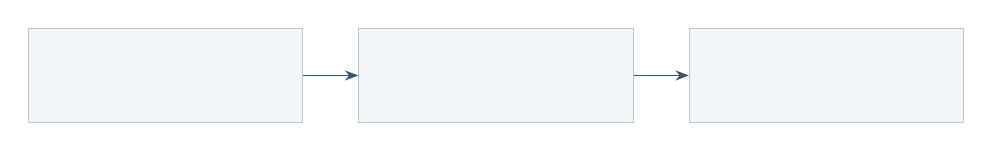
\begin{tikzpicture}[>=Stealth,font=\small]
 \node[draw=ThemeBorder,fill=ThemeBack,text width=3.25cm,align=center,minimum height=1.2cm] (a) {训练集\\拟合参数或保存样本};
 \node[draw=ThemeBorder,fill=ThemeBack,text width=3.25cm,align=center,minimum height=1.2cm,right=7mm of a] (b) {验证集\\选择候选方案};
 \node[draw=ThemeBorder,fill=ThemeBack,text width=3.25cm,align=center,minimum height=1.2cm,right=7mm of b] (c) {测试集\\方案确定后评价};
 \draw[->,ThemeMain] (a)--(b);\draw[->,ThemeMain] (b)--(c);
\end{tikzpicture}
\end{center}
例如比较近邻个数1、3和5，三个候选都只使用训练样本预测，在验证集上比较MAE。选定 $k$ 后再计算测试MAE。如果观察测试结果后继续更换 $k$，测试集已经参与选择，它的分数不再是一次未参与选择的独立最终评价。

最终方案有时会在训练集与验证集合并后重新拟合，再在保留的测试集上评价。这需要在协议中预先规定，尤其要说明合并后重新拟合的具体内容。本章实验为避免混淆，选定 $k$ 后保持原训练集，不做合并重训。

\subsubsection{泛化、欠拟合与过拟合}
\term{泛化}（generalization）指模型对未参与相应拟合或选择的新样本的表现。训练集只是一批有限观测，不能列举未来所有输入。理想目标是降低目标使用环境中的平均错误，而不只是降低训练数据上的平均错误。

\term{欠拟合}（underfitting）表示模型或训练过程未能捕捉数据中与任务有关的规律，常表现为训练与验证都不好。\term{过拟合}（overfitting）表示模型对训练数据中的偶然细节适应过强，新数据表现较差。训练好、验证差是需要检查的信号，但也可能来自错误划分、分布变化或实现不一致，不能只根据两行分数断言原因。

一个极端模型可以记住每个训练编号及其费用。如果预测任务中的新订单有新编号，记忆便无法直接提供有用预测。训练误差为零只说明存储或拟合了已见数据。具有较强表达能力的模型需要足够数据、合理限制和可靠评价，才能判断其优势。

从统计观点，常假设训练和目标新样本来自同一分布，并且样本之间具有适当独立性。该假设有助于把有限样本表现与总体表现联系起来，但现实中可能不满足。费率调整、城市改变、用户行为变化，都可能引起\term{分布变化}（distribution shift）。遇到这种变化，即使先前评价完全合规，模型也可能失效。

\subsubsection{划分方式应模拟实际使用}
随机划分适合样本近似独立、未来使用条件与当前样本混合分布一致的情况。时间划分用较早记录训练、较晚记录评价，更接近预测未来。分组划分让同一用户、设备或病人的记录只进入一个集合，用于评价对新组的泛化。分类中分层划分可尽量保留各集合的类别比例，但它不能替代时间或分组约束。

教学中常见的比例不是普遍规则。数据少时，固定留出集的分数可能波动很大；测试集中少数类过少时，召回率可能缺乏稳定性。第14章将使用交叉验证和不确定性分析处理这些问题。本章重点在于先决定各集合的用途，而不是背诵一个固定百分比。

\begin{infobox}{注意：数据泄漏}
\term{数据泄漏}（data leakage）指拟合或选择过程使用了在规定预测情境中不应获得的信息。包括目标产生后的字段、跨集合的重复或关联记录，以及用全部数据估计预处理规则。泄漏使评价条件偏离实际使用条件，分数可能因此过于乐观。
\end{infobox}
即使标准化没有读取标签，也不应在常规独立测试协议下用测试数据估计均值和方差。它仍然让训练过程利用了测试输入的分布信息。通常先划分，再用训练集拟合预处理规则，最后将同一规则应用到验证和测试。具体算法和特殊协议可能不同，必须明确说明。

\begin{infobox}{例题1.5：一次高分评价的排查}
某模型训练准确率99\%，测试准确率98\%。训练与测试按照片随机划分，其中同一个人的连续拍摄照片出现在两边。应用目标是识别从未出现过的新人的某种表情。这个分数能否直接证明对新人有效？
\end{infobox}
\sol 不能。连续照片共享人物外观、背景和拍摄条件，样本之间有明显关联。照片级随机划分可能让模型在测试时遇到与训练非常接近的输入，而应用要求对新人物有效。

应按人物分组，将某个人的照片全部放在同一集合，重新训练与评价。若需要在新场景使用，还应考虑拍摄场景是否也跨集合。99\%与98\%的接近只能说明当前划分下两组表现接近，无法消除划分与实际目标不一致的问题。

\subsection{评价指标与错误的含义}
\subsubsection{回归指标：MAE、MSE与RMSE}
对评价集中的 $m$ 个样本，真实值为 $y_i$，预测为 $\widehat y_i$，常用
\begin{align}
 \mathrm{MAE}&=\frac1m\sum_{i=1}^{m}|\widehat y_i-y_i|,\\
 \mathrm{MSE}&=\frac1m\sum_{i=1}^{m}(\widehat y_i-y_i)^2,\\
 \mathrm{RMSE}&=\sqrt{\mathrm{MSE}}.
\end{align}
MAE是平均绝对误差，MSE是均方误差，RMSE是均方根误差。这里 $m$ 专指当前评价集合的大小，避免与训练样本数混淆。MAE和RMSE具有与目标相同的单位，MSE具有目标单位的平方。三者都越小越好，但比较时必须使用相同样本、目标单位和计算约定。

如果误差为 $(0,0,0,4)$，MAE为1，RMSE为2。若误差为 $(1,1,1,1)$，两者都为1。MAE在这两个方案间打平，RMSE则更偏好均匀的小误差，因为平方对单个大误差施加更强代价。选择指标因此隐含了对错误分布的偏好。

只看平均值还可能掩盖子群体差异。例如整体MAE较小，但远距离订单误差很大，部署到以远距离订单为主的区域仍会失败。应结合分组结果和具体错例；分组指标样本少时，也要同时报告样本数，不能将偶然变化解释为稳定规律。

\subsubsection{分类指标：先数清四种结果}
二分类中先规定正类，例如“需要检查”。\term{真阳性}（true positive，TP）是实际正类且预测正类；\term{假阳性}（false positive，FP）是实际负类但预测正类；\term{真阴性}（true negative，TN）是实际负类且预测负类；\term{假阴性}（false negative，FN）是实际正类但预测负类。
\begin{center}
\begin{tabular}{lcc}
\toprule
 & 预测正类 & 预测负类\\\midrule
实际正类 & TP & FN\\
实际负类 & FP & TN\\\bottomrule
\end{tabular}
\end{center}
这个表称为\term{混淆矩阵}（confusion matrix）。不同资料可能把实际与预测放在相反轴上，因此读取矩阵时必须先看轴标，不能只凭位置认定哪一格是FP。

\term{准确率}（accuracy）、\term{精确率}（precision）和\term{召回率}（recall）定义为
\begin{align}
 \mathrm{Accuracy}&=\frac{\mathrm{TP}+\mathrm{TN}}{\mathrm{TP}+\mathrm{FP}+\mathrm{TN}+\mathrm{FN}},\\
 \mathrm{Precision}&=\frac{\mathrm{TP}}{\mathrm{TP}+\mathrm{FP}},\\
 \mathrm{Recall}&=\frac{\mathrm{TP}}{\mathrm{TP}+\mathrm{FN}}.
\end{align}
准确率回答“所有判断中有多少正确”；精确率回答“判为正的样本中有多少确实为正”；召回率回答“实际为正的样本中找出了多少”。精确率与召回率的分母不同，不能互换。

若模型从不预测正类，精确率分母为零，数学上未定义；若评价集中没有实际正类，召回率分母为零。程序必须明确处理约定，例如返回缺失标记并报告原因。不能悄悄把未定义值当成真实的0或1，然后与正常指标混合比较。

\begin{infobox}{例题1.6：多数类与准确率陷阱}
100条消息中，实际有5条需要检查。方案A把全部消息判为不需要检查；方案B找出其中4条，但同时错报10条普通消息。比较准确率、精确率与召回率。
\end{infobox}
\sol 方案A的TP为0、FP为0、TN为95、FN为5，因此准确率为95\%，精确率未定义，召回率为0。高准确率来自负类占多数，不能证明模型找到了需要检查的消息。

方案B的TP为4、FP为10、TN为85、FN为1，准确率为 $(4+85)/100=89\%$，精确率为 $4/14\approx28.57\%$，召回率为 $4/5=80\%$。方案B总体准确率较低，却覆盖了大部分正类，同时带来更多人工检查负担。是否有用，需结合漏检与误报成本判断。

\subsubsection{阈值不是模型质量的唯一刻度}
提高正类阈值通常减少被判为正的样本，因此TP与FP都不会增加，召回率通常下降。精确率却不保证单调提高：如果被删除的样本中真阳性的比例高于保留部分，精确率也可能下降。它的实际变化取决于得分排序和标签。

若要求每天最多检查100条消息，就还需要考虑候选数量和排序。若要求漏检率不高于某个水平，应根据验证数据选择阈值，并在未参与选择的数据上核对。阈值的选择属于方案选择，不能在测试集上反复尝试后仍把最好结果当成独立最终评价。

本章只讨论三个基本分类指标。F1、ROC、PR曲线、校准和区间估计会在第14章展开。现阶段的重点是能把指标的每一个分母与具体样本集合对应起来。

\subsection{完整小案例：从数据到最终评价}
\subsubsection{任务、教学数据与比较方案}
假设需要在包裹进入配送系统时，仅根据重量预测费用。简化输入 $x$ 的单位为kg，输出 $y$ 的单位为元。教学数据在约 $0.5$--$6.0$ kg范围内构造，费用大致随重量增加，同时含有小幅偏差。真实费用还受到许多因素影响，本例刻意只保留一个特征，以便手算和逐步追踪。

本例预先固定训练12条、验证4条、测试4条。它不是从真实总体随机抽样得到，因此只能展示协议和计算，不能据此估计真实系统的预期误差。后续项目中必须根据实际采集方式、时间和分组关系建立划分。

\begin{center}
\begin{tabular}{cc@{\qquad}cc@{\qquad}cc}
\toprule
\multicolumn{2}{c}{训练集：前半} & \multicolumn{2}{c}{训练集：后半} & \multicolumn{2}{c}{验证集}\\
$x$/kg & $y$/元 & $x$/kg & $y$/元 & $x$/kg & $y$/元\\\midrule
0.5 & 5.2 & 3.5 & 11.4 & 0.8 & 5.7\\
1.0 & 5.6 & 4.0 & 11.7 & 2.2 & 8.2\\
1.5 & 7.1 & 4.5 & 13.1 & 3.8 & 11.8\\
2.0 & 8.3 & 5.0 & 14.4 & 5.2 & 14.3\\
2.5 & 8.6 & 5.5 & 14.7 & & \\
3.0 & 10.2 & 6.0 & 16.1 & & \\\bottomrule
\end{tabular}
\end{center}
测试输入为 $1.2,2.8,4.2,5.8$ kg，相应标签为 $6.5,9.5,12.3,15.5$ 元。标签虽在讲义中公开，实际执行方案仍须坚持先完成验证选择，再计算测试结果。公开教学数据适于核对代码，不适于模拟长期保密测试集。

比较方案包括均值基线和一个简单的\term{近邻回归}规则。对新重量 $x$，计算它与每个训练重量的距离 $|x-x_i|$，选最近的 $k$ 个训练样本，取这些样本费用的平均值：
\[
 \widehat y(x)=\frac1k\sum_{i\in N_k(x)}y_i.
\]
$N_k(x)$ 是选中训练样本的下标集合，包含 $k$ 项。距离与重量单位相同，费用平均的单位仍为元。候选 $k$ 预先规定为1、3和5；验证MAE越低越好，同分时取较小的 $k$。距离同分时保留训练表中的先后次序，代码中的稳定排序实现这一规则。

\subsubsection{手算一次预测与基线}
验证输入 $x=2.2$ 到训练重量2.0、2.5和1.5的距离分别为0.2、0.3和0.7，其他距离更大。因此
\[
 \widehat y_{k=1}=8.3,\qquad
 \widehat y_{k=3}=\frac{8.3+8.6+7.1}{3}=8.0.
\]
真实值为8.2，所以两种预测的绝对误差分别是0.1和0.2元。该点上 $k=1$ 更好，但选 $k$ 不能只观察这一点，要对整个验证集平均。

训练费用总和为126.4元，训练均值为
\[
 c=\frac{126.4}{12}\approx10.533333\ \text{元}.
\]
均值基线对每个输入都输出这个数。它忽略重量，却利用训练集的总体费用水平。验证集上的四项绝对误差约为4.833333、2.333333、1.266667、3.766667元，平均为3.05元。

\subsubsection{候选选择与最终报告}
将每个候选对四个验证样本的误差平均，得到
\begin{center}
\begin{tabular}{lc}
\toprule
方案 & 验证MAE/元\\\midrule
均值基线 & 3.050000\\
近邻 $k=1$ & 0.100000\\
近邻 $k=3$ & 0.241667\\
近邻 $k=5$ & 0.540000\\\bottomrule
\end{tabular}
\end{center}
依照预定规则选 $k=1$。保持原训练集，在测试集上预测，得到
\begin{center}
\begin{tabular}{ccccc}
\toprule
$x$/kg & 真实费用/元 & 预测费用/元 & 预测减真实/元 & 绝对误差/元\\\midrule
1.2 & 6.5 & 5.6 & $-0.9$ & 0.9\\
2.8 & 9.5 & 10.2 & 0.7 & 0.7\\
4.2 & 12.3 & 11.7 & $-0.6$ & 0.6\\
5.8 & 15.5 & 16.1 & 0.6 & 0.6\\\bottomrule
\end{tabular}
\end{center}
最终测试MAE为 $(0.9+0.7+0.6+0.6)/4=0.7$ 元，均值基线测试MAE为2.95元。验证与测试MAE不同是正常现象，它们包含不同样本。测试只有4条，更不能将0.7元当作某个真实总体的精确平均误差。

这个结果支持的结论是：在当前固定教学划分上，按验证集选出的近邻规则优于指定均值基线。它不支持“近邻必然优于线性回归”，因为没有进行相应比较；也不支持“实际配送误差不超过0.7元”，因为平均误差不限制每个样本，更没有实际数据证据。

\subsubsection{适用边界与可复现步骤}
当输入 $x=10$ kg时，$k=1$ 仍取最接近的6.0 kg训练样本，输出16.1元。它不会根据重量继续增长自动推算费用。输入落在已见范围之外的预测称为\term{外推}（extrapolation）；这种边界行为提醒模型有自己的归纳规则，不能只因范围内结果好就信任范围外结果。

本例的执行顺序为：固定任务与数据划分，拟合基线或保存训练记录，计算验证指标，选定候选，计算一次最终测试指标，检查逐样本误差并说明局限。其完整预测计算通过对 $n$ 个训练距离排序完成，每个查询通常需要 $O(n\log n)$ 排序时间，保存训练表需要 $O(n)$ 空间。这里的记号只表示增长趋势：数据规模翻倍，排序成本会增长；不是精确运行秒数。第15章将讨论更高效的实现。

\begin{infobox}[unbreakable]{注意：简化实现的边界}
本例只有一个数值特征、20条构造记录，无缺失值和复杂编码。它展示完整学习流程的骨架。实际项目仍需要数据质量检查、合适划分、预处理、更多基线、统计不确定性和部署后的监测。
\end{infobox}

\subsection{实验1.1：可运行的近邻预测流程}
\subsubsection{环境、输入与运行}
代码入口为\code{ch01_regression.py}，保存在“配套实验”目录。使用Python 3标准库，不读取外部文件，不下载数据，不安装第三方库。在该目录打开终端后运行：
\begin{console}
python3 ch01_regression.py
\end{console}
Windows环境若Python由启动器管理，可用\code{py -3 ch01_regression.py}。解释器和终端的区别在第2章说明。此时可以先看输出、手算核对，再于第二章后阅读函数细节。

数据列表与上一节完全对应。核心函数如下：
\begin{pycode}
def neighbor_predict(data, x, k):
    if not 1 <= k <= len(data):
        raise ValueError("invalid k")
    ordered = sorted(data, key=lambda row: abs(row[0] - x))
    selected = ordered[:k]
    return sum(y for _, y in selected) / k


def mae(data, predict):
    errors = [abs(predict(x) - y) for x, y in data]
    return sum(errors) / len(errors)
\end{pycode}
\code{data}包含若干 $(x_i,y_i)$ 对。第2行检查 $k$ 是否在1到训练数量之间；第4行按距离排序，\code{row[0]}取训练重量；第5行只保留前 $k$ 条；第6行把费用相加后除以 $k$。\code{lambda}是一个短的匿名函数，这里只表达“按重量距离排序”，无需在本章掌握语法。

\code{mae}接受一个预测函数，对评价样本逐个计算绝对误差，最后平均。这样指标函数不必知道预测来自均值、近邻还是其他模型。代码中的函数式组织会在第二章函数一节再次分析。

\subsubsection{选择逻辑与预期输出}
\begin{pycode}
results = []
for k in [1, 3, 5]:
    score = mae(valid, lambda x: neighbor_predict(train, x, k))
    results.append((score, k))
_, best_k = min(results)
final_score = mae(
    test, lambda x: neighbor_predict(train, x, best_k)
)
\end{pycode}
每个候选使用同一份\code{train}。验证标签只进入误差计算，未被传给近邻预测函数。\code{results}保存“验证分数、邻居数”对；\code{min}按元组先比较分数，再比较 $k$，实现预定同分规则。最终测试行位于选择之后。

完整脚本预期主要输出为：
\begin{console}
split sizes: 12 4 4
baseline validation MAE: 3.050000
k=1 validation MAE: 0.100000
k=3 validation MAE: 0.241667
k=5 validation MAE: 0.540000
selected k: 1
baseline test MAE: 2.950000
selected model test MAE: 0.700000
\end{console}
随后还会打印四个测试样本的预测和误差。输出保留六位小数是显示约定，不表示原始费用测量有六位小数精度。使用相同数据和规定排序规则时，应得到相同的打印结果；浮点内部结果与手算小数允许约 $10^{-9}$ 的绝对差异。

\subsubsection{修改任务与结果解释}
先将训练标签的第二项5.6改成9.6，重新运行，并手算验证输入0.8和测试输入1.2的最近邻预测。修改的是训练数据，允许重新执行完整选择；应记录这一变化，不能把新输出与原实验视为同一次固定评价。

再增加一个待预测重量10.0，只打印预测，不把它混入原测试MAE。该输入没有真实标签，不能计算正确误差。观察输出是否随重量继续线性增长，并联系上一节的外推限制。

最后尝试令 $k=0$ 或 $k=13$，确认程序主动拒绝不合法邻居数。如果删去检查，$k=0$ 会导致除以零；$k=13$ 则只有12个样本被选中，却错误地除以13。这说明边界检查不仅为防止程序崩溃，也为防止产生看似正常但数学意义错误的数值。

\subsection{实验1.2：阈值、混淆矩阵与检查成本}
\subsubsection{输入与目标}
代码入口为\code{ch01_classification.py}。八条消息的标签与固定分数为
\begin{center}
\begin{tabular}{c*{8}{c}}
\toprule
下标 & 0 & 1 & 2 & 3 & 4 & 5 & 6 & 7\\\midrule
标签 & 1 & 1 & 0 & 0 & 1 & 0 & 0 & 0\\
分数 & .90 & .60 & .80 & .30 & .40 & .20 & .55 & .10\\\bottomrule
\end{tabular}
\end{center}
标签1表示需要检查，0表示不需要。分数在本实验中是人为给定的示意值，不宣称具有已校准概率含义。实验不训练分类模型，只分析从固定分数到类别的过程。因此本表也不是用于选定真实业务阈值的最终测试集。

先以阈值0.5手算预测：下标0、1、2、6判为正，其余判为负。逐条对照标签得到TP=2、FP=2、TN=3、FN=1。阈值0.7时只有下标0、2判为正，得到TP=1、FP=1、TN=4、FN=2。

\subsubsection{实现与逐条核对}
\begin{pycode}
tp = fp = tn = fn = 0
for label, score in zip(labels, scores):
    predicted = int(score >= threshold)
    if label == 1 and predicted == 1:
        tp += 1
    elif label == 0 and predicted == 1:
        fp += 1
    elif label == 0 and predicted == 0:
        tn += 1
    else:
        fn += 1
\end{pycode}
\code{zip}将相同位置的标签和分数配成一对。\code{score >= threshold}得到真假值，转成整数后真为1、假为0。四个分支互斥，每条有效二分类记录恰好使一个计数加1。完整脚本在循环前检查长度一致且非空，本实验输入预先保证标签属于0或1。

运行
\begin{console}
python3 ch01_classification.py
\end{console}
得到
\begin{console}
threshold: 0.5
TP FP TN FN: 2 2 3 1
accuracy=0.625000 precision=0.500000 recall=0.666667
threshold: 0.7
TP FP TN FN: 1 1 4 2
accuracy=0.625000 precision=0.500000 recall=0.333333
\end{console}
两个阈值准确率都为 $5/8$，精确率都为 $1/2$，召回率却从 $2/3$ 降至 $1/3$。因此只观察准确率，可能看不出漏检增加。所有计数应与手算完全一致；分数仅存在打印舍入差异。

\subsubsection{修改任务}
假设一次误报成本为1，一次漏检成本为5，定义总错误成本为 $C=\mathrm{FP}+5\mathrm{FN}$。阈值0.5的成本为7，阈值0.7的成本为11。成本单位是人为定义的统一代价，不能在没有实际业务估计时当成真实金额。

将下标4的分数由0.4改成0.6，其标签仍为1。先不运行程序，分别预测两个阈值下四个计数怎样变化，再运行核对。还可将阈值设为1.1，检查“没有预测正类”的情形：精确率返回\code{None}，召回率为0。完整脚本的固定格式打印为两个正常阈值设计；扩展到未定义精确率时，应先判断\code{None}再决定显示字符串，不能直接套用小数格式。

\subsection{知识联系、常见误区与自检}
从问题到结果可用一条因果关系清楚的工作链描述：任务决定可用信息与目标；目标和错误成本决定评价；数据采集与划分决定评价条件；模型和训练算法决定候选预测规则；验证决定选择；测试提供在该协议下的结果。这条链中任何一环出现偏差，都可能使精确计算得到的分数失去原本含义。

本章常见误区有以下几类。把AI与神经网络等同，会忽略搜索和规则等方法；把所有数字目标当成回归，会给类别编号施加虚假的大小关系；把训练损失低当成新数据可靠，会忽略泛化；把验证和测试互换，会让最终结果受到选择影响；把评分当成概率，会误解阈值；把平均误差当成最大误差，会低估异常样本风险。

模型表现还不是因果结论。若较重的包裹往往同时使用更远的路线，模型可能利用重量预测费用，但这不证明“仅增加重量就会使费用按同样规律变化”。预测描述已观测关系，因果问题需要额外假设、设计或证据。本书主线首先建立预测建模与可靠评价基础。

完成本章后，应能不看公式解释MAE分母是什么；用具体记录说明FP与FN；给出一个预测时不可用的字段；解释为何选 $k$ 要读验证集而非测试集；说明一个实验结论的适用范围。如果只能复述名词而无法对新场景作上述判断，应回到任务卡和两个实验逐项对应。

\subsection{分层习题}
以下题目编号为1.1--1.12。概念题要求用完整任务说明回答，计算题需写出中间量，实验题需同时给出数值与结论的边界。
\begin{enumerate}[label=\textbf{1.\arabic*}]
\item \textbf{概念。}固定规则判断银行卡号格式、从标注图片学习识别缺陷、对文本预测下一个词元、在网格中根据奖励学习移动，分别对应什么方法或学习方式？能否把固定规则排除出所有人工智能系统？
\item \textbf{任务定义。}“预测学生成绩”过于含糊。以学期开始时预测期末分数为目标，写出样本单位、预测时点、三个候选输入、一个不能使用的字段和一个评价指标。说明标签单位。
\item \textbf{数据表示。}200张图像已被表示为每张64个数值，标签有5类。写出 $X$ 的形状；类别标签必须表示为 $200\times5$ 矩阵吗？若采用整数类别编号，怎样解释编号？
\item \textbf{计算。}真实值为 $(2,4,6)$，预测为 $(3,4,4)$。计算残差、MAE、MSE与RMSE，并说明目标单位为元时各指标的单位。
\item \textbf{训练目标。}标签为 $(2,2,8)$。求平方损失下最佳常数预测与相应MSE；再比较常数2与常数4的MAE。解释为什么均值基线不一定是MAE最优基线。
\item \textbf{模型选择。}候选A、B、C的训练MAE分别为0.2、0.5、0.8，验证MAE分别为1.5、0.7、0.9。按最小验证MAE规则选哪个？能否从这些分数确定A一定发生了过拟合？
\item \textbf{泄漏判断。}预测订单最终费用时，分别讨论使用最终付款状态、在全部数据上拟合填补均值、同一订单复制记录跨入训练和测试。写出每种情况的修正措施。
\item \textbf{分类计算。}20个实际正类、80个实际负类中，模型找到15个正类，同时错报12个负类。给出混淆矩阵、准确率、精确率与召回率。将正类改成“普通消息”后，原FP对应新的哪种错误？
\item \textbf{划分。}同一用户有多条记录，数据跨越两年。任务甲是预测已有用户的下一次购买；任务乙是预测全新用户是否购买。分别提出合适的主要划分约束，说明为什么随机按行划分不一定合理。
\item \textbf{手算近邻。}训练记录为 $(1,5),(2,7),(4,11),(5,13)$。对 $x=3.2$ 计算 $k=1$ 和 $k=3$ 的预测；若真实值为10，比较绝对误差。对 $x=8$ 的 $k=1$ 预测又是多少？
\item \textbf{实验。}在实验1.2中把下标4的分数改成0.6，其他不变。分别计算阈值0.5和0.7的指标、成本 $\mathrm{FP}+5\mathrm{FN}$，并运行程序核对。若要选择真实系统阈值，还需要哪些数据安排？
\item \textbf{综合。}某报告写道：“尝试100次后选出测试准确率最高的模型，准确率97\%，因此任何未来消息都至少有97\%概率被正确处理。”指出报告中的两个不同错误，并改写为条件明确的报告流程。
\end{enumerate}

\subsection{习题参考答案}
\subsubsection*{1.1--1.3：概念与数据}
\textbf{1.1}\quad 银行卡号格式判断使用人工给定的规则，不必从样本学习；缺陷识别是监督分类；下一词元预测是从文本构造目标的自监督学习；按交互奖励学习移动是强化学习。固定规则可以成为AI系统的一部分，例如约束输出、组织推理或校验数据，但不能仅因使用计算机和条件语句，就把任意普通程序都赋予一个有实质意义的AI能力结论。

\textbf{1.2}\quad 样本单位为某个学期的一名学生，预测时点为学期开始前或开始时，需明确到数据可用截止时刻。候选输入可以是先修课程成绩、已完成课程数量、当前课程类别；期末考试得分本身、期末后的教师评分与全学期出勤汇总均不能作为此时输入。标签为该学期最终分数，假设满分100，单位为分。可用MAE评价，另检查不同课程或历史水平群体的误差。该示例是任务定义练习，不假设这些输入足以产生可靠预测。

\textbf{1.3}\quad $X\in\mathbb R^{200\times64}$。标签可以是长度200的整数序列，每项属于 $\{0,1,2,3,4\}$；也可以根据算法需要使用其他编码，并非必须为 $200\times5$。整数是类别代号，不意味着类别4是类别2的两倍，也不宜对代号直接计算回归误差。

\subsubsection*{1.4--1.6：损失与选择}
\textbf{1.4}\quad 以预测减真实定义残差，得到 $(1,0,-2)$。绝对值为 $(1,0,2)$，平方为 $(1,0,4)$，所以
\[
 \mathrm{MAE}=1,
 \qquad\mathrm{MSE}=\frac53,
 \qquad\mathrm{RMSE}=\sqrt{\frac53}\approx1.2910.
\]
MAE与RMSE单位为元，MSE单位为元$^2$。残差平均为 $-1/3$，它不能代替MAE，因为正负错误可能抵消。

\textbf{1.5}\quad 训练均值为 $(2+2+8)/3=4$。平方误差为 $(4,4,16)$，MSE为8。常数2的MAE为 $(0+0+6)/3=2$，常数4的MAE为 $(2+2+4)/3=8/3$。均值优化平方损失，中位数2在本例中给出更小的绝对损失。两种目标对偏离较大的8赋予不同权重。

\textbf{1.6}\quad 选B，因为验证MAE为0.7，三者中最低。A训练很低但验证高，符合需要排查过拟合的现象，也可能受划分偏差、分布变化或预测实现错误影响。应检查流程后再诊断，不能仅靠两个指标证明唯一原因。C训练与验证都较高，可能模型能力不足或训练不充分，也要结合具体目标判断。

\subsubsection*{1.7--1.9：评价条件}
\textbf{1.7}\quad 最终付款状态产生在预测时点之后，应屏蔽该字段或重新定义预测时点。全数据填补均值把测试输入信息用于处理规则，应先划分，仅从训练集估计均值，再应用到其他集合。复制的订单跨集合会使测试包含训练已见实例，应先识别重复并按订单标识整体分配。去重规则需保留真正不同的订单，不能只因重量相同便删除。

\textbf{1.8}\quad TP=15、FN=5、FP=12、TN=68。准确率为 $83/100=83\%$，精确率为 $15/27\approx55.56\%$，召回率为 $15/20=75\%$。若正负类整体交换，原来“实际负、预测正”的FP变成“实际正、预测负”的FN。这说明错误名称依赖正类约定。

\textbf{1.9}\quad 任务甲应以时间为主要约束，训练用较早记录，评价用后续记录；同一用户可按任务需要在前后时期出现，但只能使用截止时刻以前的信息。任务乙应以用户分组为主要约束，测试用户不能在训练中出现；若部署还面向后续时间，应同时设计时间边界。随机按行会混合前后时期，也会让同一用户跨集合，可能偏离两个任务中要求的条件。

\subsubsection*{1.10--1.12：计算、实验与报告}
\textbf{1.10}\quad 对3.2，四个距离依次为2.2、1.2、0.8、1.8。最近一个是 $(4,11)$，所以 $k=1$ 预测11，误差1。最近三个依次为 $(4,11),(2,7),(5,13)$，预测 $31/3\approx10.3333$，误差 $1/3$。该点上 $k=3$ 更好，不能从一个点决定全局最优。对8，最近为 $(5,13)$，$k=1$ 预测13，表现为边界常值而非继续增长。

\textbf{1.11}\quad 阈值0.5时，下标4由漏检变为检出，TP=3、FP=2、TN=3、FN=0。准确率 $6/8=0.75$，精确率 $3/5=0.6$，召回率1，成本2。阈值0.7时该样本仍被判负，因此计数与原实验相同，准确率0.625，精确率0.5，召回率 $1/3$，成本11。真实系统需要独立训练与验证数据，在验证集选阈值，保留测试集作最终评价，并确保类别比例、采集条件和成本定义与实际使用相符。

\textbf{1.12}\quad 第一个错误是反复使用测试集选模型，它已经成为选择数据；第二个错误是把有限集合上的平均正确比例解释为每个未来消息都满足的概率下界。未来分布可能变化，个体错误概率也不相同。

可先固定任务、划分和指标，用训练集拟合，用验证集完成100次候选比较，记录选择规则；选定方案后只作一次保留测试评价，并报告测试样本数、类别比例、指标和采集条件。若测试数据已被用于比较，需要另行准备未参与选择的评价数据。报告只陈述指定协议下观察到的结果，再分析不确定性与适用边界。

\subsection{本章小结}
机器学习通过数据或交互经验改进任务表现，深度学习和大语言模型是其中的重要方法与模型类别。学习方式取决于训练信号来源，任务类型取决于希望获得的输出。样本、特征、标签定义了数据，模型、参数、训练目标和算法定义了拟合过程，验证与测试定义了选择和最终评价的职责。

实际任务必须交代预测时点、可用字段、目标单位、评价对象和错误代价。训练表现、有限测试表现与未来总体表现是不同对象。下一章建立运行和阅读实验所需的Python基础，将本章的逐样本计算变成可核对的程序。

\chapterpage{Python语言基础}\label{ch:python}
\begin{infobox}{先修知识、学习目标与本章位置}
本章从运行程序开始，只要求基本算术和第一章中的样本、误差概念。学习后应能区分终端、解释器与编辑器；运行并修改脚本；使用基本类型、条件、循环和容器；编写具有明确输入、输出和边界条件的函数；按顺序追踪程序中的数值变化。

本章使用Python 3，不使用NumPy或机器学习库。配套实验只依赖标准库。模块、文件读写、异常的完整机制、对象引用与调试流程在第3章继续；本章提前使用的少量输入检查会给出局部解释，不以此替代后续系统讨论。
\end{infobox}
机器学习实验把输入表示为程序对象，将公式中的逐项运算写为表达式，再利用循环或库函数处理许多样本。程序出现错误时，需要能够判断问题出在数据、控制流程还是计算规则。本章先建立这种基本阅读与编写能力，随后才进入数组和向量化。

程序的核心不是记住所有语法，而是对每一步的状态作出明确判断：这一行读取哪些值、产生什么值、修改了什么对象、下一行从哪里继续。为此，本章使用小规模且可手算的数据，并在重要代码后提供逐行分析。

\subsection{运行程序：解释器、终端与编辑器}
\subsubsection{三个工具的职责}
\term{解释器}（interpreter）执行Python程序。\term{终端}（terminal）提供输入系统命令的窗口，窗口内通常由命令行\term{Shell}解析命令。\term{编辑器}（editor）用于创建、保存和修改文本文件。集成开发环境可以把编辑、终端和运行按钮放在同一个窗口，但这些职责仍然不同。

终端里输入\code{python3 hello.py}，Shell启动Python解释器，再让解释器执行\code{hello.py}中的代码。Python交互环境里输入\code{2 + 3}，则是已经启动的解释器直接计算表达式。若把\code{python3 hello.py}写进Python文件，它不是一条合法Python语句；若在普通终端直接输入\code{print(2 + 3)}，也不等于让Python运行这段代码。

\begin{center}
\begin{tabularx}{\linewidth}{l Y Y}
\toprule
位置 & 输入内容示例 & 实际负责者\\\midrule
普通终端 & \code{python3 hello.py} & Shell启动解释器\\
Python交互环境 & \code{2 + 3} & 解释器求值\\
文本编辑器 & \code{print(2 + 3)} & 保存代码，运行时才执行\\
程序输出区域 & 数字\code{5} & 显示结果，不是新代码\\\bottomrule
\end{tabularx}
\end{center}
本章代码框中的行号仅用于说明，不属于程序文本。终端命令框不含行号。将代码复制到文件时，不要加入解释器的提示符\code{>>>}，也不要复制输出结果。

\subsubsection{检查解释器与第一次交互}
在macOS或Linux终端中运行
\begin{console}
python3 --version
\end{console}
它应打印Python 3的版本信息。Windows可尝试\code{py -3 --version}；若系统将命令注册为\code{python}，也可使用\code{python --version}，但需确认确实是Python 3。若命令不存在，说明解释器未安装、启动器未配置或路径未设置，应通过Python官方安装说明处理，不能把未找到命令误认作程序语法错误。

随后运行\code{python3}，进入交互环境。下列框为输入与输出的完整示意：
\begin{console}
>>> 2 + 3
5
>>> value = 8
>>> value * 2
16
>>> print(value)
8
>>> exit()
\end{console}
\code{>>>}是解释器显示的提示符。赋值行\code{value = 8}通常不自动打印值，表达式\code{value * 2}在交互环境会显示求值结果。\code{exit()}离开交互环境，返回普通终端。此后才输入执行脚本的系统命令。

\subsubsection{保存与运行脚本}
\term{脚本}（script）是包含程序文本的文件。创建UTF-8编码的纯文本文件\code{hello.py}，保存如下内容：
\begin{pycode}
name = "Python"
count = 3
print("language:", name)
print("count:", count)
print(2 + count)
\end{pycode}
在文件所在目录打开终端，运行\code{python3 hello.py}，输出应为
\begin{console}
language: Python
count: 3
5
\end{console}
解释器按顺序执行：先把名称\code{name}绑定到字符串，把\code{count}绑定到整数，再进行三次打印。\code{print}括号中的多个项默认用空格分隔，打印后换行。

脚本中的单独表达式\code{2 + count}会被计算，但通常不显示结果。若要看到它，必须写\code{print(2 + count)}。这是交互环境和脚本在初学阶段最容易混淆的区别之一。

\subsubsection{目录、路径与空格}
终端有\term{当前工作目录}。相对文件名\code{hello.py}会在当前目录中寻找，不会自动在整个电脑上搜索。macOS或Linux使用\code{pwd}查看当前目录，\code{ls}查看文件；Windows命令提示符可用\code{cd}显示当前目录、\code{dir}列出文件。

本讲义配套实验位于含中文和空格的目录，可在macOS终端中运行：
\begin{console}
cd "/Users/mac/Desktop/机器学习 ML/配套实验"
python3 ch02_basics.py
\end{console}
路径两侧的引号让Shell把它看成一个整体。这里的引号用于系统命令中的路径，不是Python文件中的字符串定义。也可以使用脚本的绝对路径运行，不必先切换目录；但更复杂的程序可能读取相对文件，届时工作目录仍需核对。

保存时应核对扩展名。正确名称为\code{hello.py}；若名称为\code{hello.py.txt}，实际仍是文本扩展名。代码中的括号、冒号、引号和逗号使用英文半角符号。中文全角冒号或智能引号看起来相近，却不属于相同的语法字符。

\subsection{虚拟环境、标准库与依赖}
\subsubsection{为什么区分环境}
\term{标准库}随Python提供，包含数学、随机数、文件路径等许多功能。\term{第三方包}是另外安装的代码，例如后续使用的NumPy、pandas和PyTorch。程序所依赖的包及其版本称为\term{依赖}（dependency）。本章四个实验无需安装第三方包。

不同项目可能要求不同包版本。如果把所有包混装在一个环境中，一次升级可能影响另一项目。\term{虚拟环境}（virtual environment）为一个项目隔离包安装位置，并提供与该环境关联的解释器入口。它不是虚拟机，不会另建一套完整操作系统。

在项目目录中创建环境：
\begin{console}
python3 -m venv .venv
\end{console}
\code{-m venv}表示让选定的解释器运行标准库中的\code{venv}模块；\code{.venv}是环境目录名。创建成功后，再根据Shell激活：
\begin{center}
\begin{tabularx}{\linewidth}{l Y}
\toprule
终端类型 & 激活命令\\\midrule
macOS/Linux的常见Shell & \code{source .venv/bin/activate}\\
Windows命令提示符 & \texttt{.venv\textbackslash{}Scripts\textbackslash{}activate.bat}\\
Windows PowerShell & \texttt{.venv\textbackslash{}Scripts\textbackslash{}Activate.ps1}\\\bottomrule
\end{tabularx}
\end{center}
激活后通常使用\code{python}调用环境解释器，退出可用\code{deactivate}。PowerShell可能受脚本执行策略限制；可按官方说明处理，或直接调用环境解释器，无须为运行本章实验修改系统级策略。

\subsubsection{安装位置与解释器对应}
无需激活也可以明确调用环境中的解释器，macOS/Linux为\code{.venv/bin/python}，Windows为\texttt{.venv\textbackslash{}Scripts\textbackslash{}python.exe}。这种方式减少“包安装到了一个环境，脚本却在另一个环境运行”的混淆。

需要安装第三方包时，优先使用\code{python -m pip}，例如后续章节的环境中可能运行\code{python -m pip install numpy}。这会使用当前指定解释器对应的包管理工具。安装不是本章的实验步骤，提前安装机器学习库也不能代替掌握基础语法。

编辑器可能另有解释器选择设置。即使终端激活了环境，编辑器运行按钮也不必自动采用相同解释器。可用下列小程序查看实际执行者：
\begin{pycode}
import sys
print(sys.executable)
print(sys.version)
\end{pycode}
\code{import sys}导入标准库模块，下一行打印解释器路径，再下一行打印版本。模块的一般组织方式将在第3章展开。此处只把这段程序作为环境核对工具。

\begin{infobox}{注意：环境准备的最小要求}
能确认Python 3解释器、保存UTF-8脚本并在正确目录运行，就能完成本章实验。虚拟环境为后续依赖管理建立习惯；它不会改变\code{if}、\code{for}、列表或函数的基本语义。
\end{infobox}

\subsection{变量、赋值、对象与表达式}
\subsubsection{名称绑定与顺序执行}
\term{变量}在本章可理解为指向某个值的名称。更准确地说，赋值建立名称与对象的绑定。写\code{weight = 2.5}时，右边表达式先求值，再把左边名称绑定到结果。\code{=}不是数学中两个表达式永远相等的声明。
\begin{pycode}
x = 3
x = x + 2
y = 2 * x
print(x, y)
\end{pycode}
第一行后\code{x}为3；第二行先读取旧\code{x}，算出5，再更新绑定；第三行读取当前\code{x}，得到\code{y}为10。最终输出\code{5 10}。不存在代数方程 $x=x+2$ 所导致的矛盾，因为它描述了两个不同执行时刻。

如果名称还未赋值就被读取，例如脚本第一行直接写\code{print(weight)}，会产生\code{NameError}。给名称赋值时不需要先声明固定类型，但对象具有类型。\code{count = 3}后又写\code{count = "three"}是允许的；后续代码若期待数字，仍可能产生类型错误。因此名称应保持稳定含义，避免随意切换角色。

\subsubsection{命名与注释}
名称可以包含字母、数字和下划线，不能以数字开头，不能使用\code{for}、\code{if}等关键字。Python允许部分Unicode名称，本讲义代码采用清晰的英文名称与下划线，例如\code{train_size}、\code{predicted_cost}。大小写不同表示不同名称：\code{Score}和\code{score}不相同。

不要将\code{sum}、\code{list}、\code{str}、\code{min}等常用内置功能名称用作变量。若写\code{sum = 10}，再写\code{sum(values)}，名称已经指向整数，便不能作为函数调用。变量名称应表达意义，而不是仅方便输入。

\texttt{\#}后直到行末为\term{注释}，解释器不执行这些文字。注释应解释规则、单位或约束，而不是重复显而易见的代码。如下写法记录了单价单位：
\begin{pycode}
price_per_kg = 2.0  # unit: yuan per kg
weight_kg = 3.5
cost_yuan = price_per_kg * weight_kg
\end{pycode}
字符串中的\texttt{\#}只是普通字符，例如\texttt{"order\#17"}。长说明可以放在文档字符串中，函数一节会给出示例。

\subsubsection{表达式、语句与增强赋值}
\term{表达式}求出一个值，例如\code{2 * x + 1}、\code{score >= 60}或\code{len(values)}。\term{语句}执行某种动作或控制流程，例如赋值、条件分支和循环。函数调用既可以在表达式中提供返回值，也可以作为独立语句执行。

\code{total += value}在数值累加场景中相当于把\code{total + value}的结果重新赋给\code{total}。它不能省略初始化：第一次累加前要给\code{total}赋初值。容器的增强赋值可能涉及对象修改，引用与副作用的完整区别将在第3章讨论，本章主要使用数值累加。

多重赋值如\code{a, b = 2, 5}先求右边，再绑定左右对应名称；\code{a, b = b, a}因此能交换数值。若分两行\code{a = b}、\code{b = a}，第一行已经覆盖旧\code{a}，第二行将得到与\code{a}相同的值。

\begin{infobox}{例题2.1：赋值追踪与交换}
执行下列代码后，\code{a}、\code{b}和\code{c}分别是多少？为什么？
\end{infobox}
\begin{pycode}
a = 4
b = a + 3
a = 2 * a
c = b - a
a, b = b, a
print(a, b, c)
\end{pycode}
\sol 第1行建立\code{a=4}。第2行得到\code{b=7}。第3行把\code{a}改为8，不会让先前计算好的\code{b}重新计算。第4行得到\code{c=-1}。第5行同时使用旧\code{b=7}和旧\code{a=8}，交换后\code{a=7,b=8}。输出为\code{7 8 -1}。变量不是自动维护的电子表格公式，修改输入名称不会回溯执行旧语句。

\subsection{数值类型、运算与浮点误差}
\subsubsection{整数、浮点数与类型转换}
\term{整数}类型为\code{int}，例如3、0和$-7$；\term{浮点数}类型为\code{float}，例如3.0、0.25和\code{1e-3}。科学计数形式\code{1e-3}表示 $10^{-3}$。Python整数可以随数值增长使用更多存储空间，不等于机器学习数组中的固定宽度整数；浮点数精度则有限。

用\code{type(value)}查看类型。\code{int(3.9)}得到3，它朝零截断，并不是四舍五入；\code{int(-3.9)}得到$-3$。\code{float("3.5")}把合法数字字符串转为浮点数，\code{int("3.5")}会失败，因为该字符串不是整数格式。\code{str(3.5)}则产生文本\code{"3.5"}，不再是可直接进行数值加法的浮点数。

类型转换需要有数据规则。用户输入\code{"abc"}不能直接转为浮点数；空串也不能。字符串中有数字并不保证整体是合法数字，例如\code{"score=82"}。完整输入校验与异常处理在第3章学习，本章实验采用范围有限且能事先辨认的整数文本。

\subsubsection{运算符与优先级}
\begin{center}
\begin{tabularx}{\linewidth}{c Y Y}
\toprule
符号 & 含义 & 示例与结果\\\midrule
\code{+ - *} & 加、减、乘 & \code{3 * 4}为12\\
\code{/} & 真除法 & \code{7 / 2}为3.5\\
\code{//} & 向下取整除法 & \code{7 // 2}为3\\
\texttt{\%} & 余数 & \texttt{7 \% 2}为1\\
\code{**} & 幂 & \code{2 ** 3}为8\\
\code{abs(x)} & 绝对值 & \code{abs(-2)}为2\\\bottomrule
\end{tabularx}
\end{center}
加减低于乘除，幂的优先级较高；应优先通过括号明确数学意义。均方误差的一项应写\code{(prediction - target) ** 2}，若写\code{prediction - target ** 2}，只会把真实值平方再相减。

负数除法尤其需要核对：\code{-7 // 2}为$-4$，因为 $-3.5$ 向下取整到$-4$，不是朝零截断到$-3$。配套余数\texttt{-7 \% 2}为1，仍满足
\[
 a=(a//b)\,b+(a\%b),\qquad b\ne0.
\]
若 $a,b$ 都为整数，则这些算术规则可用于整除与余数判断。写\texttt{i \% 2 == 0}判断整数是否偶数。除数为零会报错，不能将“没有样本”的平均值直接计算为\code{total / 0}。

\code{-2 ** 2}得到$-4$，解析为\code{-(2 ** 2)}；\code{(-2) ** 2}得到4。多层幂如\code{2 ** 3 ** 2}按\code{2 ** (3 ** 2)}解释。复杂表达式宜用括号和中间名称分解，减少依赖记忆优先级。

\begin{infobox}{例题2.2：把数学式译为程序}
给定预测 $\widehat y=9$、真实值 $y=6$，计算绝对误差、平方误差，以及 $\sqrt{\frac{1+4+9}{3}}$。写出不会混淆优先级的代码。
\end{infobox}
\begin{pycode}
prediction = 9
actual = 6
absolute_error = abs(prediction - actual)
squared_error = (prediction - actual) ** 2
root_mean_square = ((1 + 4 + 9) / 3) ** 0.5
print(absolute_error, squared_error, root_mean_square)
\end{pycode}
\sol 绝对误差为3，平方误差为9，最后一项为 $\sqrt{14/3}\approx2.160246899$。第5行先求和、再平均、最后开方，括号直接对应公式结构。指数0.5在非负实数上用于平方根；这里被开方量非负，条件满足。

\subsubsection{浮点数不是所有小数的精确表示}
常见Python浮点数使用有限位二进制表示。十进制有限小数不一定有有限二进制展开，类似 $1/3$ 在十进制中必须近似。因此
\begin{pycode}
print(0.1 + 0.2)
print(0.1 + 0.2 == 0.3)
\end{pycode}
通常输出\code{0.30000000000000004}和\code{False}。这不是加法规则改变，而是输入数值和运算结果以邻近的可表示数近似。

\code{round(value, 2)}和格式化保留两位小数可以改善显示，但不能让任意内部数值变成精确十进制数。\code{round}还采用特定的舍入规则，对恰好中点的可精确表示数倾向于保留偶数，例如\code{round(2.5)}为2、\code{round(3.5)}为4。\code{round(2.675, 2)}可能为2.67，因为2.675本身已被二进制近似，不宜仅用十进制手工舍入直觉推断。

对计算结果检查，应采用容差：
\begin{pycode}
import math
value = 0.1 + 0.2
print(math.isclose(value, 0.3, rel_tol=1e-9, abs_tol=1e-12))
\end{pycode}
输出\code{True}。\code{rel_tol}随数值规模设定相对容差，\code{abs_tol}为接近零的比较提供绝对容差。大致判断条件为
\[
 |a-b|\le\max\bigl(r\max(|a|,|b|),\varepsilon\bigr),
\]
其中 $r$ 为相对容差，$\varepsilon$ 为绝对容差。具体容差应依目标单位、计算误差和问题要求设定，而不是所有问题都固定使用同一值。

\begin{infobox}[unbreakable]{注意：误差来源需要区分}
输入测量误差、有限样本造成的统计波动、模型预测误差和计算机浮点舍入误差，是不同来源。显示更多小数不能减少前几种误差。对费用、成绩等问题，首先保持单位与计算规则一致，再讨论数值精度。
\end{infobox}

\subsection{字符串、输入与输出}
\subsubsection{字符串及其索引}
\term{字符串}（string，\code{str}）表示文本，使用单引号或双引号包围，例如\code{"train"}。引号不是字符串内容的一部分。\code{"12" + "3"}得到\code{"123"}，\code{12 + 3}得到15；\code{"12" + 3}因类型不兼容而失败。

字符串可拼接或重复：\code{"ab" * 3}得到\code{"ababab"}。\code{len(text)}给出字符串长度；\code{text[0]}读取第一个字符；\code{text[-1]}读取最后一个字符。Python索引从0开始，长度为 $n$ 时，正常非负索引为0至 $n-1$。空字符串没有第一个或最后一个字符，取相应索引会报错。

\begin{pycode}
word = "Python"
print(len(word))
print(word[0], word[-1])
print(word[:2], word[2:])
\end{pycode}
输出依次为6、\code{P n}、\code{Py thon}。切片语法会在容器一节系统解释。对普通中文字符串，\code{len("机器学习")}为4，但Unicode字符串长度一般不等于用户视觉上感知的字符数量，带组合符号的文字可能需要更细处理。本章数据不涉及这些复杂情形。

\subsubsection{常用文本处理与不可变性}
\code{text.strip()}返回去掉两端空白的新字符串，\code{text.lower()}返回小写形式，\code{text.split(",")}按逗号拆分，\code{",".join(parts)}将多个字符串用逗号连接。点号形式表示访问对象提供的\term{方法}（method）；类与对象的系统讲解在第3章进行，本章先按“对这段文本执行某种操作”理解。
\begin{pycode}
raw = "  Train,VALID,test  "
clean = raw.strip().lower()
parts = clean.split(",")
print(raw)
print(clean)
print(parts)
print(" | ".join(parts))
\end{pycode}
\code{raw}仍含原来两端的空格，\code{clean}为\code{"train,valid,test"}，\code{parts}为三个字符串组成的列表，最后输出\code{train | valid | test}。方法可以连续调用，是因为\code{strip()}返回的仍是字符串，接着可调用\code{lower()}。

字符串是\term{不可变}对象，不能写\code{word[0] = "p"}修改单个字符。若需要改变，可构造新字符串\code{"p" + word[1:]}并重新绑定名称。列表则允许逐项修改，二者不能混用。

\subsubsection{格式化、转义与交互输入}
格式化字符串\code{f"MAE={mae:.3f}"}将变量\code{mae}的值嵌入文本，并按三位小数显示。这里的\code{mae}应是数值变量。百分比格式\texttt{f"rate=\{rate:.1\%\}"}把比例0.8显示为80.0\%，不改变原变量。
\begin{pycode}
score = 82
rate = 0.8
print(f"score={score}, rate={rate:.1%}")
\end{pycode}
输出\texttt{score=82, rate=80.0\%}。第1章脚本使用\code{"...".format(...)}，也是格式化方法，采用位置参数替代占位符。两种形式都可用，初学阶段选一种并保持一致即可。

\texttt{\textbackslash{}n}表示换行，\texttt{\textbackslash{}t}表示制表符，字符串中的反斜杠需按转义规则处理。写Windows路径时可使用原始字符串如\texttt{r"C:\textbackslash{}data\textbackslash{}input.txt"}，但一般文件路径操作会在第3章采用更稳妥的路径工具。

\code{input("weight: ")}显示提示并读取一行输入，返回字符串，即使输入的是\code{2.5}。若任务要求数值，应明确转换：
\begin{pycode}
text = input("weight in kg: ")
weight = float(text)
print(4 + 2 * weight)
\end{pycode}
输入2.5时输出9.0。非法文本会在转换时失败；本章自动运行的实验使用固定数据而不是等待输入，方便重复核对。

\subsection{布尔值、比较与条件分支}
\subsubsection{比较产生真假值}
\term{布尔值}（boolean）只有\code{True}和\code{False}，注意首字母大写。比较运算包括\code{==}、\code{!=}、\code{<}、\code{<=}、\code{>}和\code{>=}。\code{=}是赋值，\code{==}才是比较两个值是否相等。

\code{and}表示两个条件均满足，\code{or}表示至少一个满足，\code{not}否定条件。对布尔条件\code{score >= 0 and score <= 100}，也可以写链式比较\code{0 <= score <= 100}。数学中的区间条件与程序表达因此直接对应。

Python使用\term{短路求值}：\code{A and B}在A为假时不必求B，\code{A or B}在A为真时不必求B。例如\code{len(values) > 0 and values[0] > 0}，空列表时前半为假，不会访问不存在的第一个元素。若顺序交换，则可能先触发索引错误。

\code{and}和\code{or}一般返回被选中的操作数，不一定返回布尔值。例如\code{0 or 5}为5，\code{3 and 7}为7。在本章的条件表达中主要使用真正的比较，避免依赖这种更宽泛语义。数字0、空字符串、空列表和\code{None}等被视为假，但“假”不等于“无效数据”：成绩0是合法数值，实验将专门保留它。

\subsubsection{缩进、冒号与分支结构}
\begin{pycode}
score = 76
if score >= 90:
    grade = "A"
elif score >= 60:
    grade = "pass"
else:
    grade = "fail"
print(grade)
\end{pycode}
\code{if}从第一个条件开始；不满足时才检查\code{elif}；前面的条件全不满足才执行\code{else}。每个分支标题末尾有冒号，分支内部缩进四个空格。同一层级的缩进必须一致，避免混用制表符与空格。

当分数为76时，第一个条件为假，第二个为真，执行\code{grade = "pass"}，不再执行其他分支。最后\code{print}没有缩进，属于分支结构之后，无论哪个分支被选中都会运行。

三个独立\code{if}与一个\code{if/elif/else}结构不同。独立\code{if}会逐个检查，可能执行多个代码块。如果先判断\code{score >= 60}，再用\code{elif score >= 90}，高分样本会被第一分支提前处理，后面的90分条件永远无机会成立。

\begin{infobox}{例题2.3：边界和条件顺序}
将非负重量按收费规则处理：重量不超过1 kg收6元；超过1 kg但不超过3 kg收10元；超过3 kg收15元。负重量应拒绝。写出完整分支并核对0、1、3和3.1 kg。
\end{infobox}
\begin{pycode}
weight = 3.0
if weight < 0:
    cost = None
elif weight <= 1:
    cost = 6
elif weight <= 3:
    cost = 10
else:
    cost = 15
print(cost)
\end{pycode}
\sol 四个核对输入的结果分别为6、6、10、15。\code{None}是表示“没有普通结果”的特殊对象，不是字符串\code{"None"}，也不是数值0。当前教学规则允许0 kg，真实收费规则是否允许需要另行定义。前面分支已经排除\code{weight <= 1}，到第6行时无需再重复\code{weight > 1}。

输入若为字符串而非数值，比较仍可能失败；若为某些特殊浮点数，也需要额外校验。此例的假设是输入为普通有限数值，只负责范围和边界规则，不宣称是完整的生产级输入处理。

\subsection{列表、元组与切片}
\subsubsection{列表与逐项访问}
\term{列表}（list）保存按顺序排列的一组对象，使用方括号，例如\code{scores = [82, 91, 76]}。顺序属于数据含义的一部分，\code{scores[0]}为82，\code{scores[-1]}为76，\code{len(scores)}为3。\code{scores[3]}越界，因为最大非负索引是2。

列表可以混合不同类型，但用于数值实验时应尽量保持含义和类型一致。\code{[1, "2", None]}不能直接当成三个数值平均；需要先说明文本转换和缺失处理。空列表写作\code{[]}，它有长度0，不能直接取首项。

列表是\term{可变}对象，可修改、增加和删除元素：
\begin{pycode}
scores = [82, 91, 76]
scores[1] = 93
scores.append(88)
last = scores.pop()
print(scores)
print(last)
\end{pycode}
第2行将第二项替换为93；第3行把88加到末尾；第4行删除并返回末尾88，所以最后列表为\code{[82, 93, 76]}，\code{last}为88。\code{append}是在原列表上修改，并返回\code{None}。若写\code{scores = scores.append(88)}，会把名称\code{scores}绑定到\code{None}，这是常见错误。

\code{extend}逐项加入另一个可迭代对象，\code{append}则将参数作为一个整体加入：
\begin{pycode}
a = [1, 2]
a.append([3, 4])
b = [1, 2]
b.extend([3, 4])
print(a)
print(b)
\end{pycode}
输出分别是\code{[1, 2, [3, 4]]}和\code{[1, 2, 3, 4]}。前者长度为3，第三项本身是列表；后者长度为4，所有项为整数。嵌套数据读取错误往往来自没有先确定层级与形状。

\subsubsection{切片与半开区间}
切片\code{values[start:stop:step]}按指定步长选取一段序列。最常见的正步长形式包含起点、不包含终点，即\term{半开区间} $[\text{start},\text{stop})$。省略起点默认从开头，省略终点默认到末尾，省略步长默认为1。
\begin{pycode}
values = [10, 20, 30, 40, 50, 60]
print(values[1:4])
print(values[:3])
print(values[3:])
print(values[::2])
print(values[::-1])
\end{pycode}
输出依次为\code{[20, 30, 40]}、\code{[10, 20, 30]}、\code{[40, 50, 60]}、\code{[10, 30, 50]}和\code{[60, 50, 40, 30, 20, 10]}。\code{[::-1]}按反向顺序选取所有项，不会修改原列表。

长度为 $n$ 的序列在边界内可以用\code{values[:r]}和\code{values[r:]}拆成前后两段，不遗漏也不重复第 $r$ 项。把切片误读为包含终点，就会在数据划分中多取一个样本。切片越界通常会被截到可用范围，例如\code{values[:100]}取得全部六项；单项索引越界则报错。步长不能为0。

对普通列表，切片创建一个新列表。若原列表中的元素本身仍是可变对象，切片并不递归复制内部对象。本章一维数值列表不用展开该问题，第3章将通过引用和浅复制详细讨论。不要将列表切片的行为直接套用到第4章的NumPy数组，数组切片可能是视图。

\begin{infobox}{例题2.4：划分与配对不能分离}
特征为\code{x = [1, 2, 3, 4, 5]}，标签为\code{y = [5, 7, 9, 11, 13]}。以前三条训练、后两条评价。写出切片，并说明若只把\code{x}倒序会发生什么。
\end{infobox}
\begin{pycode}
x_train, x_eval = x[:3], x[3:]
y_train, y_eval = y[:3], y[3:]
print(x_train, y_train)
print(x_eval, y_eval)
\end{pycode}
\sol 训练对应关系为 $(1,5),(2,7),(3,9)$，评价为 $(4,11),(5,13)$。若只令\code{x = x[::-1]}，标签顺序不变，就会得到 $(5,5),(4,7),\ldots$，破坏样本与标签配对。统一把数据表示为记录对，再对记录整体排序和切片，可减少此类错误。这里的前后切片仅用于解释语法，不自动意味着任意任务都应按当前行顺序划分。

\subsubsection{元组、解包与嵌套记录}
\term{元组}（tuple）也是有序序列，常用于固定结构的记录。\code{(2.5, 8.6)}可以表示“重量、费用”对；不能通过\code{row[0] = 3.0}修改其中的引用。单元素元组写成\code{(5,)}，末尾逗号不能省略，否则\code{(5)}只是带括号的整数。

\term{解包}（unpacking）将序列中的项分配给多个名称：
\begin{pycode}
row = (2.5, 8.6)
weight, cost = row
print(weight, cost)
\end{pycode}
右边有两项，左边有两个名称，因此一一对应。数量不匹配会报错。前文的\code{a, b = b, a}也使用了这种机制。

多个记录可保存为“列表中的元组”：
\begin{pycode}
records = [(1.0, 6.0), (2.0, 8.0), (3.0, 10.0)]
print(records[1])
print(records[1][0])
\end{pycode}
第一项索引1取出第二笔记录\code{(2.0, 8.0)}；随后索引0取出该记录的重量2.0。读取嵌套结构时应从左到右判断每一步返回的对象。

元组的不可变性限制的是它自身各位置的引用。如果元组内部装着列表，那个列表仍可能被修改。因此不能仅因数据外层是元组，就推断内部数据深度不可变。为保持本章语义简单，实验记录对只含数值或字符串。

\subsection{字典、集合与容器选择}
\subsubsection{字典按键组织数据}
\term{字典}（dict）把\term{键}（key）映射到\term{值}（value），例如
\begin{pycode}
summary = {"count": 5, "mean": 67.4, "pass_rate": 0.8}
print(summary["mean"])
summary["maximum"] = 91
print(summary.get("median"))
\end{pycode}
按键\code{"mean"}查到67.4，新键\code{"maximum"}被加入。\code{get}在键不存在时默认返回\code{None}，也可写\code{summary.get("median", 0)}提供默认值。但是默认0是否合理取决于任务，统计量缺失通常不应悄悄当成0。

普通索引\code{summary["median"]}在键不存在时会报\code{KeyError}，有助于发现程序假设错误。\code{if "mean" in summary}检查键是否存在，而不是检查67.4是否在所有值中。\code{summary.keys()}、\code{summary.values()}和\code{summary.items()}分别用于访问键、值和键值对。

字典适合表示固定命名字段，如一份统计报告或一条订单记录。列表适合按位置遍历一批样本。实际数据也可以是记录字典组成的列表。读取时先用\code{records[i]}选出一个样本，再按键\code{"weight"}读取重量；完整写法如下。
\begin{console}
records[i]["weight"]
\end{console}

Python 3字典保留插入顺序，但“按插入顺序迭代”不等于“按键的大小排序”。重复赋值同一个键会替换旧值，不会保存两条同名键值对。
\begin{pycode}
counts = {"pass": 0, "fail": 0}
counts["pass"] = counts["pass"] + 1
counts["pass"] += 1
print(counts)
\end{pycode}
最终\code{"pass"}对应2，\code{"fail"}对应0。这类计数与第一章混淆矩阵的四个类别计数具有同样的累加结构。

\subsubsection{集合用于去重和成员关系}
\term{集合}（set）保存互不重复的元素，没有用于本章数据配对的确定位置顺序。例如\code{set(["A", "B", "A"])}只含A与B。空集合必须写\code{set()}，\code{{}}是空字典。

常用运算包括交集\code{a & b}、并集\code{a | b}和差集\code{a - b}。若训练用户标识集合与测试用户标识集合交集非空，说明存在跨集合用户重叠；是否违反任务协议，还要看第一章中的使用目标。
\begin{pycode}
train_users = {"u1", "u2", "u3"}
test_users = {"u3", "u4"}
overlap = train_users & test_users
print(sorted(overlap))
\end{pycode}
输出\code{['u3']}。用\code{sorted}将集合变成稳定排序的列表，便于显示。不要用集合存放需要与标签位置一一对应的特征序列，去重和无位置语义会破坏配对。

列表、元组和字典等某些可变对象不能直接作为集合元素或字典键，因为它们不具备所需的可哈希性。字符串、整数以及由合适不可变元素构成的元组通常可以。哈希的机制在后续算法中再说明，本章只需选择清楚、合法的键类型。

\begin{center}
\begin{tabularx}{\linewidth}{l Y Y}
\toprule
容器 & 最直接的用途 & 应避免的误用\\\midrule
列表 & 有序样本与可修改序列 & 忘记索引从0开始\\
元组 & 固定结构的一条记录 & 误以为内部对象都不可变\\
字典 & 命名字段、键到值的映射 & 把键的存在当成值的存在\\
集合 & 去重、交并差、成员判断 & 用其位置连接特征与标签\\\bottomrule
\end{tabularx}
\end{center}

\subsection{for循环：遍历、累加与配对}
\subsubsection{从一项公式到多项计算}
\code{for}逐项遍历可迭代对象。对列表计算平均数：
\begin{pycode}
values = [6.0, 8.0, 10.0]
total = 0.0
for value in values:
    total += value
mean = total / len(values)
print(mean)
\end{pycode}
循环开始前\code{total=0.0}。每次取出一个列表元素，绑定到\code{value}，执行缩进内部的累加。三个循环后\code{total=24.0}，离开循环，再除以3得到8.0。平均行若错误缩进进循环，就会在尚未累加完整时不断计算中间结果。

\begin{center}
\begin{tabular}{cccc}
\toprule
轮次 & 当前\code{value} & 累加前\code{total} & 累加后\code{total}\\\midrule
1 & 6.0 & 0.0 & 6.0\\
2 & 8.0 & 6.0 & 14.0\\
3 & 10.0 & 14.0 & 24.0\\\bottomrule
\end{tabular}
\end{center}
这个累加器对应数学求和 $\sum_i v_i$。若列表为空，循环一次也不执行，\code{total}仍为0.0，但平均值除以0，因此必须另行处理空输入。

\subsubsection{range与边界}
\code{range(stop)}提供0到\code{stop-1}的整数序列。完整形式可指定起点、终点和步长，如下面三个示例所示。它不是立即生成一个普通列表，但可在循环中逐项使用；调用\code{list}可显式转成列表。
\begin{pycode}
print(list(range(4)))
print(list(range(1, 5)))
print(list(range(5, 0, -2)))
\end{pycode}
输出为\code{[0, 1, 2, 3]}、\code{[1, 2, 3, 4]}、\code{[5, 3, 1]}。终点仍被排除，反向步长时只要继续满足方向边界就取下一项。

计算1至 $n$ 的和可写\code{for i in range(1, n + 1)}。若误写\code{range(1, n)}，会漏掉 $n$。不需要位置时，应直接\code{for value in values}，减少不必要索引；需要下标时可以使用\code{enumerate}。

\subsubsection{enumerate与zip}
\code{enumerate(values)}逐项产生“下标、值”对：
\begin{pycode}
values = [6, 8, 10]
for index, value in enumerate(values):
    print(index, value)
\end{pycode}
输出三行为\code{0 6}、\code{1 8}、\code{2 10}。它适合错误定位和逐条报告，不需要手动维护另一个下标变量。

\code{zip(actual, predicted)}把相同位置的两个值配成一对：
\begin{pycode}
actual = [6, 8, 10]
predicted = [5, 9, 10]
total = 0.0
for y, y_hat in zip(actual, predicted):
    total += abs(y_hat - y)
print(total / len(actual))
\end{pycode}
绝对误差为1、1、0，结果为 $2/3$。循环直接对应 $\sum_i|\widehat y_i-y_i|$，\code{y}和\code{y_hat}的名称与公式角色一致。

默认\code{zip}在最短输入结束时停止。若真实值有3项、预测只有2项，最后一项会被遗漏，程序可能仍给出一个数。这是静默逻辑错误，不一定报错。指标函数应先检查两者等长且非空。本章采用显式长度检查，以保持对常见Python 3环境的兼容。

\begin{infobox}{例题2.5：错误代码为什么看似能运行}
真实值为\code{[2, 4, 6]}，预测为\code{[3, 5]}。某程序使用\code{zip}累加绝对误差，再除以\code{len(actual)}。它输出什么？为什么不能称为该数据的MAE？
\end{infobox}
\sol \code{zip}只产生 $(2,3)$ 和 $(4,5)$ 两对，误差总和为2，再除以3得到 $2/3$。第三个真实值没有对应预测，问题本身缺少完整输入。分子只计算两项，分母却计算三项，既不是完整三条记录的MAE，也不是两条有效配对的MAE。正确处理是拒绝长度不匹配的输入，而不是通过更换分母掩盖缺失预测。

\subsubsection{break、continue与嵌套循环}
\code{break}立即结束当前最近一层循环，\code{continue}跳过本轮剩余代码并进入下一轮。例如查找第一个超过100的值：
\begin{pycode}
values = [82, 91, 105, 88]
first_bad = None
for index, value in enumerate(values):
    if value > 100:
        first_bad = index
        break
print(first_bad)
\end{pycode}
第3项105在下标2出现，记录2后结束循环，不检查88。初始化\code{None}保证即使没有错误，变量仍有明确结果。

忽略负数但保留0可以写：
\begin{pycode}
clean = []
for value in [3, -1, 0, 5]:
    if value < 0:
        continue
    clean.append(value)
print(clean)
\end{pycode}
输出\code{[3, 0, 5]}。若以\code{if not value}代替负数判断，会错误跳过0，却无法跳过$-1$。真假语义不等于任务有效性规则。

嵌套循环适用于遍历二维结构：
\begin{pycode}
rows = [[1, 2], [3, 4], [5, 6]]
total = 0
for row in rows:
    for value in row:
        total += value
print(total)
\end{pycode}
外层取三行，内层各取两项，累计为21。若每行有 $d$ 项、共 $n$ 行，该程序进行 $nd$ 次加法，时间随 $nd$ 增长。理解这些循环是第4章向量化改写的前提。

\subsection{while循环与终止条件}
\code{while}在条件为真时重复执行代码块，适合重复次数尚未确定但有停止条件的过程。
\begin{pycode}
value = 1
steps = 0
while value < 20:
    value *= 2
    steps += 1
print(value, steps)
\end{pycode}
每轮开始先检查\code{value < 20}，成立才执行。\code{value}依次变成2、4、8、16、32，\code{steps}为5。得到32后下次检查不成立，结束；条件不是执行过程中时时检查，所以结果可能越过边界。

\begin{center}
\begin{tabular}{cccc}
\toprule
轮次 & 检查前\code{value} & 条件 & 执行后\code{value}\\\midrule
1 & 1 & 真 & 2\\
2 & 2 & 真 & 4\\
3 & 4 & 真 & 8\\
4 & 8 & 真 & 16\\
5 & 16 & 真 & 32\\
下一次 & 32 & 假 & 不执行\\\bottomrule
\end{tabular}
\end{center}
若漏写\code{value *= 2}，条件永远为真，就产生无限循环。写\code{while}前应回答：哪些变量决定条件；它们每次怎样改变；在什么输入条件下能停止。迭代算法通常还应有最大步数，防止数值条件永远达不到。

一个简单的收敛示意为不断将差距减半：
\begin{pycode}
gap = 1.0
steps = 0
while gap > 0.01 and steps < 20:
    gap /= 2
    steps += 1
print(gap, steps)
\end{pycode}
7步后\code{gap}为0.0078125，满足容差而结束。最大20步是保护条件。该例只演示控制流程，不是某个机器学习算法的完整收敛证明。

当重复次数已知、对象可直接遍历时，优先用\code{for}；当下一次是否执行依赖动态状态时，用\code{while}更自然。两者都需明确初始化和终止，循环本身不会判断任务是否已经正确完成。

\subsection{函数、参数、返回值与作用域}
\subsubsection{把重复计算封装为函数}
\term{函数}（function）为一段有名称、可调用的计算规则。定义采用\code{def}：
\begin{pycode}
def predict_cost(weight, base=4.0, rate=2.0):
    """Return the predicted cost in yuan."""
    cost = base + rate * weight
    return cost

print(predict_cost(2.5))
print(predict_cost(2.5, base=5.0, rate=3.0))
\end{pycode}
定义函数时并不立即执行内部收费计算，而是创建函数对象并绑定名称。第6行调用才把\code{weight}设为2.5，未提供的\code{base}、\code{rate}采用默认值，返回9.0。第7行使用关键字参数覆盖默认值，返回12.5。

定义中的名称称为\term{形参}（parameter），调用中提供的具体对象称为\term{实参}（argument）。这里语法中的“参数”与第一章的“模型参数”不是同一个分类问题：函数参数可以传入数据、配置、模型系数甚至另一个函数；它是否属于模型可训练参数，要由学习流程决定。

首行说明字符串称为\term{文档字符串}（docstring），可以交代单位、返回值和条件。一个函数的说明应让调用者知道怎样提供输入、如何解释输出以及哪些输入不接受。

\subsubsection{return与print有不同作用}
\code{return}把结果交还给调用位置，并立即结束当前函数。\code{print}只将内容显示到输出区域，通常返回\code{None}。
\begin{pycode}
def square_show(x):
    print(x ** 2)


def square_return(x):
    return x ** 2

shown = square_show(3)
returned = square_return(3)
print(shown, returned)
\end{pycode}
第8行先打印9，然后因函数没有\code{return}而把\code{shown}设为\code{None}。第9行不自动打印，\code{returned}获得9。最后输出\code{None 9}。若后续还要平均、比较或保存结果，就应返回数据，而不是只打印。

函数可以返回多个量，实际常为一个元组：
\begin{pycode}
def limits(values):
    return min(values), max(values)

low, high = limits([3, 8, 5])
print(low, high)
\end{pycode}
返回\code{(3, 8)}，调用者通过解包获得两个值。当前函数要求输入非空，否则\code{min}、\code{max}不能定义结果，后面会加边界检查。

\subsubsection{位置参数、关键字参数与默认值}
位置参数按顺序匹配，\code{predict_cost(2.5, 5.0, 3.0)}等于把重量、起步价、单价分别传入。关键字参数通过名称匹配，适合有多个含义相近的数值时使用。常规调用中位置参数要先于关键字参数，不能把同一个形参重复赋值。

默认值在函数定义时求值。数值、字符串和\code{None}常可安全作为默认配置；可变列表默认值会被多次调用共享，容易引发累积：
\begin{pycode}
# Avoid this pattern for a fresh list per call.
def collect_bad(value, bucket=[]):
    bucket.append(value)
    return bucket
\end{pycode}
连续调用\code{collect_bad(1)}、\code{collect_bad(2)}后，两次都使用同一个默认列表，第二次结果为\code{[1, 2]}。若每次需要新列表，可使用
\begin{pycode}
def collect(value, bucket=None):
    if bucket is None:
        bucket = []
    bucket.append(value)
    return bucket
\end{pycode}
\code{is None}检查是否为那个特殊对象，比把\code{None}混入普通数值比较更清楚。若调用者主动传入列表，这个函数会修改该列表；这应当记录在接口说明中。引用与副作用的深入分析放在第3章。

\subsubsection{局部名称与作用域}
\term{作用域}（scope）规定名称在什么位置可见。函数内的参数和通常赋值的名称属于该次调用的局部作用域。相同名称在函数内外可以代表不同绑定：
\begin{pycode}
x = 10

def add_one(x):
    result = x + 1
    return result

y = add_one(3)
print(x, y)
\end{pycode}
函数内部的\code{x}为3，返回4；外部\code{x}仍为10，输出\code{10 4}。局部\code{result}不能在函数之外直接读取。

尽量把函数所需数据作为参数传入，而不是依赖外部可变状态。若函数在内部写\code{threshold}，但它既非参数也非局部定义，就要向外寻找名称，程序行为会受外部环境影响。纯计算函数如MAE可以只由输入决定结果，便于手算和重复核对。

赋值局部名称和修改传入对象不同。例如\code{values = []}只是使局部名称改指向新列表，\code{values.append(3)}却修改了调用者可能持有的原列表。本章指标函数不修改输入，数据清理函数创建新列表，这使实验更容易追踪。

\begin{infobox}{例题2.6：建立可靠的均值函数}
设计\code{average(values)}，对非空数值列表返回平均值，空列表返回\code{None}。用三个输入核对，并解释分支为什么放在除法之前。
\end{infobox}
\begin{pycode}
def average(values):
    if not values:
        return None
    total = 0.0
    for value in values:
        total += value
    return total / len(values)

print(average([2, 4, 6]))
print(average([0]))
print(average([]))
\end{pycode}
\sol 输出4.0、0.0、\code{None}。\code{if not values}检查列表是否为空，\code{[0]}仍是非空列表，不会误判成空输入。空输入提前返回，避免除以零，也明确表示平均值未定义。该函数假定非空输入每项为可进行数值加法的数，不负责解析任意文本。

\subsection{列表推导式、排序与函数作为输入}
\subsubsection{从普通循环到列表推导式}
\term{列表推导式}（list comprehension）把逐项变换和筛选写成紧凑形式。先看循环：
\begin{pycode}
squares = []
for value in [1, 2, 3, 4]:
    squares.append(value ** 2)
\end{pycode}
等价写法为
\begin{pycode}
squares = [value ** 2 for value in [1, 2, 3, 4]]
\end{pycode}
结果是\code{[1, 4, 9, 16]}。阅读时先看\code{for}从哪里取值，再看前面的表达式怎样变换。加筛选可写\code{[v ** 2 for v in values if v >= 0]}，含义是先保留非负项，再平方。

\code{["pass" if v >= 60 else "fail" for v in values]}则对每一项选择一种输出，不丢弃元素。这里的条件表达式位于\code{for}前；位于末尾的\code{if}是过滤。两者结果长度可能不同，数据配对时不能混淆。

复杂的多层条件或需要打印中间过程时，用普通循环更容易阅读和排错。推导式减少行数并不自动提高算法效率，也不会把Python循环变成NumPy向量化。

\subsubsection{生成器表达式与sum}
\code{sum(values)}计算数值和；\code{sum(v ** 2 for v in values)}在求和时逐项产生平方，不必先保存全部平方列表。括号中的形式称为\term{生成器表达式}，这里可以理解为向\code{sum}按需提供各项。

在\code{sum(v >= 60 for v in values)}中，每次比较得到布尔值，数值求和时\code{True}按1、\code{False}按0处理，因此得到及格人数。这是一个有意使用的计数约定，应知道它与\code{bool}的数值行为有关，而不是把真假值本身当成成绩。

表达式\code{sum(...)}遍历一次输入，时间随项数线性增长；若使用列表推导式，还要保存一份结果列表。小实验中差异很小，但理解是否创建中间列表有助于后续数据规模扩大时判断空间成本。

\subsubsection{sorted、sort与排序键}
\code{sorted(values)}返回新的排序列表，原对象不变；\code{values.sort()}在原列表中排序，返回\code{None}。这与\code{append}的原地修改语义一致。
\begin{pycode}
values = [3, 1, 2]
ordered = sorted(values)
print(values)
print(ordered)
\end{pycode}
输出\code{[3, 1, 2]}和\code{[1, 2, 3]}。若排序的是记录，需要说明根据哪个字段：
\begin{pycode}
records = [(1.0, 6.0), (3.0, 10.0), (2.0, 8.0)]

def get_weight(row):
    return row[0]

ordered = sorted(records, key=get_weight)
print(ordered)
\end{pycode}
\code{key}接收函数，排序时用它为每条记录计算比较键。本例按重量得到1.0、2.0、3.0的顺序，而不是把重量和费用分别排序。

简短的\code{lambda row: row[0]}等价于此处的取重量函数，但没有独立名称。实验1.1中的\code{lambda row: abs(row[0] - x)}计算与查询重量的距离。Python排序是稳定的，键相同的记录保留原来的相对次序；因此可以据此制定明确的距离同分规则。

\subsubsection{函数作为参数与第一章代码回读}
函数对象也可以作为输入。下面指标函数接收一个预测规则：
\begin{pycode}
def constant_predict(x):
    return 8.0


def evaluate_mae(records, predict):
    total = 0.0
    for x, y in records:
        y_hat = predict(x)
        total += abs(y_hat - y)
    return total / len(records)

result = evaluate_mae([(1, 6), (2, 8)], constant_predict)
print(result)
\end{pycode}
第二个参数传入\code{constant_predict}函数本身，不是\code{constant_predict(...)}调用结果。指标函数每次拿到 $x$ 后调用\code{predict(x)}，因此不必知道预测规则如何实现。输出为 $(|8-6|+|8-8|)/2=1.0$。

实验1.1在候选循环内部使用\code{lambda x: neighbor_predict(train, x, k)}，把当前\code{train}和\code{k}与预测规则结合起来，并立即执行MAE计算。这里没有把多个延迟执行的匿名函数存入列表，所以不会遇到以后执行时才读取循环变量的另一类问题。若后续需要长期保存多个函数，应重新检查绑定语义，第3章将讨论相关组织与调试。

学习完本节，可按四个问题回读第一章代码：记录是什么容器；排序键返回什么；切片取哪几项；求和与分母对应哪个数学集合。能回答这些问题，便能独立核对近邻预测和指标计算的主要逻辑。

\subsection{逐行执行、错误定位与计算约定}
\subsubsection{用状态表检查程序}
对每个循环记录当前输入、条件判断和累积量，能把“看懂大致意思”转为可验证的执行分析。设有成绩\code{[82, 59, 0, 91]}，只统计达到60分的成绩平均值：
\begin{pycode}
scores = [82, 59, 0, 91]
total = 0
count = 0
for score in scores:
    if score >= 60:
        total += score
        count += 1
if count > 0:
    mean = total / count
else:
    mean = None
print(total, count, mean)
\end{pycode}
条件决定哪些样本进入分子和分母，两者必须一致。
\begin{center}
\begin{tabular}{cccc}
\toprule
当前成绩 & 是否纳入 & 更新后\code{total} & 更新后\code{count}\\\midrule
82 & 是 & 82 & 1\\
59 & 否 & 82 & 1\\
0 & 否 & 82 & 1\\
91 & 是 & 173 & 2\\\bottomrule
\end{tabular}
\end{center}
最终输出\code{173 2 86.5}。若分母错误使用\code{len(scores)}，输出43.25，实际上将未纳入的两条记录也计入分母。数字看起来合法，但统计意义错误。

\begin{infobox}{例题2.7：累加器初始化的位置}
下面程序想计算所有平方和，却把初始化放在循环内部。预测输出，然后改正。
\end{infobox}
\begin{pycode}
values = [1, 2, 3]
for value in values:
    total = 0
    total += value ** 2
print(total)
\end{pycode}
\sol 每次循环都先把\code{total}重置为0，随后只加当前项，所以三轮结束时分别为1、4、9，最终输出9。应将\code{total = 0}移到循环之前，得到 $1+4+9=14$。如果原输入为空，错误程序还会在打印时遇到名称未定义，修正后平方和自然为0，但这与平均数空输入未定义的规则不同。

\subsubsection{语法、运行与逻辑错误}
\term{语法错误}表示程序无法按Python规则解析，例如遗漏冒号、括号未配对或缩进结构不合法。\term{运行时错误}表示语法可以解析，但执行时遇到不能完成的操作，例如除以零、读取缺失键或不同类型相加。\term{逻辑错误}表示程序运行完成，却实现了错误的规则，例如把平方误差写成普通误差。

读报错时先找到最后的异常类型和说明，再看指向的文件与行号，并检查该行使用的变量。一个错误行可能由前面不正确赋值引起，例如\code{scores = scores.append(88)}本身可执行，直到后面对\code{scores}求长度才失败。需要追踪数据如何来到错误行，而不是只修改报错处。

对逻辑错误，应使用能揭示差异的小输入。检查MAE时，不只用全正残差，因为忘写绝对值可能偶然同样正确；应包含高估和低估。检查循环边界时，要包含恰好等于阈值的输入。检查分母时，要让被筛选数量与原数量不同。这样的核对比大量随机打印更能回答具体疑问。

\subsubsection{接口约定与有限输入检查}
函数先说明接受什么输入、返回什么结果、怎样处理不合法输入。对于MAE函数，本章采用约定：两个数值序列长度相同且非空；错误输入主动报\code{ValueError}；不修改输入。主动报错的语法为\code{raise ValueError("说明")}，它会结束正常执行并传播错误。第3章讨论调用者怎样捕获与处理。

\begin{pycode}
def mean_absolute_error(actual, predicted):
    if len(actual) != len(predicted):
        raise ValueError("lengths differ")
    if not actual:
        raise ValueError("inputs are empty")
    total = 0.0
    for y, y_hat in zip(actual, predicted):
        total += abs(y_hat - y)
    return total / len(actual)
\end{pycode}
前五行在任何平均计算之前核对结构。随后\code{zip}恰好覆盖全部配对，分母与误差项数一致。它仍假定元素是合法有限数值，不是任意混合对象；更完整的数值检查要按实际任务添加。

若希望空输入返回\code{None}，也可以设计另一种接口，但调用者就必须处理这一返回值。实验2.1的统计函数采用\code{None}，实验2.2的指标函数采用主动拒绝，两者各自明确而一致；不能在同一函数中偶尔返回0、偶尔返回\code{None}，却不说明规则。

\begin{infobox}{例题2.8：正负误差抵消}
真实值为\code{[5, 5]}，预测为\code{[7, 3]}。某函数直接平均\code{y_hat - y}并将结果称为MAE。给出反例计算与修正。
\end{infobox}
\sol 有符号误差为 $(2,-2)$，平均为0；每项预测都错了2，MAE应为 $(2+2)/2=2$。修正累加项为\code{abs(y_hat - y)}。平均有符号误差可以描述总体高估或低估倾向，但不能衡量错误大小，应该使用不同名称并解释含义。

\subsection{实验2.1：从原始文本到统计报告}
\subsubsection{任务与规则}
入口为\code{ch02_basics.py}。输入为九条固定文本：
\begin{pycode}
raw = [" 82 ", "91", "", " 76", "absent", "88", "0", "105", "-3"]
\end{pycode}
任务是从文本中提取0--100范围内的非负整数成绩，保留原顺序，并记录每条被拒绝记录的下标、原始文本和原因。然后给出有效数量、均值、最小值、最大值与及格比例。该输入不是实际学生数据，仅演示文本处理和统计规则。

输入规则明确为：只接受由ASCII十进制数字组成的非空文本，可以带两端空白；不接受正负号、小数点或单位；转为整数后还需满足范围。因而\code{"-3"}在文本规则阶段被拒绝，\code{"105"}在范围阶段被拒绝，\code{"0"}被保留。拒绝原因的先后由检查顺序决定，不意味着负值没有范围问题。

\subsubsection{清理循环与逐条追踪}
\begin{pycode}
clean = []
rejected = []
for index, text in enumerate(raw):
    stripped = text.strip()
    digits = stripped.isascii() and stripped.isdecimal()
    if not digits:
        rejected.append((index, text, "invalid text"))
        continue
    value = int(stripped)
    if not 0 <= value <= 100:
        rejected.append((index, text, "out of range"))
        continue
    clean.append(value)
\end{pycode}
\code{strip}只去除两端空白，保留原始\code{text}用于报告。\code{isdecimal}判断是否为非空十进制数字文本；再结合\code{isascii}将范围限定到本实验接受的ASCII数字，避免把Unicode数字形式混入该简化接口。通过文本检查后，\code{int}转换才有明确依据。

两处\code{continue}把拒绝记录从后续处理排除；最后\code{append}只有在两次检查均通过时执行。\code{rejected}保存三项元组，数据来源与原因可以逐条定位。
\begin{center}
\begin{tabularx}{\linewidth}{c l l Y}
\toprule
下标 & 原始文本 & 处理后文本 & 结果\\\midrule
0 & \code{" 82 "} & \code{"82"} & 保留82\\
1 & \code{"91"} & \code{"91"} & 保留91\\
2 & \code{""} & \code{""} & 拒绝：空串不符合数字规则\\
3 & \code{" 76"} & \code{"76"} & 保留76\\
4 & \code{"absent"} & \code{"absent"} & 拒绝：不是数字文本\\
5 & \code{"88"} & \code{"88"} & 保留88\\
6 & \code{"0"} & \code{"0"} & 保留0\\
7 & \code{"105"} & \code{"105"} & 拒绝：超过范围\\
8 & \code{"-3"} & \code{"-3"} & 拒绝：含负号\\\bottomrule
\end{tabularx}
\end{center}
有效数据为\code{[82, 91, 76, 88, 0]}，和为337，平均67.4；及格有4项，及格比例0.8。若错误地丢弃0，平均变成84.25，及格比例变成1.0。这会改变报告含义，而不是仅改变程序风格。

\subsubsection{统计函数与运行结果}
\begin{pycode}
def describe(values):
    if not values:
        return None
    count = len(values)
    average = sum(values) / count
    passed = sum(value >= 60 for value in values)
    return {
        "count": count,
        "mean": average,
        "minimum": min(values),
        "maximum": max(values),
        "pass_rate": passed / count,
    }
\end{pycode}
函数只接受已经清理的数值列表。数量、均值和及格比例共享同一个有效总体，字段用字典命名，方便调用者读取。空输入返回\code{None}，避免未定义统计量被伪装成正常0值。

运行\code{python3 ch02_basics.py}，应打印原始记录、有效列表和四条拒绝记录。统计部分为
\begin{console}
count = 5
mean = 67.4
minimum = 0
maximum = 91
pass_rate = 0.8
empty input: None
\end{console}
列表、计数与拒绝下标应完全一致；小数值与手算差异应小于 $10^{-9}$。完整英文错误原因见脚本和随附输出，不影响这里的规则说明。

\subsubsection{修改任务}
将\code{"105"}改成\code{"100"}，应新增一个有效值，数量6，和437，均值 $437/6\approx72.833333$，及格比例 $5/6$，最大值100。再将\code{"absent"}改成\code{"59"}，应在原实验基础上得到数量6、和396、均值66.0、及格比例 $4/6$。两项修改应分别从原始输入开始，避免混淆对照条件。

将原始列表改成全空串，确认统计返回\code{None}。此时没有统计字典，不能继续遍历其字段。完整脚本针对当前非空示例打印字段；扩展到全无效输入时，应先判断\code{summary is None}，再决定怎样输出。这说明函数正确处理边界后，调用程序也必须遵守它的接口。

最后把清理逻辑整理成\code{clean_scores(raw)}函数，返回\code{clean, rejected}，保留原输入不变。习题2.15提供核对方案。不要只返回有效值而丢弃拒绝原因，否则报告难以追踪数据变化。

\subsection{实验2.2：预测误差与模型比较}
\subsubsection{数据、函数与数学对应}
入口为\code{ch02_metrics.py}。四条真实值为 $(6,8,10,12)$，两个模型的固定预测分别为A：$(5,9,10,14)$，B：$(6,8,10,16)$。实验不训练模型，只把已有预测变成可解释的评价报告。

先手算A的误差为 $(-1,1,0,2)$，MAE为1，MSE为1.5，RMSE为 $\sqrt{1.5}\approx1.224744871$。B的误差为 $(0,0,0,4)$，MAE同样为1，MSE为4，RMSE为2。两个模型在MAE下打平，平方指标更偏好A。

完整脚本把长度和空输入检查提取为\code{validate_pairs}，两个指标函数共用。平方指标函数为
\begin{pycode}
def mean_squared_error(actual, predicted):
    validate_pairs(actual, predicted)
    total = 0.0
    for y, y_hat in zip(actual, predicted):
        total += (y_hat - y) ** 2
    return total / len(actual)
\end{pycode}
第4行取得一对标签和预测，第5行对应 $(\widehat y_i-y_i)^2$，第6行对应 $1/m$。RMSE不需重新遍历数据，在MSE结果上求平方根即可。

\subsubsection{字典遍历、最坏误差与输出}
两个模型预测保存在字典，按键分别评价：
\begin{pycode}
predictions = {"A": [5.0, 9.0, 10.0, 14.0],
               "B": [6.0, 8.0, 10.0, 16.0]}
for name, predicted in predictions.items():
    errors = [p - y for y, p in zip(actual, predicted)]
    absolute = [abs(error) for error in errors]
    worst_index = absolute.index(max(absolute))
    mae = mean_absolute_error(actual, predicted)
    mse = mean_squared_error(actual, predicted)
    print(name, mae, mse, worst_index)
\end{pycode}
\code{items()}提供键值对，\code{name}为模型名，\code{predicted}为一组预测。\code{max}找到最大绝对误差，\code{index}返回第一次出现该值的下标；若有并列最大项，当前报告只记录第一项，不能宣称它是唯一最坏项。

运行\code{python3 ch02_metrics.py}，主要结果为
\begin{console}
model: A
errors: [-1.0, 1.0, 0.0, 2.0]
MAE=1.000000 MSE=1.500000 RMSE=1.224745
worst index: 3
model: B
errors: [0.0, 0.0, 0.0, 4.0]
MAE=1.000000 MSE=4.000000 RMSE=2.000000
worst index: 3
\end{console}
脚本还核对完全正确预测、单样本预测，并确认空输入和长度不同输入被拒绝。错误路径的捕获使用\code{try/except}，完整语义在第3章展开，此处只用于让脚本能继续报告“非法输入已拒绝”。

\subsubsection{修改任务与比较限制}
把B最后一项16.0改成14.0，则B误差变成 $(0,0,0,2)$，MAE为0.5，MSE为1，RMSE为1。再给两个模型加入同一条真实值20，A预测21，B预测24，分别手算新指标。注意分母由4变成5，不能只追加分子而忘记改变样本数。

删除某个模型最后一项，程序应拒绝不等长输入。为报告所有并列最坏项，可把第6行改为先保存\code{maximum = max(absolute)}，再通过\code{enumerate}筛出所有误差等于最大值的下标。对复杂浮点计算是否采用近似并列，应另外明确容差，本例误差为简单整数无需扩大概念。

本实验中的固定预测不证明哪个算法普遍更好。指标比较只能在同一数据与评价协议下解释。若随后按本数据不断修改模型，这组数据就参与了选择；真实项目仍需保留未参与选择的评价数据。

\subsection{代码风格、知识联系与自检}
基础程序采用四个空格缩进，一个名称保持一个稳定含义，变量名表达数据角色和必要单位。长表达式可以先求\code{error}、再求\code{absolute_error}，避免过度紧凑。函数优先返回数据，输出在调用层集中处理，便于重复使用和核对。

容器决定数据怎样组织，循环决定哪些项参与运算，函数决定接口和边界，条件决定有效性和决策规则。它们与第一章直接联系：记录对保证特征标签对齐，长度检查保证指标分母正确，切片帮助理解划分边界，字典帮助组织评价报告，排序键帮助实现近邻查询。

本章没有引入数组广播、类继承、异步程序或大型框架。下一章处理文件、模块、异常和引用，随后NumPy把逐项数值运算改写为数组运算。语法越简洁，越需要知道输入形状和运算对象，不能仅凭代码行数判断自己已经理解算法。

自检时应能够预测一个含分支循环程序的输出，指出终端命令与Python语句的区别，对空输入写出明确规则，并将一条数学求和式对应到循环中的累加项与分母。最后能在不改变数据的情况下运行四个配套实验，再逐项解释修改后的结果。

\subsection{分层习题}
\begin{enumerate}[label=\textbf{2.\arabic*}]
\item \textbf{运行。}脚本\code{hello.py}含\code{2 + 3}和\code{print(2 + 3)}两行。运行时输出几次5？在Python交互环境中能否直接输入\code{python3 hello.py}运行？说明如何在含空格目录中正确执行脚本。
\item \textbf{追踪。}依次执行\code{a = 2}、\code{b = a}、\code{a += 3}、\code{b *= a}、\code{a, b = b, a}。写出每行后的 $a,b$ 与最终输出。
\item \textbf{计算。}求\code{7 / 2}、\code{7 // 2}、\code{-7 // 2}、\texttt{-7 \% 2}、\code{-2 ** 2}和\code{(-2) ** 2}。为什么\code{int(-3.5)}与\code{-7 // 2}不同？
\item \textbf{数值。}为什么\code{0.1 + 0.2 == 0.3}可能为假？给出用于核对该计算的容差方法；能否靠格式化保留两位小数让所有后续计算精确？
\item \textbf{字符串。}将字符串\code{" 82,91,0 "}转为三个整数。若直接拆分文本后交给\code{sum}，为什么失败？这里哪些文本检查可因固定输入假设省略，推广后又需补上？
\item \textbf{条件。}对成绩0--100，90及以上为A，60--89为B，其余为C，范围外为非法。写出分支，核对$-1,0,59,60,89,90,100,101$。
\item \textbf{切片。}给定\code{v = [0, 1, 2, 3, 4, 5, 6]}，求\code{v[1:6:2]}、\code{v[-3:]}、\code{v[::-1]}和\code{v[4:2]}。与\code{v[20]}相比，\code{v[:20]}有什么区别？
\item \textbf{容器。}解释\code{[1, 2].append([3, 4])}与\code{extend}对原列表结构的不同影响；为什么不能把\code{append}返回值赋回原列表名？空字典与空集合分别怎样写？
\item \textbf{循环。}不使用\code{sum}，用循环计算1至 $n$ 的整数和。规定 $n\ge0$，核对0、1、5；说明为什么终点要写 $n+1$。
\item \textbf{while。}从\code{x = 1}开始，每轮令\code{x = 2 * x + 1}，直到\code{x >= 20}，统计轮数。给出代码和每轮状态。若输入上界是1，循环是否执行？
\item \textbf{字典与集合。}对\code{labels = ["cat", "dog", "cat", "bird", "dog", "cat"]}，用字典统计频数，不预设类别列表。再给出不同标签集合，并说明为什么集合不能保存原位置。
\item \textbf{函数。}编写成绩分类函数\code{classify}，参数为成绩和默认值60的阈值。合法成绩按阈值返回\code{"pass"}或\code{"fail"}，范围外返回\code{None}。比较成绩70在默认阈值与阈值80下的结果。解释\code{return}与\code{print}的区别。
\item \textbf{指标。}编写等长非空数值输入上的MAE与MSE函数，不修改输入。核对真实值\code{[1, 3, 5]}、预测\code{[2, 1, 5]}，并验证空输入和长度不同被拒绝。
\item \textbf{推导式。}将非负项筛选后平方的循环改写成列表推导式。给定\code{[-2, 0, 3, -1, 4]}，给出结果。再用一个条件表达式将每项标记为\code{"valid"}或\code{"invalid"}，说明两种结果长度不同的原因。
\item \textbf{实验整理。}把实验2.1清理部分封装成\code{clean_scores(raw)}，返回有效值和拒绝记录，不修改输入。编写调用代码，在全无效输入时显示\code{"no valid scores"}，否则打印数量与均值。
\item \textbf{综合。}训练记录为\code{[(1, 5), (2, 7), (4, 11)]}，评价记录为\code{[(1.2, 5.5), (3.5, 10)]}。编写只使用训练记录的最近一个邻居预测函数和MAE评价，给出预测与误差。实现应检查训练非空；按稳定排序处理距离同分。
\end{enumerate}

\subsection{习题参考答案}
\subsubsection*{2.1--2.4：运行、赋值与数值}
\textbf{2.1}\quad 只输出一次5，第一行的表达式没有\code{print}，在脚本中不自动显示。交互环境中的\code{python3 hello.py}不是Python语句，应先\code{exit()}返回普通终端，再在文件所在目录执行。含空格目录用引号包围，如\code{cd "/path/with space"}，也可以给脚本提供带引号的绝对路径。若编辑器运行按钮使用另一解释器，要核对实际环境。

\textbf{2.2}\quad 第1行 $a=2$，$b$尚未定义；第2行 $a=2,b=2$；第3行 $a=5,b=2$；第4行 $a=5,b=10$；交换后 $a=10,b=5$。整数绑定彼此独立，修改 $a$ 不会自动改写 $b$ 的过去结果。最终打印\code{10 5}。

\textbf{2.3}\quad 结果依次为3.5、3、$-4$、1、$-4$、4。向下取整除法将$-3.5$变成$-4$，\code{int(-3.5)}朝零截断为$-3$。幂先于无括号的一元负号，故\code{-2 ** 2}是$-(2^2)$；给底数加括号后才是$(-2)^2$。

\textbf{2.4}\quad 常见浮点表示不能精确存储0.1和0.2，运算后与0.3的存储近似值有微小差异。可以\code{math.isclose(0.1 + 0.2, 0.3, rel_tol=1e-9, abs_tol=1e-12)}核对。格式化只生成显示字符串，不会使原值或后续运算变成精确十进制计算。若问题要求精确货币规则，需选择适当数值表示和舍入协议，而不是任意增加显示位数。

\subsubsection*{2.5--2.8：文本、边界与容器}
\textbf{2.5}\quad 固定输入可写
\begin{pycode}
raw = " 82,91,0 "
values = [int(part.strip()) for part in raw.split(",")]
print(values)
\end{pycode}
结果\code{[82, 91, 0]}。\code{split}产生字符串列表，\code{sum}的默认初值是数值0，不能将0与字符串相加；即使文本拼接成功，也不等于数值求和。本题固定输入假定各项都是合法整数；任意输入应检查空项、数字格式和成绩范围，记录拒绝原因。

\textbf{2.6}\quad 先排除非法范围，再从高阈值向低阈值判断：
\begin{pycode}
def grade(score):
    if not 0 <= score <= 100:
        return None
    if score >= 90:
        return "A"
    if score >= 60:
        return "B"
    return "C"
\end{pycode}
八个核对结果为\code{None}、C、C、B、B、A、A、\code{None}。函数中的\code{return}会立即结束，故两个独立\code{if}在这里可正确工作；若改成多次赋值且不提前返回，就要重新检查覆盖问题。

\textbf{2.7}\quad 结果分别为\code{[1, 3, 5]}、\code{[4, 5, 6]}、\code{[6, 5, 4, 3, 2, 1, 0]}和空列表。\code{v[4:2]}默认步长为正，从4不能在小于2的边界内前进，故为空。\code{v[:20]}截取到可用末尾并返回完整列表，\code{v[20]}单项访问越界会报错。

\textbf{2.8}\quad \code{append([3, 4])}把二项列表当成第三个元素，结果为\code{[1, 2, [3, 4]]}；\code{extend([3, 4])}逐项加入，结果为\code{[1, 2, 3, 4]}。两种方法均修改原列表并返回\code{None}，不能把返回值误当新列表。空字典为\code{{}}，空集合为\code{set()}。题中用列表字面量调用方法后，如果没有保存这个列表，就不能通过名称继续读取它，因此实际追踪时应先绑定变量。

\subsubsection*{2.9--2.12：循环、映射与函数}
\textbf{2.9}\quad
\begin{pycode}
def integer_sum(n):
    if n < 0:
        raise ValueError("n must be nonnegative")
    total = 0
    for i in range(1, n + 1):
        total += i
    return total
\end{pycode}
输入0时范围为空，返回0；输入1返回1；输入5返回15。\code{range}不含终点，要包含 $n$ 必须将终点设为 $n+1$。本函数假定 $n$为整数，若接收任意对象，还需另外检查类型。

\textbf{2.10}\quad
\begin{pycode}
x = 1
steps = 0
limit = 20
while x < limit:
    x = 2 * x + 1
    steps += 1
print(x, steps)
\end{pycode}
每轮结束 $x$为3、7、15、31，最终4轮。上界为1时，初始\code{x < limit}就是假，不执行，输出\code{1 0}。停止条件应在循环入口核对，不能先假定至少执行一次。

\textbf{2.11}\quad
\begin{pycode}
labels = ["cat", "dog", "cat", "bird", "dog", "cat"]
counts = {}
for label in labels:
    counts[label] = counts.get(label, 0) + 1
unique = set(labels)
print(counts)
print(sorted(unique))
\end{pycode}
频数cat为3、dog为2、bird为1，不同标签排序显示为\code{['bird', 'cat', 'dog']}。\code{get}为未出现标签提供初始0；此处0确实是合理频数。集合只保留不同元素，不记录同一标签第几次出现，因而不能替代原标签序列与特征配对。

\textbf{2.12}\quad
\begin{pycode}
def classify(score, threshold=60):
    if not 0 <= score <= 100:
        return None
    if score >= threshold:
        return "pass"
    return "fail"
\end{pycode}
两个调用依次返回\code{"pass"}和\code{"fail"}。这里还假定阈值为合法数值，若作为外部配置接收，可增加阈值范围检查。\code{return}为调用者提供可继续使用的对象；\code{print}只显示，并不把显示内容作为返回值交给调用者。

\subsubsection*{2.13--2.16：计算与综合程序}
\textbf{2.13}\quad 两个函数可以共用输入核对：
\begin{pycode}
def check_pairs(actual, predicted):
    if len(actual) != len(predicted) or not actual:
        raise ValueError("equal nonempty inputs required")


def mae(actual, predicted):
    check_pairs(actual, predicted)
    return sum(abs(p - y) for y, p in zip(actual, predicted)) / len(actual)


def mse(actual, predicted):
    check_pairs(actual, predicted)
    return sum((p - y) ** 2 for y, p in zip(actual, predicted)) / len(actual)
\end{pycode}
残差为 $(1,-2,0)$，MAE为1，MSE为 $5/3$。分别以\code{([], [])}和\code{([1], [1, 2])}调用应产生\code{ValueError}，而不是返回一个误导性的数。可与实验2.2相同的错误捕获方式核对；输入列表应在调用前后保持相同内容。

\textbf{2.14}\quad
\begin{pycode}
values = [-2, 0, 3, -1, 4]
squares = [v ** 2 for v in values if v >= 0]
marks = ["valid" if v >= 0 else "invalid" for v in values]
print(squares)
print(marks)
\end{pycode}
平方结果为\code{[0, 9, 16]}，长度3。标记结果依次为invalid、valid、valid、invalid、valid，长度5。第一种筛选删除不满足条件的项，第二种对每个原始项都产生一个结果。

\textbf{2.15}\quad 完整可运行参考答案还保存在\code{ch02_solutions.py}中。核心函数如下：
\begin{pycode}
def clean_scores(raw):
    clean = []
    rejected = []
    for index, text in enumerate(raw):
        stripped = text.strip()
        if not (stripped.isascii() and stripped.isdecimal()):
            rejected.append((index, text, "invalid text"))
            continue
        value = int(stripped)
        if not 0 <= value <= 100:
            rejected.append((index, text, "out of range"))
            continue
        clean.append(value)
    return clean, rejected
\end{pycode}
调用端先解包结果，再检查是否有有效值，最后决定是否计算均值：
\begin{pycode}
values, rejected = clean_scores(["82", "", "0"])
if not values:
    print("no valid scores")
else:
    print(len(values), sum(values) / len(values))
\end{pycode}
当前输入有效值为\code{[82, 0]}，数量2，平均41.0，拒绝下标1。若输入两项均无效，则输出规定文本。函数新建结果列表，没有修改\code{raw}；可保存调用前副本并比较调用后原列表，作为有限示例核对。

\textbf{2.16}\quad
\begin{pycode}
def nearest_one(train, x):
    if not train:
        raise ValueError("training data are empty")
    ordered = sorted(train, key=lambda row: abs(row[0] - x))
    return ordered[0][1]

train = [(1, 5), (2, 7), (4, 11)]
evaluation = [(1.2, 5.5), (3.5, 10)]
errors = []
for x, y in evaluation:
    prediction = nearest_one(train, x)
    errors.append(abs(prediction - y))
    print(x, prediction)
print(sum(errors) / len(errors))
\end{pycode}
对1.2，距离0.2、0.8、2.8，选 $(1,5)$，预测5，绝对误差0.5。对3.5，距离2.5、1.5、0.5，选 $(4,11)$，预测11，绝对误差1。平均0.75。预测函数只接收训练记录与新输入，未读取评价标签；评价列表在本题中已保证非空，通用评价函数仍需加非空检查。距离同分时稳定排序保留原训练顺序。

\subsection{本章小结}
Python脚本按控制流程执行，赋值绑定名称，表达式产生值，条件决定分支，循环逐项或按状态重复，函数用明确的输入输出封装计算。列表、元组、字典和集合对应不同的数据组织需求，不能只凭都能装多个元素而互相替换。

数值计算必须保持运算顺序、样本配对、分子分母和单位一致；浮点核对使用合理容差；无效输入和空数据需要明确处理。完成本章后，第一章的教学实验不再只是运行入口，而应成为可以逐行解释、手算核对和有控制地修改的程序。

% 新增章节为行内代码开放边界换行；保留既有两章排版。
\renewcommand{\code}[1]{\allowbreak\texttt{\detokenize{#1}}\allowbreak}
\chapterpage{Python程序组织与调试}\label{ch:organization}
\begin{infobox}{先修知识、学习目标与本章位置}
本章以第2章的函数、列表、字典、条件与循环为基础，不要求软件工程经验。学习后应能把程序拆成职责明确的模块；辨认导入路径和数据路径；安全地读写文本、CSV与JSON；解释类、实例、方法、引用和复制；根据报错与最小测试定位错误；组织一次可从头复现的训练与评价。

本章侧重程序结构，预测模型仍采用第1章的均值基线和单近邻规则。第4章将把列表循环改写成数组计算，第25章与第44章再扩展到深度学习和较完整的工程项目。
\end{infobox}
一个计算MAE的函数可以只有十行，但一个完整实验还需要知道数据从哪里读取、怎样核对字段、哪个对象保存训练结果、结果写到哪里，以及失败时如何找到原因。若这些工作混在一个长脚本里，修改输入路径就可能影响训练，调整打印格式也可能意外改变计算。程序组织的目的，是使每一步的输入、输出和状态可以分别解释和检查。

本章先把“一个文件中的若干函数”扩展为“几个可以互相导入的文件”，再讨论对象与状态。后半章将这些机制放回机器学习流程：数据读取完成后才允许训练；验证选择结束后才使用最终测试标签计算指标；保存报告时同时记录数据标识和选择规则。数据均为人为构造的教学数据。

\subsection{从脚本到模块：代码如何被复用}
\subsubsection{模块、名称空间与导入}
\term{模块}（module）是可以被导入的代码组织单元。最常见的形式是一个\code{.py}文件，例如\code{metrics.py}。\term{名称空间}（namespace）保存名称与对象之间的对应关系；不同模块可以各自定义\code{mean}而不直接覆盖彼此。导入语句让当前模块获得访问另一个模块对象或其中某些名称的途径。

在同一目录保存\code{metrics.py}：
\begin{pycode}
def mae(actual, predicted):
    if len(actual) != len(predicted) or len(actual) == 0:
        raise ValueError("expected equal, nonempty sequences")
    return sum(abs(p - y) for y, p in zip(actual, predicted)) / len(actual)
\end{pycode}
再保存\code{run.py}：
\begin{pycode}
import metrics

score = metrics.mae([5, 5], [7, 3])
print(score)
\end{pycode}
运行\code{python3 run.py}得到2.0。\code{metrics.mae}中的点表示先取得\code{metrics}所指模块，再访问其中名为\code{mae}的对象。与第2章的\code{list.append}一样，点号用于属性访问；属性可以是函数，也可以是数据。

常见导入方式的区别如下：
\begin{center}
\begin{tabularx}{\linewidth}{l Y Y}
\toprule
语句 & 当前文件得到的名称 & 调用写法\\\midrule
\code{import metrics} & \code{metrics} & \code{metrics.mae(...)}\\
\code{import metrics as mt} & \code{mt} & \code{mt.mae(...)}\\
\code{from metrics import mae} & \code{mae} & \code{mae(...)}\\\bottomrule
\end{tabularx}
\end{center}
别名只改变当前文件使用的名称，不复制模块，也不改变磁盘文件名。\code{from metrics import mae}并不会同时定义\code{metrics}这个名称。使用\code{from metrics import *}会把许多名称引入当前文件，使来源不清楚，本讲义不用这种形式。

导入标准库不需要另外安装。例如\code{import math}导入数学功能，\code{from pathlib import Path}导入路径类。第三方包则必须存在于当前解释器的环境中。\code{import numpy}失败时，应检查第2章的虚拟环境与依赖，不应把文件名改成\code{numpy.py}来“补齐模块”。

\subsubsection{导入时会发生什么}
导入不只是查看函数名称。通常第一次导入一个模块时，解释器会执行该模块的顶层语句，包括函数和类的定义、顶层赋值以及没有放入函数的打印和文件操作。\code{def}语句创建函数，但函数体等到调用时才执行。若在模块顶层直接写\code{train_model()}，导入也会启动训练。

在同一解释器进程中，已导入模块通常会被缓存，普通重复导入不会把全部顶层代码重新执行一次。修改文件后，交互环境可能仍持有旧模块；本书的初学实验采用重新启动脚本的方法，确保从当前文件重新开始，避免把“保存了新代码”误认为“正在执行新代码”。

\begin{infobox}{定义：程序入口与主模块保护}
直接运行的文件，其特殊名称\code{__name__}通常为\code{"__main__"}；被普通导入的文件，其\code{__name__}为模块名称。把运行流程放进\code{main()}，再以\code{if __name__ == "__main__":}保护，可以使文件同时支持直接运行和作为模块导入。
\end{infobox}
\begin{pycode}
def main():
    print("experiment starts")

if __name__ == "__main__":
    main()
\end{pycode}
直接运行时条件成立，打印文字。被导入时函数仍然可用，但该分支不执行。双下划线名称是Python预定义机制的一部分，必须按原样拼写。入口保护只控制这一个分支，不会阻止分支之外的顶层语句执行。

\begin{infobox}{例题3.1：区分导入与直接运行}
\code{helper.py}的内容如下。另一个文件只写\code{import helper}，会打印哪些内容？直接运行\code{helper.py}又会打印哪些内容？
\end{infobox}
\begin{pycode}
print("loading")

def main():
    print("running")

if __name__ == "__main__":
    main()
\end{pycode}
\sol 新进程中首次导入时，第一行是顶层打印，因此输出\code{loading}；函数体没有被调用，不输出\code{running}。直接运行时先输出\code{loading}，随后入口条件成立，再输出\code{running}。若要求导入保持安静，应把第一行也移入\code{main}，而不是只在末尾添加保护语句。

\subsubsection{查找路径、命名冲突与包的最小概念}
\term{模块查找路径}是解释器寻找模块的位置集合，可通过\code{sys.path}查看。直接运行脚本时，脚本所在目录通常位于查找路径前部；标准库目录和当前环境中的第三方包目录也参与查找。它与后面打开数据文件时使用的当前工作目录不是同一个概念。
\begin{pycode}
import sys
import metrics

print(sys.executable)
print(metrics.__file__)
\end{pycode}
第一行输出所用解释器的实际位置，第二行输出当前导入模块的来源。若目录里有自建\code{random.py}、\code{json.py}或\code{numpy.py}，它可能遮蔽同名库。报错中出现“部分初始化模块”或预期属性不存在时，应核对模块来源，再给自建文件取不冲突的名称。

\term{包}（package）用于组织多个模块。例如一个目录中放置\code{__init__.py}，再包含\code{metrics.py}和\code{models.py}，就可以组成普通包。\code{import package_name.metrics}表示访问包内模块。Python还支持其他包形式，本章不展开。\code{pip}安装的\term{分发包}是安装单位，安装名与导入名不保证相同；不能仅凭安装名猜出所有导入语句。

两个模块相互在顶层导入、又立即访问对方尚未建立的名称，可能形成\term{循环导入}。本章用单向依赖减少这一问题：入口导入数据、模型与指标模块，模型与指标不反向导入入口。共同的小函数可以放入独立模块，由需要的模块导入。

\subsection{文件路径：数据位置与运行位置}
\subsubsection{绝对路径、相对路径与当前工作目录}
\term{绝对路径}从文件系统的根位置确定文件，\term{相对路径}需要一个起点才能解释。\code{Path("data/parcels.csv")}通常相对于\term{当前工作目录}（current working directory，CWD），不是自动相对于写出这行代码的文件。编辑器、终端和其他程序启动同一脚本时，当前工作目录可能不同。

设项目位于\code{/tmp/demo}，入口为其中的\code{main.py}。从上层目录启动时执行：
\begin{console}
python3 demo/main.py
\end{console}
此时相对数据路径从工作目录解释，两个位置分别是：
\begin{console}
实际尝试读取：/tmp/data/parcels.csv
项目数据位置：/tmp/demo/data/parcels.csv
\end{console}
两者不同，所以项目中即使已有数据，也可能报找不到文件。

\code{pathlib}是标准库中的路径工具，\code{Path}对象表示路径并提供相关方法：
\begin{pycode}
from pathlib import Path

print(Path.cwd())
base = Path(__file__).resolve().parent
data_path = base / "data" / "parcels.csv"
print(data_path)
print(data_path.is_file())
\end{pycode}
\code{__file__}在普通脚本中提供当前源文件路径；\code{resolve()}获得规范化的绝对位置并解析符号链接；\code{parent}取父目录。路径对象之间的\code{/}是拼接路径的运算，不是数值除法。\code{is_file()}检查当前位置是否为文件，但“刚才存在”不能保证稍后读取一定成功，实际打开仍需处理异常。

在交互解释器或某些笔记本中没有\code{__file__}，不能直接复制这一写法。本章配套实验是磁盘脚本，因而可以使用。符号链接会影响解析后的基准位置；实验未依赖符号链接，数据始终相对于真实脚本目录定位。

\begin{infobox}{例题3.2：同一脚本为什么换目录就失败}
入口与数据的位置分别为：
\begin{console}
入口：/tmp/demo/main.py
数据：/tmp/demo/data/a.csv
\end{console}
入口使用\code{open("data/a.csv")}读取。分别从项目目录与上层目录启动，解释结果，并给出不依赖启动目录的写法。
\end{infobox}
\sol 从项目目录启动，相对路径指向实际数据；从\code{/tmp}启动，则指向\code{/tmp/data/a.csv}，若该文件不存在就失败。修正为先计算\code{base = Path(__file__).resolve().parent}，再用\code{base / "data" / "a.csv"}读取。导入能找到同目录模块，并不意味着数据相对路径也会采用该目录。

\subsubsection{路径对象的常用操作}
\code{path.name}取得含扩展名的文件名；\code{path.stem}取得去掉最后扩展名后的名称；\code{path.suffix}取得最后扩展名，例如\code{".csv"}；\code{path.parent}取得父目录。路径存在不等于内容格式正确，扩展名为CSV也不保证能读出期望字段。

输出目录需先建立：
\begin{pycode}
output = base / "results"
output.mkdir(parents=True, exist_ok=True)
report_path = output / "summary.json"
\end{pycode}
\code{parents=True}允许创建缺失的上层目录；\code{exist_ok=True}允许目录已经存在，若同名对象是普通文件仍会失败。本章输出固定保存在项目的结果目录，重复运行会替换同名报告。需保留多组结果时，应使用明确的实验编号建立子目录，并记录每组配置，不能只依赖记忆辨认文件。

Windows路径的分隔符与macOS不同，\code{Path}会按当前系统解释拼接。Python字符串中的反斜线可能形成转义，如\code{"\n"}代表换行；Windows手写路径可以使用原始字符串\code{r"C:\data\a.csv"}。本章优先采用\code{Path}拼接，目录含中文或空格不需要改名。

\subsection{文本文件、编码与资源释放}
\subsubsection{文件对象与with语句}
\term{文件对象}连接程序与打开的文件，记录读取或写入状态。\code{open}或\code{Path.open}建立连接后，操作系统资源需要释放。\code{with}使用\term{上下文管理器}（context manager）管理进入和退出时的操作；对普通文件，即使代码块抛出异常，也会在退出时关闭文件。
\begin{pycode}
from pathlib import Path

path = Path("note.txt")
with path.open("w", encoding="utf-8") as stream:
    stream.write("重量\n费用\n")

with path.open("r", encoding="utf-8") as stream:
    text = stream.read()
print(repr(text))
\end{pycode}
写模式\code{"w"}会在打开时截断已有文件，不能用它打开需要保留的原始数据。\code{"r"}读取；\code{"a"}在末尾追加，重复运行可能重复加入相同记录；\code{"x"}仅新建，已存在时失败。含\code{"b"}的模式处理二进制字节，本节文本模式处理字符串。

\term{编码}（encoding）规定字符与字节之间的转换。显式使用UTF-8可减少不同机器默认编码的差异；用错误编码读取可能抛出\code{UnicodeDecodeError}，也可能得到乱码。不要用\code{errors="ignore"}无声丢弃字符来假装数据完好。文本中的\code{"\n"}表示换行，\code{write}不会自动补换行。

\code{repr(text)}返回适合观察转义和空白的字符串表示，因此上述输出可看到\code{'重量\n费用\n'}。普通\code{print(text)}会实际换行。调试含空格的字段时，\code{repr}比直接打印更容易辨认空串和只含空白的串。

\subsubsection{逐行读取、位置与大文件}
\code{stream.read()}一次读入剩余全部文本，\code{readline()}读取下一行，\code{for line in stream}逐行遍历。文件对象有当前位置；一次\code{read()}读到末尾后，再次调用通常得到空串，不是文件内容突然消失。
\begin{pycode}
with path.open("r", encoding="utf-8") as stream:
    for number, line in enumerate(stream, start=1):
        print(number, repr(line.rstrip("\n")))
\end{pycode}
这里\code{start=1}使显示行号从1开始；\code{rstrip("\n")}去掉行尾换行，不等同于\code{strip()}去掉两端所有空白。是否允许去除空白取决于字段定义：成绩数字外的空格常可去除，文本内容中的空格却可能有意义。

若文件大小为 $B$ 字节，一次完整读取通常需要与 $B$ 同量级的内存；逐行迭代只需保留当前行及程序积累的结果。不过若每行都被追加到列表，最后仍会保存全部数据。逐行读取是一种访问方式，不自动等于低内存算法。

\begin{infobox}{注意：保存成功与完整保存}
\code{with}保证文件关闭，不保证一组多文件输出构成不可分割的整体。程序在写一半时终止，结果目录可能只含部分文件。本章把报告写入固定输出目录，适用于小型教学实验；严肃运行可先写临时文件，校验完成后替换目标，并用运行状态区分完成和失败。原始数据不应与输出使用同一路径。
\end{infobox}

\subsection{CSV与JSON：给数据建立明确结构}
\subsubsection{CSV的行、字段与表头}
\term{CSV}（comma-separated values，逗号分隔值）是一类表格文本格式，通常每条记录一行、各字段用逗号分隔。字段本身可能包含逗号、引号或换行，需要引用和转义规则。因此不能把任意CSV都当成\code{line.split(",")}。

本章输入文件的开头为：
\begin{console}
id,split,weight,cost
tr01,train,1.0,6.0
tr02,train,2.0,8.0
\end{console}
表头给出字段名称；\code{id}是记录标识；\code{split}说明所属集合；\code{weight}单位为千克；\code{cost}单位为元。\code{id}只用于追踪，不作为数值特征。读取CSV得到的\code{"1.0"}仍是文本，需显式转为数值。
\begin{pycode}
import csv

with data_path.open("r", encoding="utf-8", newline="") as stream:
    reader = csv.DictReader(stream)
    print(reader.fieldnames)
    for row in reader:
        weight = float(row["weight"])
        print(row["id"], weight)
\end{pycode}
\code{DictReader}将每条记录映射为字典；\code{reader.fieldnames}给出表头。\code{newline=""}让CSV模块按自身规则处理换行，尤其避免某些系统上写入多余空行。文本转数值、范围检查、字段缺失检查仍是应用程序的责任。

\subsubsection{输入验证：语法正确还不够}
\term{输入验证}检查数据是否满足程序接口与任务要求。对本章CSV，依次核对表头、字段数量、标识、集合名称和数值。三种集合都必须非空；标识在整个文件中唯一；重量和费用必须有限且非负。\code{float("nan")}和\code{float("inf")}可以转换成功，但前者表示非数值，后者表示无穷，均不符合本实验的测量值要求。
\begin{pycode}
from math import isfinite

value = float("nan")
print(isfinite(value))
print(isfinite(float("inf")))
print(isfinite(0.0))
\end{pycode}
输出依次为\code{False}、\code{False}、\code{True}。只用\code{value < 0}不能排除NaN，因为NaN参与通常的大小比较不符合普通实数规则。正确检查可以写\code{isfinite(value) and value >= 0}。

\begin{infobox}{例题3.3：一条可以转换的坏记录}
CSV中有\code{a01,train,nan,6.0}。程序只调用\code{float}，然后检查重量是否小于0。为什么可能放过它？应在哪个步骤拒绝？
\end{infobox}
\sol \code{float("nan")}返回特殊浮点值，转换没有抛异常；\code{nan < 0}为假，因此“若小于0就拒绝”的分支不执行。应在转换后验证有限性，并给出原记录位置。本章严格读取器拒绝整次实验，而不是悄悄删除记录，因为删除会改变已指定的划分和评价样本。

若数据任务明确允许丢弃坏行，也应保存拒绝原因、数量及原标识，并说明对结果的影响。第2章成绩清理采用“保留有效项并报告拒绝项”，本章项目采用“输入不合约定就停止”；两种策略适用于不同接口，不能在同一次运行中无说明地混用。

写出CSV使用\code{csv.writer}：
\begin{pycode}
with report_path.with_suffix(".csv").open(
    "w", encoding="utf-8", newline=""
) as stream:
    writer = csv.writer(stream)
    writer.writerow(["id", "actual", "predicted"])
    writer.writerow(["te01", 6.8, 6.0])
\end{pycode}
\code{with_suffix}返回扩展名替换后的新路径，不修改原路径对象。\code{writerow}接收字段序列，负责CSV引用与分隔；\code{writerows}可以一次接收多条记录。

\subsubsection{JSON的结构与序列化}
\term{JSON}（JavaScript Object Notation，JavaScript对象表示法）是一种结构化文本格式，适合保存配置与汇总报告。常见对应关系为：Python字典对应JSON对象，列表对应数组，字符串和数值对应相应值，\code{None}对应\code{null}，布尔值对应\code{true}或\code{false}。

\term{序列化}（serialization）把内存中的结构转换为可保存或传输的表示；\term{反序列化}恢复结构。JSON文件保存的是数据，不会把Python类的方法一起保存下来。
\begin{pycode}
import json

report = {"selected": "nearest", "test_mae": 0.85, "count": 4}
with report_path.open("w", encoding="utf-8") as stream:
    json.dump(report, stream, ensure_ascii=False, indent=2, allow_nan=False)
with report_path.open("r", encoding="utf-8") as stream:
    loaded = json.load(stream)
print(loaded["selected"])
\end{pycode}
\code{dump}写文件，\code{load}读文件；带字母\code{s}的\code{dumps}与\code{loads}分别生成字符串和解析字符串。\code{ensure_ascii=False}便于直接阅读中文，\code{indent=2}设置缩进，\code{allow_nan=False}拒绝NaN和无穷值，避免写出不符合标准JSON数值约定的报告。

JSON对象的键最终是字符串；Python元组保存后通常读回列表；路径对象和自定义模型不能默认直接写入JSON，应先选取必要的字符串、数值、列表与字典。保存报告与保存可继续训练的模型是不同任务。第25章再讨论模型检查点。

\subsection{异常处理：失败应当保留原因}
\subsubsection{异常对象与传播过程}
\term{异常}（exception）表示执行中断正常流程的情况。第2章用\code{raise ValueError(...)}主动拒绝错误输入。本章进一步区分：函数负责发现什么错误，调用者决定能否恢复。若当前函数不捕获异常，它会向调用者传播；一直没有被处理时，程序终止并显示\term{回溯}（traceback）。

常见类型包括：\code{FileNotFoundError}表示找不到文件；\code{PermissionError}表示操作权限不足；\code{ValueError}表示对象类型通常可接受但取值不合适；\code{TypeError}表示操作或参数类型不合适；\code{KeyError}表示字典缺少指定键；\code{RuntimeError}可用于不满足运行状态的情况。异常类型用于表达原因，不能只为了消除红色文字而随机更换。
\begin{pycode}
try:
    value = float("missing")
except ValueError as exc:
    print("cannot parse:", exc)
else:
    print("parsed:", value)
finally:
    print("attempt finished")
\end{pycode}
\code{try}包含可能失败的操作；匹配的\code{except}处理异常；只有\code{try}正常完成才执行\code{else}；\code{finally}在正常或异常离开时执行，常用于清理。以上例子先打印无法转换的说明，再打印结束文字，不执行\code{else}。文件资源清理优先使用前面的\code{with}。

\subsubsection{只捕获能够解释或处理的异常}
若捕获转换失败后把值设为0，损坏文本就变成合法测量，后续平均数看起来正常，却已改变数据含义。若使用\code{except Exception: pass}忽略所有普通异常，变量可能没有正确赋值，真正错误也失去位置。

更清楚的设计是把错误补充为可定位的信息，再继续抛出：
\begin{pycode}
def parse_weight(text, row_number):
    try:
        value = float(text)
    except ValueError as exc:
        raise ValueError(f"row {row_number}: invalid weight") from exc
    if not isfinite(value) or value < 0:
        raise ValueError(f"row {row_number}: invalid weight range")
    return value
\end{pycode}
这里假定已导入\code{isfinite}，输入\code{text}为CSV得到的字符串。\code{raise ... from exc}保留\term{异常链}，同时说明具体记录。\code{float}转换后的有限性检查放在\code{try}之外，使捕获范围与原因更明确。

入口可捕获预期的数据和文件错误，输出简短失败信息并以非零状态退出；调试时保留异常链有助于追踪。拼写错误产生的\code{NameError}等程序缺陷应直接暴露并修正，不应被统一解释为“用户数据有误”。

\begin{infobox}{例题3.4：异常处理也会制造逻辑错误}
某程序对每个费用文本执行\code{float}，转换失败后\code{except ValueError: value = 0.0}，随后把所有值求平均。输入为\code{["6", "missing", "10"]}，它给出什么结果？为什么不应默认为正确均值？
\end{infobox}
\sol 程序实际计算 $(6+0+10)/3=16/3$。若任务规则为只统计两条有效记录，均值应为8，且应报告一条拒绝记录；若规则为必须使用完整三条记录，则应停止并补充数据。设为0相当于增加了一条零费用测量，没有数据依据。异常捕获能恢复控制流程，但不能替代任务中的缺失值规则。

\subsection{对象、类与实例：保存状态并提供方法}
\subsubsection{对象不是面向对象语法才出现的事物}
Python中的整数、列表、函数、模块和路径都是\term{对象}（object）。每个对象具有类型、身份和相关数据或行为。\code{type(value)}检查类型，\code{id(value)}返回在对象存活期间用于标识其身份的整数，不用于保存跨运行的稳定编号。

\term{类}（class）描述一类对象的结构和行为；按类创建的具体对象称为\term{实例}（instance）。\code{Path("data/a.csv")}创建一个路径实例；\code{path.open()}调用其\term{方法}（method）。\term{属性}（attribute）是用点号访问的名称，既可能表示数据，也可能表示方法。理解这些术语后，后续库中的\code{model.fit(...)}就可以读成“调用模型实例的拟合方法”。

函数适合把输入映射为输出；类适合把一份需要持续保存的状态与操作它的方法放在一起。不是每个函数都需要改成类。MAE只依赖给定的真实值和预测值，没有训练状态，作为普通函数很自然；模型则需要在\code{fit}以后保留从训练数据得到的内容。

\subsubsection{一个完整的均值模型类}
以下简化类假定\code{y}为非空有限数值列表，\code{x}与\code{y}已对齐；完整实验另加输入检查。
\begin{pycode}
class MeanRegressor:
    def __init__(self):
        self.mean_ = None

    def fit(self, x, y):
        if len(x) != len(y) or len(y) == 0:
            raise ValueError("expected equal, nonempty data")
        self.mean_ = sum(y) / len(y)
        return self

    def predict(self, x):
        if self.mean_ is None:
            raise RuntimeError("fit must be called before predict")
        return [self.mean_ for _ in x]
\end{pycode}
\code{class}建立类；调用\code{MeanRegressor()}创建实例，随后\code{__init__}初始化实例属性。它是初始化方法，通常不返回实例，不能写\code{return self}。\code{self}是接收当前实例的形参名称，按约定如此命名，不是独立的关键字。

调用\code{model.fit(x, y)}时，Python自动将\code{model}作为第一个参数传入，所以定义需要\code{self}，调用不再手动填写。\code{self.mean_}保存在该实例上，方法退出后仍可使用；局部变量\code{mean}若没有被保存或返回，则不能靠另一个方法直接读取。

下划线后缀\code{mean_}在这里用于提示“训练后得到的属性”，是命名约定，不是Python自动限制读写的机制。初始化为\code{None}表示尚未拟合，不能用\code{if not self.mean_}判断拟合状态，因为合法训练均值也可能为0。
\begin{pycode}
model = MeanRegressor()
returned = model.fit([1, 2, 3], [2, 2, 8])
print(returned is model)
print(model.mean_)
print(model.predict([0, 100]))
\end{pycode}
输出\code{True}、4.0和\code{[4.0, 4.0]}。\code{fit}返回自身，支持连续调用：
\begin{pycode}
model = MeanRegressor().fit(x, y)
\end{pycode}
这一写法假定已定义合法训练输入\code{x}与\code{y}。\code{predict}返回新列表，不修改输入。均值模型不使用输入数值来改变预测，但仍用\code{x}确定输出条数，并保持与其他模型相同的调用方式。

\subsubsection{实例状态与共享的类属性}
\begin{pycode}
a = MeanRegressor().fit([1, 2], [6, 8])
b = MeanRegressor().fit([1, 2], [20, 30])
print(a.mean_, b.mean_)
\end{pycode}
两个实例分别保存7.0和25.0。若把可变训练记录写成类体中的\code{records = []}，再通过实例向它追加，多个实例可能共用同一个列表。应该在\code{__init__}内部写\code{self.records_ = []}，使每个实例获得单独容器。

\begin{infobox}{例题3.5：一个模型对象还是两个模型对象}
令\code{a = MeanRegressor()}、\code{b = a}。先用\code{a.fit([1], [6])}拟合，再用\code{b.fit([1], [10])}拟合。此时\code{a.predict([2])}是什么？若需独立比较两套训练结果，应怎样创建对象？
\end{infobox}
\sol \code{b = a}只增加一个指向同一实例的名称，因此第二次拟合把同一个\code{mean_}改为10，预测为\code{[10.0]}。独立结果需要分别调用两次类，例如\code{a = MeanRegressor()}和\code{b = MeanRegressor()}。把同一个可变模型放入多个字典键，不会自动保存多个历史版本。

\subsubsection{接口、组合与本章的面向对象边界}
\term{接口}（interface）规定外部如何与对象交互，包括方法名称、参数、返回值、状态和错误。两个模型都提供\code{fit(x, y)}与\code{predict(x)}，入口就能用相同代码比较它们。接口相同不保证内部算法相同，也不保证训练结果可靠。

\term{组合}是让一个对象或流程使用其他对象完成工作，例如入口持有数据、模型和评价函数。\term{继承}允许以已有类为基础定义新类，本章无需依赖继承就能组织实验。后续PyTorch的\code{nn.Module}会使用继承，第25章再补充其必要语法。当前需掌握实例状态、方法调用和明确接口，不必先学习所有面向对象机制。

\subsection{引用、可变对象与复制}
\subsubsection{名称绑定与原地修改}
第2章已说明赋值绑定名称。\term{引用}（reference）可以理解为程序访问对象的联系；多个名称可以引用同一对象。执行\code{b = a}不意味着按字节复制\code{a}中的全部数据。
\begin{pycode}
a = [1, 2]
b = a
b.append(3)
print(a, b)
print(a is b)
\end{pycode}
两个列表显示都为\code{[1, 2, 3]}，身份比较为\code{True}。\code{append}修改原对象；若改为\code{b = [9]}，则只把名称\code{b}重新绑定到新列表，\code{a}仍指向原列表。

\begin{center}
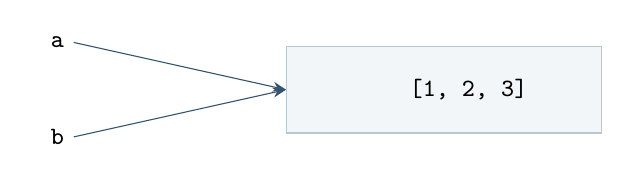
\begin{tikzpicture}[font=\small,>=Stealth]
\node (a) at (0,1) {名称\code{a}};
\node (b) at (0,-0.2) {名称\code{b}};
\node[draw=ThemeBorder,fill=ThemeBack,minimum width=4cm,
 minimum height=1.1cm] (list) at (5,0.4) {同一个列表对象\code{[1, 2, 3]}};
\draw[->,color=ThemeMain] (a.east) -- (list.west);
\draw[->,color=ThemeMain] (b.east) -- (list.west);
\end{tikzpicture}
\end{center}
\term{可变对象}（mutable object）允许改变对象内的内容，例如列表、字典和集合；\term{不可变对象}（immutable object）不能以这种方式改变自身内容，例如整数、字符串和元组。对整数执行\code{x += 1}会计算新整数并重新绑定名称，不是把所有引用原整数的名称一起改成新值。

\code{==}比较值是否相等；\code{is}比较是否为同一个对象。两个独立创建的\code{[1, 2]}通常值相等但身份不同。小整数或字符串的对象复用属于实现细节，不能用\code{is}代替数值或文本相等判断。对\code{None}使用\code{is None}则表达明确的身份检查。

\subsubsection{函数传参为何可能影响调用者}
函数形参同样绑定到实参对象。调用\code{change(values)}不会自动复制列表：
\begin{pycode}
def rebind(values):
    values = [99]


def mutate(values):
    values.append(99)

items = [1, 2]
rebind(items)
print(items)
mutate(items)
print(items)
\end{pycode}
第一次输出\code{[1, 2]}，第二次输出\code{[1, 2, 99]}。\code{rebind}只改变局部名称，\code{mutate}通过引用修改了共享对象。与返回值无关：即使函数没有\code{return}，原地修改也可能已经发生。

\term{副作用}（side effect）指函数除了返回结果外，对外部可观察状态产生的改变，包括修改传入列表、修改全局字典、写文件和打印。副作用并非都错误，\code{fit}更新模型状态就是有意设计的副作用；应明确哪些函数修改什么，不能把评价函数也写成会排序或删除输入记录的隐式修改。

\subsubsection{浅复制与深复制}
\term{浅复制}（shallow copy）创建新外层容器，但内部元素仍引用原来的对象。普通列表的\code{copy()}、\code{list(a)}和\code{a[:]}都可以建立浅复制。\term{深复制}（deep copy）递归复制内部结构，可用标准库\code{copy.deepcopy}。
\begin{pycode}
import copy

rows = [[1, 6], [2, 8]]
shallow = rows.copy()
deep = copy.deepcopy(rows)
shallow[0][1] = 99
shallow.append([3, 10])
print(rows)
print(shallow)
print(deep)
\end{pycode}
输出依次为：
\begin{console}
[[1, 99], [2, 8]]
[[1, 99], [2, 8], [3, 10]]
[[1, 6], [2, 8]]
\end{console}
新外层列表上的追加不影响原外层长度；共享的内层第一行被修改，则两边都能看到。

\begin{center}
\begin{tabularx}{\linewidth}{l Y Y}
\toprule
操作 & 外层身份 & 内层可变对象\\\midrule
\code{b = a} & 相同 & 相同\\
\code{b = a.copy()} & 不同 & 仍可能相同\\
\code{b = copy.deepcopy(a)} & 不同 & 通常递归得到独立副本\\\bottomrule
\end{tabularx}
\end{center}
深复制有时间和空间成本，对文件句柄、外部资源及特殊自定义对象也不能理解为“复制整个运行世界”。若本章训练记录是只含数值的元组，保存\code{tuple(zip(x, y))}已经可以隔离原输入列表的后续增删或数值替换，不需要随意深复制。

\begin{infobox}{例题3.6：二维列表的重复引用}
预测下面代码的结果，并构造两个真正独立的内层列表。
\end{infobox}
\begin{pycode}
rows = [[0, 0]] * 2
rows[0][0] = 7
print(rows)
\end{pycode}
\sol 列表重复运算复制的是其中的引用，两个位置都指向同一内层列表，输出\code{[[7, 0], [7, 0]]}。应写\code{rows = [[0, 0] for _ in range(2)]}，每次循环创建新内层列表。若每一行都用同一个外部列表\code{row}追加，即使使用循环也仍会共享；关键是何时创建对象。

\subsubsection{默认参数与延迟读取的循环变量}
第2章的可变默认参数问题可以用引用解释。\code{def collect(value, bucket=[])}在定义时只创建一次默认列表，后续未提供\code{bucket}的调用会引用它。用\code{None}作默认值，再在函数体中新建列表，才能实现“每次调用独立容器”。若调用者显式传入一个列表，函数仍会按接口修改它。

保存多个预测函数还可能遇到另一种问题：函数执行时才读取外层名称。
\begin{pycode}
functions = []
for k in range(3):
    functions.append(lambda x: x + k)
print([f(10) for f in functions])
\end{pycode}
构建结束后\code{k}为2，三个函数随后调用都读取此时的\code{k}，结果为\code{[12, 12, 12]}。要在每次创建函数时保存当前数值，可以使用默认参数：
\begin{pycode}
functions = []
for k in range(3):
    functions.append(lambda x, k=k: x + k)
print([f(10) for f in functions])
\end{pycode}
结果为\code{[10, 11, 12]}。左侧\code{k}是函数形参，右侧\code{k}在创建时求值。本例保存不可变整数，含义明确；若保存的是可变列表默认值，还需重新检查共享关系。项目比较模型时直接创建不同实例，可以减少保存匿名函数时的这种绑定问题。

\subsection{阅读回溯与检查中间状态}
\subsubsection{从最后一行判断失败类型}
假设\code{run.py}调用\code{metrics.mae}，而函数内部遗漏了非空检查，可能看到如下回溯：
\begin{console}
Traceback (most recent call last):
  File "run.py", line 4, in <module>
    print(mae([], []))
  File "metrics.py", line 3, in mae
    return total / len(actual)
ZeroDivisionError: division by zero
\end{console}
先读最后一行，确定是除以零；再读最近的调用位置，确认分母\code{len(actual)}；随后沿调用链向上追踪为什么传入空列表。修正可能位于指标函数的输入检查，也可能位于前面把数据筛空的代码，应根据接口决定。直接把分母改成\code{len(actual) + 1}会改变指标定义，不能算修复。

回溯所标行号是实际保存文件中的位置。编辑器里未保存的修改尚未执行；运行了同名旧副本时，也可能出现“修改过却没有变化”。应结合\code{__file__}、解释器位置和实际命令确认正在运行哪份程序。

\subsubsection{有问题意识地打印}
调试输出应针对一个假设。若怀疑CSV数值没有转换，应检查字段值的类型；若怀疑划分为空，打印每组长度；若怀疑特征与标签错位，打印带标识的前几条对应记录；若怀疑共享列表，打印\code{a is b}和内部对象的身份关系。
\begin{pycode}
print("source:", data_path)
print("counts:", len(train), len(validation), len(test))
print("first train:", train[:2])
print("label type:", type(train[0]["cost"]).__name__)
\end{pycode}
这一片段需在相应变量建立后执行。先检查\code{train}非空，再访问\code{train[0]}。只打印最终MAE无法分辨数据读取、模型拟合和指标计算分别是否正确。

\term{断点}（breakpoint）让程序暂停在指定位置，以便观察变量并逐步执行。Python内置\code{breakpoint()}通常进入交互调试器；常见操作包括查看变量、单步执行和继续运行。编辑器也可提供图形断点。对本书小程序，先用小输入、状态表和少量打印足以定位大多数问题；避免一次打印整份大数据掩盖关键记录。

\subsubsection{最小可复现示例}
\term{最小可复现示例}（minimal reproducible example）只保留复现同一个错误所需的输入和步骤。若完整项目报告错误，不必一开始就重读全部数据。可以先把触发记录保存成三行CSV，直接调用读取器；若读取正常，再用两条训练记录和一个查询调用模型；最后单独计算一个手算可核对的指标。

缩小问题时必须保留触发条件。广播错误需要保持相关形状，引用错误需要保留共享对象，编码问题需要保留原字符。把所有数据换成简单数字后不再出错，并不证明原程序正确，只说明已删掉某个触发因素。

\begin{infobox}{例题3.7：定位“模型总预测同一个数”}
一个程序的所有预测都是9。给出至少三个可能原因，并分别设计能区分原因的检查。
\end{infobox}
\sol 第一种可能是程序确实选中了训练均值模型，检查对象类型、选择记录和训练均值即可。第二种可能是近邻函数在循环外固定使用第一个查询，应输入相距很远的两个查询，并打印每次距离。第三种可能是保存多个候选时反复引用同一个实例，检查候选对象身份及每次拟合后的状态。还可能是输入列被错误读成常数，应按标识打印原字段和转换后的值。常数输出本身不能唯一证明模型没训练。

\subsection{断言、最小测试与可靠核对}
\subsubsection{assert的用途与限制}
\term{断言}（assertion）写出开发者预期始终成立的内部条件。例如检查输出条数：
\begin{pycode}
assert len(predicted) == len(test)
\end{pycode}
条件为假时会抛出\code{AssertionError}。断言适合教学核对与测试，但在启用优化模式的Python运行中可能被移除。对外部输入的必要检查仍应使用显式条件判断与\code{raise}，不能只依赖断言。
\begin{pycode}
from math import isclose
from metrics import mae

assert isclose(mae([5, 5], [7, 3]), 2.0, rel_tol=0, abs_tol=1e-12)
assert mae([0], [0]) == 0
\end{pycode}
\code{isclose}使用浮点容差。第一个测试包含一正一负残差，能揭示遗漏绝对值的错误；只用\code{[1, 2]}与\code{[2, 3]}，错误的有符号平均也会偶然得到1。核对输入应针对要识别的错误，而非只追求测试数量。

\subsubsection{正常、边界和失败路径}
对MAE，应包含等长正常输入、全零误差、空输入、长度不等和非有限数。对模型，应包含预测前未拟合、两次独立实例、距离同分和输入后来被修改。对文件，应包含错误表头、缺字段、多字段、重复标识和未知集合。每项检查都对应一个明确承诺。

捕获预期异常的最小写法为：
\begin{pycode}
try:
    mae([], [])
except ValueError:
    pass
else:
    raise AssertionError("empty inputs were not rejected")
\end{pycode}
这里的\code{pass}表示测试已经收到所要求的异常，不是项目运行时忽略失败。若没有报错，\code{else}让测试失败；若报了其他类型的异常，也应暴露出来，因为那并不符合约定。

\term{单元测试}（unit test）核对一个较小组件；\term{集成测试}（integration test）核对多个组件连接后的行为。分别检查读取器和模型，不能替代检查整条流程是否仍将正确标签交给指标。反过来，只核对最终MAE也可能让两个错误彼此抵消。完整项目保留少量两类检查。

\subsubsection{使用标准库unittest}
\code{unittest}是标准库测试工具，以方法组织测试，并报告哪些检查失败。本章\code{test_project.py}包含以下形式：
\begin{pycode}
import unittest
from metrics import mae

class MetricTests(unittest.TestCase):
    def test_hand_value(self):
        self.assertAlmostEqual(mae([5, 5], [7, 3]), 2.0)

    def test_empty(self):
        with self.assertRaises(ValueError):
            mae([], [])

if __name__ == "__main__":
    unittest.main()
\end{pycode}
\code{TestCase}提供核对方法，\code{test_}开头的方法被识别为测试。\code{assertAlmostEqual}检查浮点结果，\code{assertRaises}检查是否抛出指定异常。此处继承仅用于沿用测试工具已定义的功能，无需先设计复杂类层次。命令\code{python3 test_project.py}会运行测试并打印通过数量。

测试不能证明所有可能输入都正确，但可以固定已经明确的规则，帮助修改代码后发现退步。若把预期值写成与被测函数完全相同的计算，就容易共同犯错；本章优先采用手算小例、独立实现对照和特定失败输入。

\subsection{实验3.1：对象变化与文件往返}
入口为\code{配套实验/ch03_objects.py}，仅依赖Python标准库。程序不要求输入个人文件，文件实验在自动建立的临时目录中进行，结束后清理。实验同时核对三个问题：哪些修改会穿过共享引用；怎样在每次调用时创建独立列表；JSON写入再读回是否保持预期数据。

开始前手工画出\code{rows}、\code{alias}、\code{shallow}、\code{deep}指向的外层和内层对象。核心操作为：
\begin{pycode}
rows = [[1, 6], [2, 8]]
alias = rows
shallow = rows.copy()
deep = copy.deepcopy(rows)
alias.append([3, 10])
shallow[0][1] = 99
\end{pycode}
\code{alias.append}修改原外层列表，所以\code{rows}增加一行，\code{shallow}的长度仍为2。第二次操作修改共享内层第一行，所以\code{rows}和\code{shallow}的费用都变为99。\code{deep}保存的原始两行不变。

在项目的配套实验目录运行：
\begin{console}
python3 ch03_objects.py
\end{console}
主要预期输出为：
\begin{console}
rows: [[1, 99], [2, 8], [3, 10]]
shallow: [[1, 99], [2, 8]]
deep: [[1, 6], [2, 8]]
identity: True False True False
fresh: [1] [2]
captured: [10, 11, 12]
round trip: 3 教学数据
caught: ValueError
all checks passed
\end{console}
身份比较依次核对别名与原列表、浅复制与原列表、浅复制第一行与原第一行、深复制第一行与原第一行。结果应精确一致；本实验没有近似数值计算。

文件往返部分使用\code{TemporaryDirectory}作为上下文管理器。进入时创建临时目录，将字典写入\code{report.json}再读回；退出时删除本实验临时目录。这是标准库管理临时资源的实例，不能将它替换为随意删除原始数据目录。

修改任务依次进行，每次从原版恢复：把\code{shallow}改为深复制，预测第一行还会不会互相影响；把默认参数改成\code{bucket=[]}，连续调用观察累积；去掉\code{lambda}中的\code{k=k}，预测三个输出；把JSON中的整数改成元组\code{(1, 2)}，读回后核对类型。最后一个任务应得到列表，说明数据往返不保证保留所有Python类型。

\subsection{实验3.2：组织可复现的预测小程序}
\subsubsection{目录、输入与流程约定}
入口为\code{配套实验/ch03_project/main.py}。\term{可复现}（reproducible）在本章指：给定同一代码、数据、环境和流程规则，可以从头得到一致的预测和评价结果。它不等同于模型对未来数据一定可靠，也不要求不同机器生成完全相同的耗时或临时路径。
\begin{console}
ch03_project/
    main.py
    io_utils.py
    models.py
    metrics.py
    test_project.py
    data/parcels.csv
    results/summary.json
    results/predictions.csv
\end{console}
\code{main.py}协调流程；\code{io_utils.py}负责严格读取与结果写出；\code{models.py}保存模型类；\code{metrics.py}提供MAE；\code{test_project.py}核对规则。结果文件由运行生成。依赖关系由入口指向各组件，组件不导入入口，导入模块不启动实验。

数据有12条，训练、验证、测试各4条，划分直接由CSV的\code{split}列指定。本章不重新随机划分，因此没有用一个随机种子代替数据记录的必要。数据如下，重量和费用均为教学构造值。
\begin{center}
\begin{tabular}{c l l}
\toprule
集合 & 重量（千克） & 费用（元）\\\midrule
训练 & 1，2，3，4 & 6，8，10，12\\
验证 & 1.2，2.2，3.2，3.8 & 6.4，8.4，10.4，11.6\\
测试 & 1.4，2.6，3.4，4.5 & 6.8，9.2，10.8，13.0\\\bottomrule
\end{tabular}
\end{center}
候选为训练均值模型和单近邻模型；按最小验证MAE选择，同分时取声明顺序靠前者。单近邻距离同分时取训练记录中靠前者。选定后不把验证集合并重训，直接评价已选模型；这样能明确追踪每次拟合到底使用哪些标签。其他项目可以另定重训协议，但必须记录并保持一致。

\subsubsection{严格读取与保持记录对齐}
读取器先验证\code{reader.fieldnames}等于预期表头。每条记录转换前检查字段数、非空唯一标识和合法集合名。对\code{DictReader}，多出的字段可能对应键\code{None}，缺少的字段可能对应值\code{None}；因此完整读取器有如下检查：
\begin{pycode}
if None in row or any(v is None for v in row.values()):
    raise ValueError(f"row {line}: wrong field count")
\end{pycode}
通过检查后再解析\code{float}，验证有限、非负，最后建立规范字典。这一过程先保证数据结构，再保证字段意义，不能只看能否运行除法。完整实现保存在\code{io_utils.py}；讲义中的短片段用于说明该检查的原因，运行时使用完整入口。

训练输入和标签必须从同一记录顺序提取：
\begin{pycode}
def columns(records):
    return ([row["weight"] for row in records],
            [row["cost"] for row in records])
\end{pycode}
这里两次遍历同一个未被修改的记录列表，因此位置对应。更换顺序或筛选时，应对整条记录操作，而非分别排序重量和费用。唯一标识只能揭示某些重叠，不能证明不同标识没有复制内容；真实数据仍需按第1章协议检查来源与重复样本。

\subsubsection{用相同接口比较两个模型}
均值模型的\code{fit}保存\code{sum(y) / len(y)}。单近邻模型的\code{fit}保存\code{tuple(zip(x, y))}，\code{predict}逐个查询最近训练记录：
\begin{pycode}
return [min(self.records_, key=lambda row: abs(row[0] - q))[1]
        for q in x]
\end{pycode}
这一片段位于完成拟合状态和输入检查后的方法内部。\code{min}在同分时选第一次遇到的记录；\code{[1]}取得费用。与第1章完整排序相比，单个近邻只需扫描找到最小值，无需把所有距离排序。对 $n$ 条训练记录、$m$ 个查询，时间为 $O(mn)$；保存训练记录需要 $O(n)$ 空间，保存输出需要 $O(m)$。这里 $O$ 表示随输入规模增长的量级，不表示实际秒数。

入口中每个候选都创建新实例：
\begin{pycode}
factories = {"mean": MeanRegressor, "nearest": NearestRegressor}
models = {}
scores = {}
for name, factory in factories.items():
    model = factory().fit(x_train, y_train)
    models[name] = model
    scores[name] = mae(y_val, model.predict(x_val))
selected = min(scores, key=scores.get)
\end{pycode}
\code{factory}在这里是类对象，\code{factory()}创建对应实例。两个字典分别保存模型和验证分数，不把模型对象与浮点分数混在一起。\code{scores.get}作为比较函数，让\code{min}按键对应的分数选择；字典的插入顺序对应已声明的候选顺序。

读取器会一次读入文件全部字段，但候选拟合只接收训练标签，候选选择只接收验证指标。文件中存有测试标签不自动构成泄漏，关键是这些标签是否影响训练或选择；本章按代码依赖限制其用途。真实项目也可把最终测试标签交给独立评价程序管理。

\subsubsection{手算验证选择与最终评价}
训练均值为 $(6+8+10+12)/4=9$。在验证集，四个绝对误差为2.6、0.6、1.4、2.6，因此MAE为1.8。单近邻分别找到重量1、2、3、4，预测6、8、10、12，绝对误差均为0.4，MAE为0.4，应选择单近邻。

测试只对选定模型作最终报告，同时保留预先声明的均值基线作比较：
\begin{center}
\begin{tabular}{ccccc}
\toprule
重量 & 真实费用 & 单近邻预测 & 单近邻绝对误差 & 基线绝对误差\\\midrule
1.4 & 6.8 & 6 & 0.8 & 2.2\\
2.6 & 9.2 & 10 & 0.8 & 0.2\\
3.4 & 10.8 & 10 & 0.8 & 1.8\\
4.5 & 13.0 & 12 & 1.0 & 4.0\\\bottomrule
\end{tabular}
\end{center}
单近邻测试MAE为 $(0.8+0.8+0.8+1.0)/4=0.85$；均值基线为 $8.2/4=2.05$。4.5超过训练重量范围，单近邻仍返回边界费用12；这体现近邻方法的外推限制。该数据构造得十分规则，结果不能用于推断真实物流业务表现。

\subsubsection{运行、保存与再次运行}
在配套实验目录执行：
\begin{console}
python3 ch03_project/main.py
python3 ch03_project/test_project.py
\end{console}
也可从其他目录用入口的绝对路径运行。程序应输出：
\begin{console}
counts: {'train': 4, 'validation': 4, 'test': 4}
validation mean: 1.800000
validation nearest: 0.400000
selected: nearest
test predictions: [6.0, 10.0, 10.0, 12.0]
test MAE: 0.850000
test baseline MAE: 2.050000
saved: results/summary.json, results/predictions.csv
\end{console}
第二个命令应报告5项测试通过。报告数字按六位小数显示，内部计算允许约 $10^{-12}$ 的绝对误差。每条预测、集合计数和被选名称应一致，不把打印舍入差异解释为模型改变。

JSON记录Python版本、数据文件的SHA-256摘要、集合数量、候选顺序、选择规则、是否重训、验证分数和最终指标。\term{摘要}（hash digest）把文件内容映射为定长标识，有助于判断两次运行是否使用相同字节；它不证明数据真实、标签正确或划分合理。仅修改CSV换行也会改变摘要，但模型数值可能仍相同。

预测CSV保存标识、真实值、预测值与逐条绝对误差。再次运行会替换同名结果；代码与数据不变时，关键数值应相同。跨Python版本的版本字段自然不同，JSON字节完全相同不是本章复现要求。需要保留多次结果时，应复制到明确编号目录，并同时保留对应代码与输入。

\subsubsection{有控制地修改与故障注入}
从原始数据副本开始，每次只改一个因素，运行后恢复原版。
\begin{enumerate}
\item 把某重量改为\code{nan}，应在读取阶段失败并提示记录位置，不生成新的完整成功结果；旧输出若仍存在，也不能当作本次成功证据。
\item 把一条验证记录的标识改成训练标识，应拒绝重复。将集合名称拼成\code{validaton}，应拒绝未知集合。
\item 从其他工作目录启动入口，数值应与原版一致；若改成裸相对数据路径，应能复现路径错误，再恢复正确定位。
\item 将第一条训练费用6改为10，先手算两候选验证分数，再运行。不能根据测试分数把该修改说成真实改进。
\item 单独对重量100作预测，应得到12；该输入没有真实标签时，不并入MAE。解释为什么程序能给出数值并不保证外推可靠。
\end{enumerate}
第4项的均值变为10，验证MAE为1.8；单近邻验证误差为3.6、0.4、0.4、0.4，MAE为1.2，仍选单近邻。修改后最终测试误差变成3.2、0.8、0.8、1.0，MAE为1.45。该手算用于核对流程传播，不能用最终测试数值倒推应怎样修改训练数据。

\subsection{知识联系与自检}
程序中的三类联系需要分别理解。模块依赖说明代码从哪里取得；对象引用说明哪些名称共享状态；数据依赖说明哪些记录影响模型和选择。正确的导入结构不能自动防止标签泄漏，独立的对象也不能自动防止读错文件。

第2章函数的输入输出约定在本章扩展为模块接口和模型方法；列表切片的浅复制与本章的内部共享相连；第1章的训练、验证、测试在入口中表现为不同的数据传递。第4章增加数组以后，除这些要求外，还必须核对轴、形状和共享内存。

自检时应能回答：为什么脚本可导入却读不到数据；为什么\code{b = a}不是模型快照；为什么捕获错误后填0会改变任务；为什么空输入应由显式检查拒绝；为什么一个测试应包含正负残差；为什么相同种子不能代替保存数据版本。回答应举出具体语句或输入，而非只复述术语。

\subsection{分层习题}
以下编号为3.1--3.14。代码题先写预期状态，再运行核对；文件题使用自己建立的临时数据，不修改原始教学数据。
\begin{enumerate}[label=\textbf{3.\arabic*}]
\item \textbf{概念。}区分脚本、模块、包和第三方依赖；说明\code{from metrics import mae}后为什么不能直接推断名称\code{metrics}可用。
\item \textbf{执行分析。}在例题3.1中将第一行打印移入\code{main}，直接运行和首次导入各输出什么？重复导入为什么通常不再次执行顶层语句？
\item \textbf{路径。}工作目录为\code{/tmp}，源文件在项目目录中。对以下两种定位写出实际指向的位置。
\begin{console}
源文件：/tmp/project/main.py
路径甲：Path("data/a.csv")
路径乙：Path(__file__).resolve().parent / "data" / "a.csv"
\end{console}
\item \textbf{文件。}解释\code{"r"}、\code{"w"}、\code{"a"}的区别，为什么打开原始数据时不能误用\code{"w"}？\code{with}解决什么问题，不能保证什么？
\item \textbf{输入验证。}实现\code{parse_nonnegative(text)}，接受可转为有限非负浮点数的文本，其他情况抛\code{ValueError}。核对\code{"0"}、\code{"nan"}、\code{"inf"}、\code{"-1"}与\code{"missing"}。
\item \textbf{引用。}假定已导入\code{copy}，执行以下语句后写出四个变量的值。
\begin{pycode}
a = [[1, 2], [3, 4]]
b = a
c = a.copy()
d = copy.deepcopy(a)
b.append([5, 6])
c[0][0] = 9
\end{pycode}
\item \textbf{副作用。}比较函数内部\code{values = sorted(values)}与\code{values.sort()}对调用者列表的影响。设计一个输入和检查区分两者。
\item \textbf{类与状态。}为什么均值模型未拟合标记用\code{None}，而不使用0？若\code{a}和\code{b}引用同一模型，连续拟合会有什么后果？给出独立创建的写法。
\item \textbf{绑定。}三个函数在循环中通过\code{lambda x: x + k}保存，循环结束再调用得到什么？改为保存当前整数\code{k}，并解释默认参数求值时机。
\item \textbf{异常与测试。}有人用\code{except Exception: return 0}包装整个MAE函数，称“任何输入都不报错”。指出这怎样破坏接口，并写一个检查空输入必须报错的最小测试。
\item \textbf{项目手算。}实验3.2将第一条训练费用改为10，其他不变。计算两候选验证MAE、选定模型和测试MAE，说明哪些结果必须重新生成。
\item \textbf{JSON。}字典\code{{"pair": (1, 2), "missing": None}}经过JSON写入与读回后，各值是什么类型？为何不应直接保存模型实例？
\item \textbf{故障定位。}项目报\code{KeyError: 'cost'}。给出应依次检查的三个具体位置；为什么不应直接改成\code{row.get("cost", 0)}？
\item \textbf{综合实验。}从项目目录与另一目录分别运行实验3.2，再运行其测试。核对预测文件、数据摘要和指标；列出报告中哪些字段用于复现、哪些条件仍不足以证明真实泛化。
\end{enumerate}

\subsection{习题参考答案}
\subsubsection*{3.1--3.4：组织、路径与文件}
\textbf{3.1}\quad 脚本强调作为入口执行的文件；模块强调可导入的代码单元，同一文件可以兼具两种用途；包组织多个模块；第三方依赖是需要安装到解释器环境中的外部代码。\code{from metrics import mae}只把指定名称绑定到当前名称空间，不同时绑定\code{metrics}；需用\code{import metrics}才能按模块前缀访问。

\textbf{3.2}\quad 移入后直接运行输出\code{loading}与\code{running}，首次导入不输出文字。普通重复导入通常复用进程中已缓存模块；重启解释器后会重新建立模块。入口保护控制是否调用\code{main}，缓存则控制普通重复导入是否重新初始化，两个机制不同。

\textbf{3.3}\quad 前者按当前工作目录解释为\code{/tmp/data/a.csv}；后者以源文件父目录为起点，指向\code{/tmp/project/data/a.csv}。\code{resolve}解析符号链接，本题假定没有符号链接影响。两者不能仅从路径字符串都含\code{data}就视为相同。

\textbf{3.4}\quad \code{"r"}读取且文件应存在；\code{"w"}写入并在打开时截断原内容；\code{"a"}在末尾追加，重复运行可能重复记录。\code{with}保证按上下文管理规则退出，普通文件会被关闭；不能保证写入内容符合任务，也不能保证多个文件在故障时全部完整写入。

\subsubsection*{3.5--3.9：验证、引用与对象}
\textbf{3.5}\quad 先转换，再检查有限与非负；不能以真假判断代替非负检查。
\begin{pycode}
import math

def parse_nonnegative(text):
    try:
        value = float(text)
    except ValueError as exc:
        raise ValueError("not a number") from exc
    if not math.isfinite(value) or value < 0:
        raise ValueError("expected finite nonnegative number")
    return value
\end{pycode}
\code{"0"}返回0.0，其余四项抛\code{ValueError}。本题接口接受文本，不承诺任意Python对象都被统一转为同一错误。配套\code{ch03_solutions.py}核对这些输入。

\textbf{3.6}\quad 四个名称的值为：
\begin{console}
a, b: [[9, 2], [3, 4], [5, 6]]
c:    [[9, 2], [3, 4]]
d:    [[1, 2], [3, 4]]
\end{console}
追加通过共享外层作用于\code{a}和\code{b}；第一项修改通过共享内层作用于\code{a}、\code{b}、\code{c}；\code{d}在两次操作前已递归复制。

\textbf{3.7}\quad 函数内\code{values = sorted(values)}建立新排序列表并重绑局部名称，调用者列表不变；\code{values.sort()}原地排序，调用者看到变化。以\code{items = [3, 1, 2]}分别传入，调用后核对原列表与\code{[3, 1, 2]}是否相等即可。若原列表本来已排序，这个输入就无法揭示两者行为差异。

\textbf{3.8}\quad 均值0是合法训练结果，真假判断会把它误当成未拟合。\code{None}明确标记缺少训练状态。同一模型被两个名称引用时，后一次拟合覆盖前次状态；独立写\code{a = MeanRegressor()}与\code{b = MeanRegressor()}，再分别拟合。若用字典保存比较结果，也应每次创建新实例。

\textbf{3.9}\quad 循环结束\code{k=2}，原版三个函数对10都返回12。改成\code{lambda x, k=k: x + k}后，创建时分别保存0、1、2，对10返回10、11、12。这里默认值在函数对象创建时求值，不是在后续每次调用时重新读取循环变量。

\subsubsection*{3.10--3.14：失败路径与复现}
\textbf{3.10}\quad 返回0把输入错误、程序缺陷和真正零误差合并为一个无法区分的结果，可能让错误方案看起来最好。可使用本章的\code{try/except/else}最小测试，或在\code{unittest.TestCase}方法内写：
\begin{pycode}
with self.assertRaises(ValueError):
    mae([], [])
\end{pycode}
测试中捕获预期异常是核对失败路径；实际评价中忽略异常并给出零分则改变接口含义。

\textbf{3.11}\quad 训练费用变为10、8、10、12，均值10。验证均值误差3.6、1.6、0.4、1.6，总和7.2，MAE为1.8。单近邻验证误差3.6、0.4、0.4、0.4，总和4.8，MAE为1.2，选单近邻。测试预测为10、10、10、12，误差3.2、0.8、0.8、1.0，MAE为1.45。数据摘要、验证分数、选择报告和逐条预测应一起更新。用测试分数选择是否保留该修改会违反原协议。

\textbf{3.12}\quad \code{pair}读回为列表，\code{missing}读回为\code{None}。JSON保留常用数据结构，不保存任意类的方法、运行资源或全部类型身份。模型实例应选取必要配置与训练状态按明确格式保存；本章只保存结果报告，不承诺可从报告恢复模型。

\textbf{3.13}\quad 先检查原CSV表头是否真有\code{cost}，包括两端空格与大小写；再检查读取器构造字典时是否换名或漏字段；最后检查报错行变量是否仍是预期记录，而不是另一种字典。默认0会把缺字段变成测量值，掩盖格式错误，并可能改变训练目标或评价标签。应在读取边界拒绝不合约定的数据。

\textbf{3.14}\quad 两种启动位置应给出相同集合数量、模型选择、预测与关键指标；数据未变时摘要一致。记录Python版本、代码版本或副本、数据内容、划分、候选顺序和同分规则，才能解释复现条件。本项目还需保留主源及配套代码的对应版本。即使这些条件满足，也只能复现教学实验，不能保证未来分布、标签质量和真实业务代价与该数据相同。

\subsection{本章小结}
模块给代码划分名称和依赖边界，路径给文件确定位置，数据格式与验证确定输入含义。类把训练状态和预测方法连接起来；引用决定状态是否共享，复制决定哪些层次独立。调试通过回溯、中间状态和最小输入寻找原因，测试把已明确的规则固定为可重复检查。

实验3.2将这些机制落实为可从头运行的预测流程。结果是否可复现，要检查代码、数据、环境和选择协议；评价是否可信，还要回到第1章对信息可用性、划分和泛化条件的要求。
\chapterpage{NumPy与向量化计算}\label{ch:numpy}
\begin{infobox}{先修知识、学习目标与本章位置}
本章需要第2章的循环、列表和函数，以及第3章的导入、对象、引用与调试。矩阵运算只用到按行列取值、乘积求和和平均数，所需含义在本章补充，第6章再系统复习线性代数。

学习后应能解释数组的类型、轴和形状；区分索引、切片、视图与复制；逐轴核对广播和矩阵乘法；用归约与向量化替代逐样本循环；控制随机数并检查浮点结果；从头完成一个无预处理泄漏的数值实验。
\end{infobox}
第2章用循环逐条计算预测、残差与平均误差，这种写法直接反映计算过程。数据量增加以后，可以把规则相同的操作交给专门的数值库一次完成。\term{NumPy}（Numerical Python）是Python科学计算中的基础数组库，提供多维数组及其运算。NumPy数组也会遇到逻辑错误：程序能运算，只说明类型与形状在规则上兼容，不说明每一行仍对应正确样本。

本章把数组理解为带有形状与数据类型的数值容器。先逐项说明它与列表的不同，再建立逐元素运算、归约、广播和矩阵乘法的联系。所有维度推导都回到元素下标，避免只凭代码短或输出形状合理就判断正确。

\subsection{安装、导入与数组的用途}
\subsubsection{让解释器与依赖处于同一环境}
NumPy是第三方依赖，需安装到实际运行脚本的Python环境中。按第2章建立并激活虚拟环境后，可在普通终端执行：
\begin{console}
python3 -m pip install numpy
python3 -c "import numpy as np; print(np.__version__)"
\end{console}
Windows按第2章将\code{python3}换为相应启动命令。\code{-m pip}让所选解释器运行包安装工具，减少把包装到另一个解释器的情况。若已安装且能导入，无需重复安装。网络不可用时可使用已经提供NumPy的环境，本书实验不依赖下载数据。

代码中采用惯用别名：
\begin{pycode}
import numpy as np

values = np.array([1.0, 2.0, 3.0])
print(values)
print(type(values))
\end{pycode}
输出数值数组和其类型\code{numpy.ndarray}。\code{np}只是\code{numpy}的当前名称，不是Python内置关键字；\code{ndarray}表示多维数组类型。后文代码框未重复导入时，均以此前已执行\code{import numpy as np}为前提。

配套实验在Python 3.12与NumPy 2.3.5环境实际核对。基础接口不依赖特定硬件；复现时应记录自己的版本，而不是只写“已安装Python”。安装命令不固定后续所有版本行为，项目要长期复现时应同时保留已核对的依赖版本。

\subsubsection{列表运算与数组运算不同}
\begin{pycode}
items = [1, 2, 3]
array = np.array(items)
print(items * 2)
print(array * 2)
print(items + items)
print(array + array)
\end{pycode}
列表乘2得到\code{[1, 2, 3, 1, 2, 3]}，表示序列重复；数组乘2得到\code{[2 4 6]}，表示每个元素乘2。列表相加连接序列，数组相加执行逐位置加法。NumPy显示数组时通常不在数字间添加逗号，显示格式不意味着它变成另一种数学对象。

\term{向量化}（vectorization）在本章指把逐元素或逐样本的规则表达为数组级操作，使主要循环由数值库执行。它没有消除底层循环，而是减少Python层逐项调度，并利用面向数组的实现。列表推导式虽然简短，仍然主要是Python逐项执行，不等于NumPy向量化。

NumPy不自动把所有工作放到\term{GPU}（graphics processing unit，图形处理器）上，本章标准数组在\term{CPU}（central processing unit，中央处理器）上计算。深度学习中的设备与张量将在第25章讲解；数组代码正确与使用哪种硬件是两个问题。

\subsection{数组形状、轴与统一的数据约定}
\subsubsection{shape、ndim、size和dtype}
\term{形状}（shape）给出每个\term{轴}（axis）的长度；\term{维数}在数组语境中常指轴的个数，用\code{ndim}表示；\code{size}表示总元素数量；\code{dtype}表示元素数据类型。四者承担不同工作。
\begin{pycode}
X = np.array([[1.0, 2.0, 3.0], [4.0, 5.0, 6.0]])
print(X.shape)
print(X.ndim)
print(X.size)
print(X.dtype)
\end{pycode}
分别得到\code{(2, 3)}、2、6与\code{float64}。\code{shape}是元组；\code{(3,)}表示单轴长度3，逗号不可省略；零维数组形状为\code{()}。若形状为 $(s_0,\ldots,s_{r-1})$，总元素数为各长度的乘积，轴数为 $r$。对矩阵形状 $(n,d)$，\code{len(X)}只给出第一轴长度 $n$，不等于总元素数 $nd$。

\begin{center}
\begin{tabularx}{\linewidth}{l c Y}
\toprule
创建方式 & 形状 & 结构含义\\\midrule
\code{np.array(3.0)} & \code{()} & 零维数组，含一个数\\
\code{np.array([1, 2, 3])} & \code{(3,)} & 一维数组，没有独立行轴与列轴\\
\code{np.array([[1, 2, 3]])} & \code{(1, 3)} & 二维数组，一行三列\\
\code{np.array([[1], [2], [3]])} & \code{(3, 1)} & 二维数组，三行一列\\\bottomrule
\end{tabularx}
\end{center}
同样三个数，可以有不同形状。数学中的列向量常写成 $3\times1$，NumPy中的长度3一维数组却不自动带有“列”方向。\code{w.T}对一维数组仍为一维，必须明确增加轴才能得到二维列数组。

\subsubsection{样本轴与特征轴}
本书对普通表格数值数据采用
\[
 X\in\mathbb R^{n\times d},\qquad
 X_{ij}=\text{第 $i$ 个样本的第 $j$ 个特征}.
\]
数学下标在推导中通常从1开始，Python索引从0开始，程序位置\code{X[0, 0]}对应数学 $X_{11}$。$n$ 为样本数，$d$ 为每个样本的特征数，\code{X.shape == (n, d)}。轴0沿样本变化，轴1沿特征变化。

例如两件包裹分别有三个已数值化特征，数组可以为
\[
 X=\begin{pmatrix}1&2&3\\4&5&6\end{pmatrix}.
\]
第一行是一个样本，不是一个特征的全部测量。若把矩阵转置为 $3\times2$，数值总数不变，但样本与特征的解释互换。形状必须与语义一起写，不能只写“这是一个二维数组”。

\begin{infobox}{注意：数组维数与特征维数}
100个样本、每个样本有20个特征，可表示为形状\code{(100, 20)}的二维数组；特征空间则是20维。说“数据是20维”与说“数组有两个轴”并不矛盾，它们描述不同事物。后续一批图像可能有样本、高度、宽度、通道等轴，仍需逐轴解释。
\end{infobox}

\subsubsection{reshape、增加轴与转置}
\code{reshape}按指定顺序重新组织元素，要求总元素数量不变：
\begin{pycode}
a = np.arange(6)
print(a.reshape(2, 3))
print(a.reshape(3, 2))
print(a.reshape(-1, 1).shape)
\end{pycode}
\code{arange(6)}给出0至5；默认按行顺序填入。前两次分别得到两行三列和三行两列；\code{-1}表示由其他轴长度推算该轴，最后形状为\code{(6, 1)}，最多只能有一个待推算轴。没有依据地\code{reshape}可能让一个样本的特征散落到多行，即使元素数正确仍破坏数据含义。

增加长度为1的轴可用\code{None}或\code{np.newaxis}：
\begin{pycode}
w = np.array([1.0, 2.0, 3.0])
print(w[:, None].shape)
print(w[None, :].shape)
print(w.T.shape)
\end{pycode}
依次为\code{(3, 1)}、\code{(1, 3)}和\code{(3,)}。二维数组\code{X.T}交换两个轴；\code{reshape(3, 2)}与\code{X.T}一般不是同一运算。对前面的 $X$，转置为 $\bigl(\begin{smallmatrix}1&4\\2&5\\3&6\end{smallmatrix}\bigr)$，而直接重排为 $\bigl(\begin{smallmatrix}1&2\\3&4\\5&6\end{smallmatrix}\bigr)$。

\code{reshape}可能返回共享数据的视图，也可能因为内存布局而复制，不能一律当成独立副本。需要独立数据时显式\code{copy()}。\code{squeeze}可去除长度为1的轴，但在单样本批次中不加选择地挤压，可能把样本轴也去掉；优先明确指定要处理的轴。

\subsection{数据类型、数组创建与数值范围}
\subsubsection{同一dtype与固定宽度}
普通数值数组的元素共用一个\code{dtype}。\code{float64}通常以64位表示浮点数，\code{float32}通常以32位表示；\code{int64}表示固定宽度整数；\code{bool}表示布尔值。位数影响可表示范围、精度和内存，不表示小数点后固定保存64或32位。
\begin{pycode}
counts = np.array([1, 2, 3], dtype=np.int64)
weights = counts.astype(np.float64)
print(weights.dtype)
print(weights.itemsize, weights.nbytes)
\end{pycode}
\code{astype}在这里转换并建立新数组；\code{itemsize}为每元素字节数，\code{nbytes}为元素数据所占字节数。三个\code{float64}元素共24字节，不含Python对象元数据等额外成本。约百万个\code{float64}元素需要约800万字节，仅是数组数据本身的量级估算。

整数数组里写小数不会自动把整个数组改为浮点类型：
\begin{pycode}
a = np.array([1, 2], dtype=np.int64)
a[0] = 1.9
print(a)
\end{pycode}
结果为\code{[1 2]}，小数部分被截去。用于平均、标准化与模型系数的数组应从开始就明确采用合适浮点类型，而不是等发现小数丢失后再转换。

Python整数可按需要扩大表示，但NumPy固定宽度整数可能溢出。例如两个\code{uint8}数组\code{[250]}和\code{[10]}相加，结果按其范围回绕为\code{[4]}。图像像素常见0--255整数，直接做差或平方可能在计算前就出错。应先把输入转换成浮点，再相减或平方；在错误计算以后才转浮点，不能恢复已经丢失的信息。

\subsubsection{规则数组与对象数组}
\code{np.array([[1, 2], [3, 4]])}有规则矩形结构；\code{[[1, 2], [3]]}各行长度不等，不能直接作为常规二维数值数组。混入字符串可能使数组转为字符串类型，后续加减不再具有原数值意义。

\code{dtype=object}可以装入一般Python对象，但会回到逐对象操作，也带来第3章的内部可变对象共享问题。本章聚焦规则数值数组，不用对象数组绕开结构错误。数组的\code{copy()}复制数值缓冲区；若数组元素本身是对象引用，它不自动深复制这些对象。

\subsubsection{zeros、ones、arange与linspace}
\begin{pycode}
print(np.zeros((2, 3)))
print(np.ones((1, 3)))
print(np.arange(1, 7, 2))
print(np.linspace(0.0, 1.0, 5))
\end{pycode}
前两者创建指定形状的全0、全1数组；\code{arange}按步长生成并通常不含终点，得到1、3、5；\code{linspace}指定点数，默认包含两端，得到0、0.25、0.5、0.75、1。需要固定数量的等距浮点点时，\code{linspace}比依赖浮点步长恰好落在终点更清楚。

\code{np.full((n,), value)}创建指定值填充的数组，适合均值基线。\code{np.empty}分配数组但不把元素初始化为约定数值，其内容不能在完整赋值之前使用。\code{zeros_like(X)}沿用\code{X}的形状和通常的数据类型；若\code{X}是整数，不能假定新数组就适合存标准化小数。

\subsection{索引、切片、布尔筛选与共享内存}
\subsubsection{二维索引与保留轴}
\begin{pycode}
X = np.array([[1., 2., 3.], [4., 5., 6.]])
print(X[1, 2])
print(X[0].shape)
print(X[:, 1].shape)
print(X[:, 1:2].shape)
print(X[0:1, :].shape)
\end{pycode}
依次为6.0、\code{(3,)}、\code{(2,)}、\code{(2, 1)}和\code{(1, 3)}。单个整数索引选定该轴的一项并去除该轴；切片即使只选一项也保留该轴。二维写法\code{X[i, j]}直接说明两个轴的索引，通常比连续\code{X[i][j]}更容易核对。

\begin{infobox}{例题4.1：同一列的两种形状}
\code{X.shape == (5, 3)}。预测\code{X[:, 0]}、\code{X[:, 0:1]}、\code{X[0, :]}、\code{X[0:1, :]}的形状，并说明哪些仍是二维数组。
\end{infobox}
\sol 依次为\code{(5,)}、\code{(5, 1)}、\code{(3,)}、\code{(1, 3)}。第二、四项仍有两个轴。若模型接口要求 $n\times d$ 输入，一个样本也应保留为\code{(1, d)}；若指标要求一维标签，就应有意取成\code{(n,)}，而非随意保留或去除轴。

\subsubsection{基本切片的视图与显式复制}
\term{视图}（view）是共享同一底层数据的数组表示，可以有不同形状、偏移和步长。数值数组的基本切片通常给出视图，与第2章列表切片建立新外层列表的行为不同。
\begin{pycode}
a = np.array([[1., 2.], [3., 4.]])
view = a[:, :1]
independent = a[:, :1].copy()
view[0, 0] = 99
independent[1, 0] = -1
print(a)
print(independent)
print(np.shares_memory(a, view))
\end{pycode}
原数组变为\code{[[99., 2.], [3., 4.]]}；独立副本为\code{[[1.], [-1.]]}；共享检查为真。\code{view is a}虽为假，两者仍共享数据；身份不同不能推出数据互相独立。

\code{a = np.asarray(source)}用于取得数组表示；若输入已经是兼容类型的数组，它可能直接返回同一对象。需要保护调用者输入时，不应只写\code{asarray}就假定复制完成。\code{np.array(source, copy=True)}或转换后的\code{copy()}可以明确请求独立数值缓冲区。

视图可避免复制大块数据，但也会延长底层数据的存活。例如从很大的数组取得一个小切片，若仍引用原缓冲区，保留小切片可能继续占着大块内存。是否复制要根据共享语义与内存用途决定，不能一律认为“视图总更好”。

\subsubsection{整数数组索引与布尔筛选}
\term{高级索引}（advanced indexing）包括整数数组和布尔数组等形式。读取时通常产生新数组：
\begin{pycode}
a = np.array([[1., 2.], [3., 4.], [5., 6.]])
picked = a[[0, 2]]
picked[0, 0] = 99
mask = a[:, 0] >= 3
print(mask)
print(a[mask])
print(a[0, 0])
\end{pycode}
布尔掩码为\code{[False True True]}，筛选后保留后两行；原\code{a[0, 0]}仍为1.0。\term{掩码}（mask）在这里是决定保留哪些位置的布尔数组。多个条件使用\code{&}、\code{|}与\code{~}并分别加括号，例如\code{(a[:, 0] >= 3) & (a[:, 1] < 6)}。Python的\code{and}不是逐元素数组逻辑操作。

直接赋值\code{a[mask] = 0}会修改原数组，因为它以原数组为赋值目标；不能根据“读取高级索引得到副本”推断这句也不修改原数组。\code{a[mask][:, 0] = 0}则先得到临时副本，再改副本，往往不改变\code{a}。避免依赖连续索引的隐含中间对象，直接指定清楚的赋值位置。

\code{X[[0, 1], [1, 2]]}按位置配对，取\code{X[0, 1]}和\code{X[1, 2]}，不是取两行两列的全部交叉组合。若要子矩阵，可以写\code{X[np.ix_([0, 1], [1, 2])]}。复杂索引先在小矩阵上核对实际值，再用于数据集。

\subsection{逐元素运算、归约与轴的消去}
\subsubsection{逐元素运算与通用函数}
\term{逐元素运算}（elementwise operation）按对应位置处理数值，例如\code{a + b}、\code{a * b}、\code{a ** 2}、\code{np.abs(a)}、\code{np.sqrt(a)}与\code{np.exp(a)}。形状相同时，每个输出位置只对应相同位置的输入；形状不同时需按下一节的广播规则处理。

NumPy的许多数值函数属于\term{通用函数}（universal function，ufunc），以数组为单位实现逐元素操作。\code{math.sqrt}主要面向标量，不能把一个普通多元素数组直接当作标量；数组平方根用\code{np.sqrt}。函数名相似不意味着接口相同。

对真实值和预测均为\code{(n,)}的非空有限数组，可计算：
\begin{pycode}
y = np.array([2., 4., 6.])
predicted = np.array([3., 4., 4.])
residual = predicted - y
mae_value = np.mean(np.abs(residual))
mse_value = np.mean(residual ** 2)
print(residual, mae_value, mse_value)
\end{pycode}
残差为1、0、$-2$，MAE为1，MSE为 $5/3$，与第1章手算一致。若输入含非有限值，平均也可能成为NaN或无穷，因此指标入口仍需验证，不能只把循环替换为一行表达式。

\subsubsection{sum、mean与axis的含义}
\term{归约}（reduction）沿一个或多个轴汇总数值，从而消去相应轴。对 $X\in\mathbb R^{n\times d}$，沿轴0求和得到每个特征在所有样本上的总和：
\[
 s_j=\sum_{i=1}^{n}X_{ij},\qquad \symbf{s}\text{ 的数组形状为 }(d,).
\]
沿轴1求和则得到每个样本的特征总和：
\[
 t_i=\sum_{j=1}^{d}X_{ij},\qquad \symbf{t}\text{ 的数组形状为 }(n,).
\]
\code{axis}指出被汇总、消去的轴。不能把\code{axis=0}机械记成“每行”，它沿样本轴把各行合并，剩下列对应的结果。
\begin{pycode}
X = np.array([[1., 2., 3.], [4., 5., 6.]])
print(X.sum(axis=0))
print(X.sum(axis=1))
print(X.mean(axis=0))
print(X.mean())
\end{pycode}
依次为\code{[5. 7. 9.]}、\code{[6. 15.]}、\code{[2.5 3.5 4.5]}和3.5。未指定轴时，默认对全部元素汇总。不同物理单位的特征直接求总和通常没有任务意义，此处只是解释数组规则。

\subsubsection{keepdims、布尔归约与位置}
\code{keepdims=True}将被汇总轴保留为长度1，而不是完全移除：
\begin{pycode}
column_mean = X.mean(axis=0, keepdims=True)
row_mean = X.mean(axis=1, keepdims=True)
print(column_mean.shape)
print(row_mean.shape)
\end{pycode}
形状为\code{(1, 3)}和\code{(2, 1)}。该参数使结果更容易沿预期方向广播回原数组；它不是多计算几个均值，而是保留轴信息。

\code{np.isfinite(X)}返回逐位置布尔数组；\code{.all()}判断是否全部为真；\code{.any()}判断是否至少一项为真。\code{if X}对普通多元素数组会因真假含义不明确而报错，应根据意图写\code{X.size == 0}、\code{mask.any()}或\code{mask.all()}。

\code{argmax}与\code{argmin}返回位置，不返回最大或最小值。\code{X.argmax(axis=1)}给出每行最大值的列下标；默认不指定轴时按展平顺序给出位置，同分时通常返回首先遇到者。若用该位置关联其他字段，应明确它属于哪个轴，不能把局部列下标当成样本编号。

\begin{infobox}{例题4.2：按列中心化的手算}
对 $X=\bigl(\begin{smallmatrix}1&2&3\\4&5&6\end{smallmatrix}\bigr)$，先求每列均值，再从每个元素减去所属列均值。写出结果、代码和结果均值。
\end{infobox}
\sol 列均值为 $(2.5,3.5,4.5)$。两行分别减去同一均值行，得到
\[
 X_c=\begin{pmatrix}-1.5&-1.5&-1.5\\1.5&1.5&1.5\end{pmatrix}.
\]
代码为\code{Xc = X - X.mean(axis=0, keepdims=True)}。\code{Xc.mean(axis=0)}应在浮点容差内为零。若改为\code{axis=1}，就减去每行自身均值，得到两行均为 $(-1,0,1)$，这是另一种操作，不能因同样叫“减均值”就混用。

\subsection{广播：不同形状怎样逐元素配对}
\subsubsection{从标量到逐列操作}
\code{X + 1}把同一个标量加到每个元素上，不需要先手工创建一个全1数组。对形状\code{(n, d)}的\code{X}，加上形状\code{(d,)}的\code{offset}，常用于给每个特征加不同常数。这个规则称为\term{广播}（broadcasting）。

广播规定下标怎样对应，不必真的把较小输入复制成大数组。但是运算的输出和某些中间量仍可能很大。输入不复制与整个表达式不消耗内存是不同判断。

\begin{infobox}{规则：从右向左比较各轴}
对逐元素运算，将各数组的形状从右侧对齐。每一对轴长度必须相同，或其中一个为1；缺少的前导轴按长度1理解。兼容时，长度1的轴可在逻辑上重复使用，输出保留对应的非1长度；相同长度则保持该长度。存在一对不相等且都不为1的轴，就不能按该广播规则运算。
\end{infobox}
本章实例轴长均为正。长度为0的数组另需按接口处理，不能先用广播绕过非空验证。

对\code{(2, 3)}与\code{(3,)}，先把后者理解为\code{(1, 3)}：最后轴3与3相同，前轴2与1兼容，输出\code{(2, 3)}。对\code{(2, 3)}与\code{(2,)}，右侧3与2冲突，因此失败。若要每个样本加一个值，应把后者明确变为\code{(2, 1)}。

\begin{center}
\begin{tabular}{lll}
\toprule
输入形状 & 是否兼容 & 输出形状\\\midrule
\code{(5, 3)}与\code{(3,)} & 是 & \code{(5, 3)}\\
\code{(5, 3)}与\code{(5, 1)} & 是 & \code{(5, 3)}\\
\code{(5, 1)}与\code{(1, 3)} & 是 & \code{(5, 3)}\\
\code{(5, 3)}与\code{(5,)} & 否 & 末轴3与5冲突\\
\code{(2, 1, 3)}与\code{(4, 3)} & 是 & \code{(2, 4, 3)}\\\bottomrule
\end{tabular}
\end{center}
广播只认识轴的位置和长度，不认识“这个轴是样本还是特征”。若 $n=d$，给\code{(n, d)}加\code{(n,)}可以运行，但会沿最后特征轴配对，可能偏离逐样本加偏移的意图。测试时刻意使用不同的样本数和特征数，有助于让此类错误暴露。

\subsubsection{用下标解释扩展方向}
设 $X\in\mathbb R^{n\times d}$，每个特征有偏移 $a_j$，则
\[
 Z_{ij}=X_{ij}+a_j.
\]
这里 $a$ 不依赖样本下标 $i$，因此用\code{a.shape == (d,)}或\code{(1, d)}。若每个样本有偏移 $b_i$，则
\[
 U_{ij}=X_{ij}+b_i,
\]
此时 $b$ 不依赖特征下标 $j$，应显式写成\code{(n, 1)}。
\begin{pycode}
X = np.array([[1., 2., 3.], [4., 5., 6.]])
feature_offset = np.array([10., 20., 30.])
sample_offset = np.array([100., 200.])
print(X + feature_offset)
print(X + sample_offset[:, None])
\end{pycode}
第一个结果为两行 $(11,22,33)$和 $(14,25,36)$；第二个结果为 $(101,102,103)$和 $(204,205,206)$。看下标中哪个符号缺失，比只背“横着广播”“竖着广播”更能推广到多轴数据。

\subsubsection{静默错误：标签向量与预测列数组}
\begin{infobox}{例题4.3：零误差为何变成 $4/3$}
真实值与预测定义如下。两者数值看似相同，计算均方误差为什么不是0？
\begin{pycode}
y = np.array([1., 2., 3.])
p = np.array([[1.], [2.], [3.]])
print(np.mean((p - y) ** 2))
\end{pycode}
\end{infobox}
\sol \code{p.shape == (3, 1)}，\code{y.shape == (3,)}按广播变为\code{(1, 3)}。相减的输出为\code{(3, 3)}，元素是 $p_i-y_j$，而非只计算 $p_i-y_i$：
\[
 p-y=\begin{pmatrix}0&-1&-2\\1&0&-1\\2&1&0\end{pmatrix}.
\]
九个平方的和为12，平均得到 $12/9=4/3$。想要的残差只对应主对角线上的三个0；其余六项比较了不同样本。

若接口规定一维标签和预测，应先检查\code{p.shape == y.shape}，本例有意转换为\code{p[:, 0]}后再计算。若接口采用二维列数组，则应将\code{y}转换成\code{y[:, None]}。无条件\code{reshape(-1)}可能把多输出预测也压成一条长向量，掩盖原结构，因此形状调整必须有语义依据。

更一般地，若 $p_i=y_i$，却把所有两两差都计算出来，则
\begin{align*}
 \frac1{n^2}\sum_{i=1}^{n}\sum_{j=1}^{n}(y_i-y_j)^2
 &=\frac{2}{n}\sum_{i=1}^{n}y_i^2
   -2\left(\frac1n\sum_{i=1}^{n}y_i\right)^2\\
 &=2\left[\frac1n\sum_{i=1}^{n}(y_i-\overline y)^2\right].
\end{align*}
第一步展开平方，并分别对 $i,j$求和；第二步使用 $\overline y=n^{-1}\sum_i y_i$。错误结果等于以分母 $n$ 定义的数据方差的两倍，本例方差为 $2/3$。这个推导也说明：只有全体标签相同时，该错误才可能偶然返回0。

\subsection{矩阵乘法与维度核对}
\subsubsection{从一个样本的加权和到批量预测}
第1章的直线模型是 $\widehat y=wx+b$。多个特征时，用每个特征各自的权重做加权和：
\[
 \widehat y_i=\sum_{j=1}^{d}X_{ij}w_j+b.
\]
$X_{ij}$是第 $i$ 个样本的第 $j$ 个特征；$w_j$是该特征权重；$b$是所有样本共用的偏置。若目标单位为元，$w_j$的单位应为元除以对应特征单位，各乘积才具有相同单位。

\term{矩阵乘法}（matrix multiplication）把上述“沿特征求乘积和”写成
\[
 \widehat{\symbf y}=X\symbf w+b\symbf 1_n.
\]
数学中 $\symbf w\in\mathbb R^d$，$\symbf 1_n$表示 $n$ 个1；NumPy采用\code{X.shape == (n, d)}、\code{w.shape == (d,)}时，\code{X @ w}得到\code{(n,)}，再把标量\code{b}广播到每个样本。符号\code{@}表示矩阵乘法，\code{*}仍是逐元素乘法。

\begin{infobox}{例题4.4：乘积和与逐元素乘积}
设
\[
 X=\begin{pmatrix}1&2\\3&4\\5&6\end{pmatrix},\quad
 \symbf w=\begin{pmatrix}2\\-1\end{pmatrix},\quad b=4.
\]
计算批量预测；比较\code{X @ w}、\code{X * w}与\code{(X * w).sum(axis=1)}。
\end{infobox}
\sol 三行加权和分别为 $2-2=0$、$6-4=2$、$10-6=4$，加偏置得到 $(4,6,8)$。\code{X @ w}为长度3数组 $(0,2,4)$；\code{X * w}广播后为
\[
 \begin{pmatrix}2&-2\\6&-4\\10&-6\end{pmatrix},
\]
形状为\code{(3, 2)}。随后沿特征轴1求和才得到 $(0,2,4)$。两个表达式在实数运算中相同，浮点求和顺序不同可能带来微小差异。
\begin{pycode}
X = np.array([[1., 2.], [3., 4.], [5., 6.]])
w = np.array([2., -1.])
print(X @ w + 4.0)
print((X * w).sum(axis=1) + 4.0)
\end{pycode}

\subsubsection{两个矩阵的乘法与单轴特例}
若 $A\in\mathbb R^{m\times d}$、$B\in\mathbb R^{d\times k}$，乘积 $C=AB\in\mathbb R^{m\times k}$定义为
\[
 C_{i\ell}=\sum_{j=1}^{d}A_{ij}B_{j\ell}.
\]
内侧长度 $d$必须相等，结果保留外侧长度 $m,k$。代码\code{A @ B}按此规则运算。一般 $AB\ne BA$；即使两个方向都能计算，也可能代表不同含义。

\begin{center}
\begin{tabular}{lll}
\toprule
左、右操作数形状 & \code{@}结果形状 & 含义\\\midrule
\code{(n, d)}与\code{(d,)} & \code{(n,)} & 每行与同一权重做内积\\
\code{(n, d)}与\code{(d, 1)} & \code{(n, 1)} & 保留二维列结果\\
\code{(n, d)}与\code{(d, k)} & \code{(n, k)} & 每个样本产生 $k$ 个输出\\
\code{(d,)}与\code{(d,)} & \code{()} & 两个一维数组内积\\\bottomrule
\end{tabular}
\end{center}
一维数组的\code{@}具有专门的升轴再去轴规则，不必把\code{(d,)}强行解释成既是行又是列。多轴\code{matmul}将最后两个轴作为矩阵轴、前导轴作为批次轴并按规则广播；本章实验主要采用一维与二维，后续批量神经网络再展开多轴乘法。

\code{np.dot}在一维、二维常见情形与熟悉的内积、矩阵乘法有关，但高维规则与\code{matmul}并不完全相同。本书矩阵乘法优先写\code{@}，减少在尚未核对高维语义时混用名称。

\subsubsection{带形状的计算记录}
对每个表达式同时写出输入和输出，比报错以后随机转置更有效。例如：
\begin{align*}
 X &: (n,d),\quad W:(d,k),\quad b:(k,),\\
 S=XW &: (n,k),\\
 Z=S+b &: (n,k),\\
 \operatorname{mean}(Z,\text{axis}=0) &: (k,).
\end{align*}
$W$的每一列对应一个输出的权重；$b$的每项对应一个输出的偏置。若 $b$表示每个样本的偏置，则应采用\code{(n, 1)}，语义已经改变。线性代数公式与数组形状相互核对，第6章将用同一习惯检查投影、最小二乘与矩阵微分。

\subsection{随机数、固定种子与复现条件}
\subsubsection{生成器、状态与种子}
计算机中的常用随机数是\term{伪随机数}（pseudorandom numbers）：由算法和内部状态生成，统计表现类似所需分布，但给定相同条件可以重建序列。\term{种子}（seed）用于初始化状态，不是每次抽样都重新计算一次的固定结果。
\begin{pycode}
rng = np.random.default_rng(2026)
a = rng.normal(size=(2, 3))
b = rng.normal(size=(2, 3))
print(a.shape, b.shape)
\end{pycode}
\code{default_rng}创建随机数生成器对象；\code{normal}默认从均值0、标准差1的正态分布抽样。同一个生成器连续调用会推进状态，\code{a}与\code{b}通常不同。每次都重新创建同种子生成器，则会反复得到序列起点，可能把本应独立的扰动变成重复数据。

常用方法包括\code{rng.integers(low, high, size=...)}生成下界包含、上界通常不包含的整数；\code{rng.uniform}生成均匀抽样；\code{rng.permutation(n)}返回0至 $n-1$ 的随机排列。分布含义在第8章系统说明，本章只用它们产生可核对的教学输入。

\subsubsection{配对打乱必须使用同一个排列}
\begin{pycode}
X = np.array([[1., 10.], [2., 20.], [3., 30.]])
y = np.array([100., 200., 300.])
rng = np.random.default_rng(2026)
order = rng.permutation(len(X))
X_shuffled, y_shuffled = X[order], y[order]
print(X_shuffled[:, 0] * 100 == y_shuffled)
\end{pycode}
三个布尔结果都应为真，因为两边使用同一个排列。若分别打乱特征和标签，两次随机调用会推进状态，可能采用不同排列并破坏对应关系。同一种子并不意味着同一个生成器的两次调用得到相同结果。

打乱不自动意味着合理划分。时间任务、用户分组任务仍需第1章的约束；随机抽样会影响哪些样本进入各集合，应保存最终索引或标识。只有保存种子而未保存原始行顺序，输入顺序一变就可能得到另一组划分。

\subsubsection{相同种子的适用范围}
固定生成器类型、实现版本、种子和调用顺序，可重复生成相同序列；NumPy生成器不承诺所有未来版本和环境下完整随机流永远不变。跨环境复现应记录NumPy版本、生成器类型以及最终数据或索引。不同算法调用可能消耗不同数量随机数，因此在前面增加一个随机抽样会影响后续结果。

可把划分与噪声生成分别交给独立生成器，减少无关修改的相互影响。对大型项目还可能有多个进程、不同库和硬件中的随机状态，第25章与第44章再展开。本章实验4.2采用固定训练、验证、测试数据，随机种子只用于数值性能对照输入，不把它当成划分记录。

\subsection{数值稳定性与浮点核对}
\subsubsection{范围、舍入与非有限结果}
数学实数不受计算机位数限制，浮点数则只能表示有限范围内离散的近似数。有限输入经过运算仍可能溢出，例如大数平方或大指数；极小正数也可能下溢到0。输出警告不一定使程序立即停止，后续计算可能继续传播无穷或NaN。

\code{np.isfinite(result).all()}检查结果是否全部有限。若问题本来不允许无穷，应在适当边界检查并停止，而非用\code{nan_to_num}无说明地替换成0。缺失值处理是数据规则，数值溢出是计算问题，不能靠同一种替换掩盖。

\code{np.errstate}可以在局部改变浮点异常的处理方式：
\begin{pycode}
with np.errstate(over="raise", invalid="raise", divide="raise"):
    result = np.exp(np.array([1000.]))
\end{pycode}
这段故意演示失败路径，在常见\code{float64}环境中会抛\code{FloatingPointError}。它帮助尽早发现失效位置，但不自动修复计算方法。不要把故意失败片段直接加入必须从头成功完成的实验入口。

\subsubsection{先减最大值再取指数}
某些模型要把一组实数分数转成非负且和为1的数。设 $z_1,\ldots,z_k$为有限分数，直接定义
\[
 p_j=\frac{\exp(z_j)}{\sum_{\ell=1}^{k}\exp(z_\ell)}.
\]
这里先把它作为数值归一化规则；第13章和第30章再讲其模型意义。分数为1000、1001、1002时，直接取指数可能溢出。令 $M=\max_j z_j$，分子分母同时除以 $\exp(M)$，得到实数意义下等价的表达式
\[
 p_j=\frac{\exp(z_j-M)}{\sum_{\ell=1}^{k}\exp(z_\ell-M)}.
\]
所有指数输入都不大于0，最大项指数为1，分母至少为1，可避免正向指数溢出。非常小的项仍可能下溢到0，但不会令所有项同时为0。

\begin{infobox}{例题4.5：稳定归一化与按行计算}
一批数据有两行分数 $(1000,1001,1002)$和 $(-1000,-1000,-1000)$。写出稳定计算，说明每个中间数组形状，并给出近似结果。
\end{infobox}
\begin{pycode}
z = np.array([[1000., 1001., 1002.], [-1000., -1000., -1000.]])
shifted = z - z.max(axis=1, keepdims=True)
exp_values = np.exp(shifted)
p = exp_values / exp_values.sum(axis=1, keepdims=True)
print(p)
print(p.sum(axis=1))
\end{pycode}
\sol 行最大值形状\code{(2, 1)}，广播减法后\code{shifted}为\code{(2, 3)}，两行分别为 $(-2,-1,0)$和 $(0,0,0)$。指数数组也为\code{(2, 3)}，行分母为\code{(2, 1)}。结果近似为
\[
 \begin{pmatrix}0.090031&0.244728&0.665241\\
 1/3&1/3&1/3\end{pmatrix},
\]
各行和为1。归一化得到和为1的数，不自动证明它们是经过校准的真实发生概率。若输入整行含无穷或NaN，以上有限性前提不成立。

\subsubsection{接近数相减与运算顺序}
两个很大且非常接近的数相减，会放大输入近似误差对差值的影响。后文常用恒等式
\[
 \|\symbf x-\symbf q\|^2
 =\|\symbf x\|^2+\|\symbf q\|^2-2\symbf x^{\mathsf T}\symbf q
\]
计算距离，但右侧可能在大数之间发生抵消，得到微小负数，甚至丢失应有的小距离。将负值截到0能修正部分舍入表现，却不能恢复已经损失的精度。对规模小且近邻差异细的教学数据，本章完整实验优先直接计算差后平方。

求和顺序也影响浮点结果。数学加法满足结合律，浮点近似加法不保证严格满足。循环、向量化和底层矩阵库可能采用不同顺序，所以应比较合理误差，而不要求所有位完全相同。若差异远大于容差，应先检查类型、形状和公式，再讨论舍入。

\subsubsection{绝对容差、相对容差与先查形状}
常用近似检查可写为
\[
 |a-b|\leq\mathrm{atol}+\mathrm{rtol}|b|.
\]
\code{atol}是绝对容差，适合接近0的量；\code{rtol}是相对容差，随参考量 $b$的尺度变化。\code{np.allclose}按类似规则比较数组，它还可能广播，因此检查前应先确认形状相同。
\begin{pycode}
if loop_result.shape != vector_result.shape:
    raise ValueError("result shapes differ")
np.testing.assert_allclose(
    loop_result, vector_result, rtol=1e-12, atol=1e-12
)
\end{pycode}
\code{np.testing.assert_allclose}失败时会给出差异信息，便于实验核对。上述容差适用于本章小尺度\code{float64}计算，并非所有模型通用精度标准。\code{float32}、长求和或病态问题可能需要不同容差，容差也不能大到掩盖公式错误。含NaN的数据首先应按任务规则拒绝，不把“两个地方都NaN”当成正确一致。

\subsection{从逐样本循环到向量化}
\subsubsection{保留一个可手算的循环实现}
对批量线性预测，先写直接对应公式的循环：
\begin{pycode}
def predict_loop(X, w, b):
    result = []
    for row in X:
        value = b
        for feature, weight in zip(row, w):
            value += feature * weight
        result.append(value)
    return np.array(result)
\end{pycode}
该教学核心假定\code{X}为非空有限二维数组、每行长度等于\code{len(w)}、\code{w}为一维、\code{b}为有限标量；通用接口应先验证。\code{zip}仍会截短不等长输入，因此数组并未让第2章的配对问题消失。

计算顺序为对每个样本建立一个累加器，依次乘每个特征权重，最后保存预测。时间量级为 $O(nd)$，结果空间为 $O(n)$。循环实现保留为可独立对照的参考，不必为了代码短而立即删除。

\subsubsection{先去掉内层循环，再去掉外层循环}
第一步让NumPy完成一行的逐元素乘积与归约：
\begin{pycode}
result = []
for row in X:
    result.append(np.sum(row * w) + b)
result = np.array(result)
\end{pycode}
第二步让全部样本一起计算：
\begin{pycode}
result = np.sum(X * w, axis=1) + b
\end{pycode}
形状为\code{(n, d)}的\code{X}乘\code{(d,)}的\code{w}，先广播得到每样本每特征贡献，再沿轴1归约。第三步利用矩阵乘法表达同一加权和：
\begin{pycode}
result = X @ w + b
\end{pycode}
两种批量表达式都保留 $O(nd)$ 算术量级；速度改进主要来自执行方式和内存访问，而不是从 $nd$次计算变成只算一次。\code{X * w}通常建立 $n\times d$的中间结果；矩阵乘法可避免显式存储这份乘积，并可能调用优化数值实现。

\subsubsection{评价向量化的正确顺序}
先用例题4.4的三行数据核对三个实现值与形状，再生成较多数据比较误差，最后计时。\term{基准测试}（benchmark）是在规定输入与环境下测量性能；首次调用可能受到初始化、缓存等影响，因此应先预运行，再重复测量，报告中位数或其他明确统计量。

\code{time.perf_counter()}提供适合测量间隔的计时值。计时时不要让一个实现同时读取文件、另一个只做计算；不要让一个实现包含打印、另一个没有。多线程数值库、后台负载、数据形状和规模都会影响实际耗时，本章不把固定加速倍数作为通过条件。

\code{np.vectorize}提供便于把标量函数应用到数组的接口，但主要仍采用Python层循环，不能仅凭名称认为它等同于高效数值向量化。对小输入、复杂分支或逐文件处理，普通循环往往更清楚；对共享运算规则的大批数值，数组操作更自然。

\subsection{成对距离：广播的用途与内存代价}
\subsubsection{从一个查询到全部查询}
设训练数组 $X\in\mathbb R^{n\times d}$，查询数组 $Q\in\mathbb R^{m\times d}$。第 $a$ 个查询到第 $i$ 个训练样本的平方欧氏距离为
\[
 D_{ai}=\sum_{j=1}^{d}(Q_{aj}-X_{ij})^2,
 \qquad D\in\mathbb R^{m\times n}.
\]
\term{欧氏距离}（Euclidean distance）是各坐标差的平方和再开平方；比较最近顺序时，平方根是单调的，可以直接比较平方距离，节省一次开方。各特征量纲不同会影响距离，下一节实验先用训练统计量缩放。

构造\code{Q[:, None, :]}，形状为\code{(m, 1, d)}；构造\code{X[None, :, :]}，形状为\code{(1, n, d)}。广播后得到全部三重下标的差：
\begin{pycode}
delta = Q[:, None, :] - X[None, :, :]
distance2 = np.sum(delta ** 2, axis=2)
\end{pycode}
\code{delta[a, i, j]}对应 $Q_{aj}-X_{ij}$，沿轴2归约去掉特征，留下查询和训练样本两个轴。若误写\code{axis=1}，就把训练样本轴求和，输出\code{(m, d)}，不能用于逐查询找训练邻居。

\begin{infobox}{例题4.6：三维中间数组的手算}
训练样本为 $(0,0),(2,0),(0,2)$，查询为 $(1,0),(0,3)$。写出平方距离矩阵和最近样本下标。同分时取训练顺序靠前者。
\end{infobox}
\sol 第一个查询到三点的平方距离为1、1、5，第二个为9、13、1。因此
\[
 D=\begin{pmatrix}1&1&5\\9&13&1\end{pmatrix}.
\]
两个查询对应最近下标0、2，使用Python从0开始的编号。中间\code{delta}形状为\code{(2, 3, 2)}，归约后为\code{(2, 3)}。\code{distance2.argmin(axis=1)}得到每行最小距离的训练下标，不应沿轴0找“每个训练样本最近的查询”。

\subsubsection{k个近邻、排序与索引标签}
若每个查询取距离最小的 $k$条训练标签平均，可写：
\begin{pycode}
order = np.argsort(distance2, axis=1, kind="stable")[:, :k]
predicted = y_train[order].mean(axis=1)
\end{pycode}
\code{argsort}返回排序后的下标，\code{kind="stable"}使距离同分时保持训练原顺序；\code{order.shape == (m, k)}。\code{y_train}形状为\code{(n,)}，用二维整数下标取得\code{(m, k)}标签数组，沿近邻轴1平均，得到\code{(m,)}预测。

本章采用完整排序，距离计算需 $O(mnd)$，排序通常需 $O(mn\log n)$时间，距离矩阵需 $O(mn)$空间，显式差数组需 $O(mnd)$空间。完整近邻算法、部分选择与检索结构在第15章讨论；本章重点在于公式与轴对应。

\subsubsection{批次计算与更省内存的恒等式}
若 $m=n=10000$、$d=100$，\code{delta}含 $10^{10}$个元素，单独一份\code{float64}数据约需80 GB，平方等中间结果还会增加峰值。输入数组本身不算大，并不表示成对广播输出也能放入内存。

\term{批次}（batch）把查询分成若干小组处理，组内向量化，组间循环。若每组最多 $B$个查询，差数组由 $mnd$缩为 $Bnd$，全部距离运算的总量级不变。对于只需要预测的任务，每组完成后可只保留其预测，不存全部距离矩阵。
\begin{pycode}
blocks = []
for start in range(0, len(Q), block_size):
    part = Q[start:start + block_size]
    blocks.append(predict_vectorized(X, y_train, part, k))
predicted = np.concatenate(blocks)
\end{pycode}
此片段假定查询非空、批大小为正整数，完整答案补充边界检查。\code{concatenate}沿已有轴连接预测，不额外增加批次轴；\code{stack}则增加新轴，适用于等形数组的另一种组织目的。

也可按恒等式写出距离矩阵：
\begin{pycode}
distance2 = (
    np.sum(Q ** 2, axis=1, keepdims=True)
    + np.sum(X ** 2, axis=1)[None, :]
    - 2 * (Q @ X.T)
)
\end{pycode}
三项分别为\code{(m, 1)}、\code{(1, n)}和\code{(m, n)}，可避免显式\code{(m, n, d)}差数组。但仍需存储 $m\times n$结果，并有前述大数抵消风险。优化应同时考虑计算量、峰值内存与数值条件，不能只比较代码行数。

\subsection{实验4.1：形状、共享内存与稳定计算}
入口为\code{配套实验/ch04_arrays.py}，依赖NumPy，无需下载数据。实验使用2行3列的数组，依次检查形状属性、按轴归约、按列中心化、视图修改、高级索引副本、错误广播和稳定归一化。每一步采用前面已手算的数值，因此可先预测再执行。
\begin{console}
python3 ch04_arrays.py
\end{console}
关键输出为：
\begin{console}
shape ndim size: (2, 3) 2 6
column shapes: (2,) (2, 1)
sum axis=0: [5. 7. 9.]
sum axis=1: [ 6. 15.]
shares: True False
wrong residual shape: (3, 3)
wrong MSE: 1.3333333333333333
correct MSE: 0.0
same seed same draws: True
all checks passed
\end{console}
中心化结果为两行全 $-1.5$和全1.5；通过视图修改后原数组第一项成为99，高级索引副本上的修改不再影响原数组。稳定归一化输出应与例题4.5一致，各行和与1之差不超过 $10^{-12}$。

脚本使用\code{np.set_printoptions}统一小数显示，这只改变数组的显示方式，不改变计算精度。\code{suppress=True}减少小数显示为科学计数法，并不会把小数截为0。屏幕显示0可能只是精度设置下的舍入，应通过差值或更高显示精度判断。

修改任务如下：把列切片\code{a[:, :2]}改成\code{a[:, :2].copy()}，核对原数组不再受影响；把行分母中的\code{keepdims=True}去掉，分析为什么\code{(2, 3)}除\code{(2,)}失败；把归一化改成\code{axis=0}，说明此时哪一方向和为1；把预测列数组改为一维，核对错误MSE归零。每次修改只处理一个因素并恢复原版，避免前面的原地修改影响后续手算。

\subsection{实验4.2：训练缩放、批量近邻与性能对照}
\subsubsection{任务、数据与假设}
入口为\code{配套实验/ch04_numeric.py}，只依赖Python标准库和NumPy，CPU可运行。任务是以3个数值特征预测连续目标，比较 $k=1$与 $k=3$的近邻平均。第一特征可理解为一个主要数值量，第二特征用于演示不同尺度，第三特征恒为1，用于检查零标准差处理；三者与目标均是教学构造，不声称真实因果关系。

训练数据为
\[
 X_{\rm train}=\begin{pmatrix}
 0&10&1\\1&20&1\\2&10&1\\3&20&1
 \end{pmatrix},\qquad
 \symbf y_{\rm train}=(4,6,8,10).
\]
验证与测试数据如下：
\begin{center}
\begin{tabular}{c c c c c}
\toprule
集合 & 特征1 & 特征2 & 特征3 & 目标\\\midrule
验证 & 0.2 & 11 & 1 & 4.4\\
验证 & 1.2 & 19 & 1 & 6.4\\
验证 & 2.2 & 11 & 1 & 8.4\\
验证 & 2.8 & 19 & 1 & 9.6\\\midrule
测试 & 0.4 & 12 & 1 & 4.8\\
测试 & 1.6 & 12 & 1 & 7.2\\
测试 & 2.4 & 12 & 1 & 8.8\\
测试 & 3.5 & 22 & 1 & 11.0\\\bottomrule
\end{tabular}
\end{center}
数组形状都为\code{(4, 3)}，标签为\code{(4,)}。这些集合预先固定，不在本实验中重新随机划分。候选按验证MAE选择，同分时取声明顺序靠前的 $k$；同距离近邻按训练顺序；不合并验证集重训。流程与实验3.2一致，但数组计算和预处理多了一层形状要求。

\subsubsection{只从训练数组估计标准化参数}
\term{标准化}（standardization）在本节指对每个特征减训练均值，再除以训练标准差。它把尺度不同的特征转换成更可比较的无量纲数值，但不自动去除相关性，也不保证任何算法都会变好。对第 $j$列定义
\begin{align*}
 \mu_j&=\frac1n\sum_{i=1}^{n}X_{ij},\\
 s_j&=\sqrt{\frac1n\sum_{i=1}^{n}(X_{ij}-\mu_j)^2},\\
 Z_{ij}&=\frac{X_{ij}-\mu_j}{\widetilde s_j},\qquad
 \widetilde s_j=\begin{cases}s_j,&s_j>0,\\1,&s_j=0.\end{cases}
\end{align*}
这里采用分母 $n$，作为本实验确定的缩放规则，对应\code{std(ddof=0)}。\code{ddof}为分母自由度修正量，设为1时分母变为 $n-1$，统计估计含义在第8章讨论。不要在训练和预测中采用不同约定。

训练列均值为 $(1.5,15,1)$；第一列平方离差为2.25、0.25、0.25、2.25，均值1.25，因此标准差 $\sqrt{1.25}\approx1.118034$；第二列标准差5；第三列标准差0，使用替代尺度1。训练后第三列标准化值全为0。
\begin{pycode}
mean = X_train.mean(axis=0, keepdims=True)
std = X_train.std(axis=0, ddof=0, keepdims=True)
scale = np.where(std == 0, 1.0, std)
Z_train = (X_train - mean) / scale
Z_val = (X_val - mean) / scale
Z_test = (X_test - mean) / scale
\end{pycode}
\code{mean}、\code{std}和\code{scale}形状均为\code{(1, 3)}，广播到各集合。\code{np.where(condition, a, b)}逐位置选择两个输入中的值；此处在除法之前建立安全尺度。若先计算含零除的表达式，再放入\code{where}，可能已经触发无效除法，因为普通函数参数通常会先求值。

均值与尺度只从训练数据估计，验证和测试复用它们。若分别给各集合减自身均值、除自身标准差，单个新样本就无法按训练规则定位，评价条件也发生变化。若在全部数据上估计，再切出集合，则把后续输入信息用于训练预处理，形成第1章所述泄漏。

\subsubsection{手算一个查询的距离}
第一条验证查询为 $(0.2,11,1)$。同一训练缩放下，查询到第 $i$条训练点的平方距离可以直接写为
\[
 D_i=\frac{(0.2-X_{i1})^2}{1.25}
       +\frac{(11-X_{i2})^2}{25}
       +(1-X_{i3})^2.
\]
同一均值在相减中抵消，但尺度仍影响各坐标的权重。四个距离依次为0.072、3.752、2.632、9.512，排序下标为0、2、1、3。

$k=1$预测4，对真实4.4的绝对误差0.4；$k=3$平均前三条标签 $(4+8+6)/3=6$，误差1.6。这里第二特征的尺度被缩到与第一特征较接近；若直接用原数值距离，第二特征差异会获得不同权重。

训练常数列不产生当前样本间的距离差。但若预测时该列不再恒为1，程序按既定替代尺度计算仍可能得到非零差异；这反映训练统计量无法保证后续数据分布不变，应检查变化来源。第10章再讨论常数特征删除及完整预处理流程。

\subsubsection{循环与向量化实现的对应}
完整入口保留\code{predict_loop}和\code{predict_vectorized}。前者三层循环计算查询、训练样本和特征；后者用前节广播形成距离矩阵，再稳定排序取得 $k$个标签平均。两者采用同一缩放结果和同分规则，避免把算法条件差异误认为数值实现差异。

向量化接口在计算前检查训练与查询均为非空有限二维数组，特征数相同，训练标签恰为\code{(n,)}且有限，$k$为1至 $n$的整数。布尔值虽然在Python中与整数有关系，本接口不将\code{True}当作合法 $k$。这些检查不能因底层矩阵运算可能报错就省略，因为有些错误会广播成功。

评价函数同样检查预测与标签均为等形一维非空有限数组：
\begin{pycode}
def checked_mae(y, p):
    if y.ndim != 1 or y.size == 0 or p.shape != y.shape:
        raise ValueError("expected paired nonempty 1D arrays")
    if not np.isfinite(y).all() or not np.isfinite(p).all():
        raise ValueError("nonfinite metric input")
    return float(np.mean(np.abs(p - y)))
\end{pycode}
返回\code{float}把NumPy数值转换为普通Python浮点，便于JSON保存。转换不会提高精度；它只明确接口返回类型。

\subsubsection{运行与预期结果}
在配套实验目录运行：
\begin{console}
python3 ch04_numeric.py
python3 ch04_solutions.py
\end{console}
主要输出应为：
\begin{console}
mean: [[1.5, 15.0, 1.0]]
scale: [[1.118033988749895, 5.0, 1.0]]
validation k=1: 0.400000
validation k=3: 1.466667
selected k: 1
test predictions: [4.0, 8.0, 8.0, 10.0]
test MAE: 0.850000
test baseline MAE: 2.050000
\end{console}
$k=3$的完整逐条结果如下，必须按每条查询的距离排序分别取得近邻，不能从第一条查询类推其他样本。
\begin{center}
\begin{tabular}{ccccc}
\toprule
验证行 & 真实值 & $k=1$预测 & $k=3$预测 & $k=3$绝对误差\\\midrule
1 & 4.4 & 4 & 6 & 1.6\\
2 & 6.4 & 6 & 8 & 1.6\\
3 & 8.4 & 8 & $22/3$ & $16/15$\\
4 & 9.6 & 10 & 8 & 1.6\\\bottomrule
\end{tabular}
\end{center}
表中 $k=3$误差总和为 $88/15$，平均 $22/15\approx1.466667$，因此按最小验证MAE选择 $k=1$。

所选 $k=1$测试误差为0.8、0.8、0.8、1.0，平均0.85。预先声明的训练均值为7，测试MAE为2.05。不要因这两个最终分数恰与实验3.2相同，就认为两份数据和内部距离相同；本实验的训练输入有3个特征，最近记录的选择依据也不同。

\subsubsection{性能对照与保存结果}
同一入口另用种子2026生成\code{(12000, 12)}的正态数组和长度12的权重，比较\code{linear_loop}与\code{X @ w + 4.0}。先核对输出形状与数值，采用\code{rtol=1e-12}、\code{atol=1e-12}，再预运行并各计时3次，报告耗时中位数。最大绝对差通常处于 $10^{-14}$量级或更小，实际值随数值库和环境变化。

计时不是验收正确性的条件；在小规模、不同线程或机器负载下，速度比会变化。实验不下载数据、不训练大型网络，也不要求GPU。数值对照回答的是相同公式的两种实现是否一致，不能回答哪种模型泛化更好。

结果目录\code{ch04_results}包含\code{summary.json}与\code{arrays.npz}。JSON保存版本、种子、均值、尺度、验证指标、选择、测试指标和计时；NPZ是NumPy保存多个命名数组的格式，保留数据类型和形状，适合本实验数值输入与预测。
\begin{pycode}
with np.load("ch04_results/arrays.npz", allow_pickle=False) as saved:
    train = saved["train"]
    predictions = saved["predictions"]
    print(train.shape, predictions.shape)
\end{pycode}
这个相对路径示例假定工作目录为配套实验目录。\code{allow_pickle=False}表示按普通数值数组读取，不启用Python对象序列化支持。实际入口仍以自身路径定位输出，避免启动目录影响结果。

JSON中的计时自然可能每次不同，随机生成数组也应结合版本和调用顺序理解。训练、验证和测试是固定数组，近邻结果应在上述容差内一致。输出文件使用同名覆盖，若上一轮失败而旧文件仍存在，应检查本轮退出状态与日志，不靠“结果文件存在”判断运行成功。

\subsubsection{修改任务与结果解释}
\begin{enumerate}
\item 把标签改为\code{y_train[:, None]}传给向量化函数，接口应主动拒绝；不要让\code{mean(axis=1)}在增加的多余轴上偶然返回数值。
\item 删除标准化，比较第一条查询的邻居顺序，解释各坐标差对距离的权重；这是新的预处理方案，应重新完成验证选择，不能直接挑测试指标好的版本。
\item 把第三列全改为5并保持各集合一致，均值与尺度记录应相应改变，但该列标准化仍为0，预测应保持一致。
\item 将最近邻预测按查询分块，批大小分别为1、2和大于查询数的10，核对与完整批量一致。配套答案给出完整实现。
\item 只为数值核对，将 $X$和权重改为\code{float32}，观察差异并使用与精度相称的容差；保留原版\code{float64}结果供比较，不把不同类型混作同一计时条件。
\end{enumerate}

\subsection{常见错误、知识联系与自检}
NumPy程序常见问题可以按信息缺失的位置定位。类型错误要先看\code{dtype}和转换发生在运算前还是后；形状错误要逐轴核对样本、特征和输出含义；结果被意外修改要检查视图、别名与原地赋值；随机结果变化要检查生成器状态、调用顺序和数据行顺序；数值异常要检查尺度、有限性和运算形式。

“没有报错”只排除了某些不兼容情况。\code{(n, 1)}与\code{(n,)}相减会成功，输入输出同为方阵时错误转置也可能成功。因此核对包括：能手算的小输入、不同轴长、预测与标签的严格等形检查、原输入是否改变，以及与独立循环实现的比较。

本章把第2章的累加器写成归约，把嵌套循环写成广播与矩阵乘法，把第3章引用问题扩展为共享内存。第5章会用pandas整理带字段名的表格，第6章会进一步解释矩阵几何；表格字段名、数组位置和数学符号需要明确对应，不能转换一次就丢掉特征顺序。

自检应能逐步说明：为什么\code{X.mean(axis=0)}得到每列均值；为什么一维\code{w.T}没有变成列数组；为什么数组切片后修改可能影响原数据；为什么固定种子不足以保证任意修改后的随机流一致；为什么把距离计算写成一行仍可能用尽内存；为什么标准化参数必须只由训练集确定。

\subsection{分层习题}
以下编号为4.1--4.16。数组题同时写值与形状，复杂度题区分输入、输出与中间量。
\begin{enumerate}[label=\textbf{4.\arabic*}]
\item \textbf{概念。}解释\code{shape}、\code{ndim}、\code{size}和\code{dtype}。200个样本、每个样本10个特征，数组维数与特征空间维数分别是多少？
\item \textbf{形状。}令\code{a = np.arange(12).reshape(3, 4)}，写出\code{a[1]}、\code{a[:, 1]}、\code{a[:, 1:2]}、\code{a[1:2]}、\code{a.T}的形状；比较\code{a.T}和\code{a.reshape(4, 3)}的第一行。
\item \textbf{类型。}整数数组\code{[1, 2]}第一项赋1.9后是什么？为什么对像素整数先平方再转浮点不能保证正确？
\item \textbf{共享。}令\code{a = np.arange(6).reshape(2, 3)}，\code{b = a[:, :2]}，\code{c = a[[0, 1]]}。依次修改\code{b[0, 0] = 99}、\code{c[1, 1] = -1}，写出\code{a}，并说明身份比较能否替代共享内存检查。
\item \textbf{归约。}对 $A=\bigl(\begin{smallmatrix}1&2&3\\4&5&6\end{smallmatrix}\bigr)$，求沿轴0、轴1的和与均值，并写出加\code{keepdims=True}后的形状。
\item \textbf{广播。}判断\code{(4, 3)}与\code{(3,)}、\code{(4, 1)}与\code{(3,)}、\code{(4, 3)}与\code{(4,)}、\code{(2, 1, 3)}与\code{(5, 3)}能否广播并给出输出形状。
\item \textbf{静默错误。}重算例题4.3的差矩阵与MSE。若标签为0、0、0，这一错误为何不容易被发现？怎样设计形状检查？
\item \textbf{矩阵乘法。}令 $A=\bigl(\begin{smallmatrix}1&2&3\\4&5&6\end{smallmatrix}\bigr)$，$w=(1,0,-1)$，求\code{A @ w}、\code{A * w}及其形状。若\code{w}改为\code{(3, 1)}，第一项结果怎样变化？
\item \textbf{公式到代码。}设 $X:(n,d)$，$W:(d,k)$，$b:(k,)$，写出每样本每输出的预测公式与代码；为什么不能任意把\code{X @ W}换成\code{X * W}？
\item \textbf{随机性。}同一生成器连续调用两次\code{normal}与两次分别新建同种子生成器有什么区别？为特征和标签分别生成随机排列为什么危险？
\item \textbf{数值稳定。}对分数1000、1000、1000写稳定归一化，解释分母为何不会因全部指数下溢成为0。输入含NaN时能否沿用结论？
\item \textbf{距离手算。}完成例题4.6，并写出广播中间形状、归约轴和最近下标。若训练标签为0、4、8，两个查询的单近邻预测是什么？
\item \textbf{标准化。}训练第一特征为0、2、4，第二特征均为1。按分母3求均值与尺度，写出训练标准化结果；预测样本 $(6,1)$应该用哪组参数？
\item \textbf{复杂度。}查询1000条、训练2000条、每条50特征，直接差数组有多少元素？\code{float64}仅数据约占多少字节？批大小20后最大差数组多大？
\item \textbf{编程。}实现按查询分块的近邻预测，检查批大小与空输入；批大小1、2、10应与完整批量预测一致。说明分块降低了什么成本、没降低什么量级。
\item \textbf{综合实验。}运行实验4.2及答案核对。记录自己环境中的最大数值差与耗时；说明为什么速度不同不必然意味着代码错误，并列出保证算法比较公平的三个条件。
\end{enumerate}

\subsection{习题参考答案}
\subsubsection*{4.1--4.5：结构、类型与归约}
\textbf{4.1}\quad \code{shape}是各轴长度的元组，\code{ndim}是轴数，\code{size}是元素总数，\code{dtype}是元素类型。样本数组形状\code{(200, 10)}，轴数2，特征空间维数10，元素数2000。该约定需要同时说明行对应样本、列对应特征。

\textbf{4.2}\quad 依次为\code{(4,)}、\code{(3,)}、\code{(3, 1)}、\code{(1, 4)}、\code{(4, 3)}。\code{a.T}第一行为0、4、8；\code{a.reshape(4, 3)}第一行为0、1、2。转置交换轴，重排按指定遍历顺序重新组织；它们不因输出形状相同而相等。

\textbf{4.3}\quad 仍为整数\code{[1, 2]}，1.9被转换为整数1。固定宽度整数计算可能先溢出或截断，之后转为浮点只能转换已错误的数。正确顺序为先转浮点，再相减或平方，例如\code{a.astype(np.float64) ** 2}。

\textbf{4.4}\quad 最后\code{a}为\code{[[99, 1, 2], [3, 4, 5]]}。\code{b}是基本切片视图，修改传到原数据；\code{c}来自高级索引副本，修改不影响\code{a}。\code{b is a}为假仍可能共享内存，因此身份比较不能替代\code{np.shares_memory}。

\textbf{4.5}\quad 轴0和为5、7、9，均值2.5、3.5、4.5；轴1和为6、15，均值2、5。默认形状分别为\code{(3,)}与\code{(2,)}；保留轴后分别为\code{(1, 3)}与\code{(2, 1)}。归约消去的是指定轴，保留轴只改变形状而非数值。

\subsubsection*{4.6--4.9：广播与乘法}
\textbf{4.6}\quad 四组依次为兼容\code{(4, 3)}、兼容\code{(4, 3)}、不兼容、兼容\code{(2, 5, 3)}。第三组最右轴3与4冲突；第四组将后者补成\code{(1, 5, 3)}，前两轴分别按2与1、1与5扩展。

\textbf{4.7}\quad 差矩阵为例题中的3行3列，平方和12，平均 $4/3$。全零标签时所有两两差都为0，错误结果也为0，因此只用常数标签测试不足。接口先检查\code{y.ndim == 1}、\code{p.shape == y.shape}和非空有限性，再计算；不通过时拒绝，而非自动广播。

\textbf{4.8}\quad \code{A @ w}为\code{[-2, -2]}，形状\code{(2,)}；\code{A * w}为\code{[[1, 0, -3], [4, 0, -6]]}，形状\code{(2, 3)}。权重改成\code{(3, 1)}后，矩阵乘法结果为\code{[[-2], [-2]]}，形状\code{(2, 1)}。数值排列方向变化会影响后续标签配对，不能只看两个 $-2$。

\textbf{4.9}\quad $\widehat Y_{i\ell}=\sum_j X_{ij}W_{j\ell}+b_\ell$，代码\code{Y_hat = X @ W + b}，结果\code{(n, k)}。逐元素乘法没有沿 $j$求和，而且一般\code{(n, d)}与\code{(d, k)}本身无法广播；即使某些轴长巧合，意义仍不同。

\subsubsection*{4.10--4.14：随机、稳定性与规模}
\textbf{4.10}\quad 同一生成器两次调用推进状态，取得连续但通常不同的数；两次新建相同种子生成器会从各自序列起点开始，在固定条件下取得相同抽样。特征与标签必须使用同一个排列；分开生成两次排列通常破坏原配对。还需保存原数据顺序、生成器版本与最终划分标识。

\textbf{4.11}\quad 减最大值1000后为0、0、0，指数为1、1、1，结果各为 $1/3$。一般有限分数中至少一个最大项减去自身为0，故至少一项指数为1，分母至少为1。含NaN时最大值与减法可能传播NaN，有限性假设已被破坏，应先拒绝或按明确的数据规则处理。

\textbf{4.12}\quad 差数组形状\code{(2, 3, 2)}，沿轴2求平方和得到\code{[[1, 1, 5], [9, 13, 1]]}。沿轴1取最小位置得到0、2，同分取靠前记录，预测0、8。用\code{argmin(axis=0)}会回答另一个问题，得到每个训练点最接近的查询编号。

\textbf{4.13}\quad 均值为 $(2,1)$，第一列方差 $(4+0+4)/3=8/3$，标准差 $\sqrt{8/3}$，第二列尺度按规则设为1。标准化后第一列为 $(-\sqrt{3/2},0,\sqrt{3/2})$，第二列全0。新样本仍用训练均值与尺度，得到 $(4/\sqrt{8/3},0)=(\sqrt6,0)$，不能给单样本另估均值使其变为0。

\textbf{4.14}\quad 元素数为 $1000\times2000\times50=10^8$，每元素8字节，共 $8\times10^8$字节，约0.8 GB，不含平方中间量等额外占用。批大小20时为 $20\times2000\times50=2\times10^6$元素，约1600万字节，即16 MB。这里使用十进制GB与MB，二进制单位换算数值不同。

\subsubsection*{4.15--4.16：编程与实验}
\textbf{4.15}\quad 复用完整的\code{predict_vectorized}，按查询切片处理。核心答案为：
\begin{pycode}
def predict_blocked(train, target, query, k, block_size=2):
    if not isinstance(block_size, int) or block_size < 1:
        raise ValueError("block_size must be positive")
    if len(query) == 0:
        raise ValueError("empty query")
    blocks = []
    for start in range(0, len(query), block_size):
        part = query[start:start + block_size]
        blocks.append(predict_vectorized(train, target, part, k))
    return np.concatenate(blocks)
\end{pycode}
本答案接口假定\code{query}已经是数组；组内函数继续验证二维、有限、特征数与标签。若需要严格排除布尔批大小，可像 $k$检查一样另加\code{isinstance(block_size, bool)}。答案脚本用训练点 $(0,1),(2,1),(4,1)$、标签0、4、8与查询 $(1,1),(3,1),(5,1)$，同分取靠前，预测0、4、8；三个批大小应完全一致。分块降低峰值中间内存，不降低全部距离计算的 $O(mnd)$量级。

\textbf{4.16}\quad 正确结果先满足形状一致、无非有限数以及指定容差，再比较耗时。环境中的数值库、线程数、硬件、后台负载与计时噪声都可能改变速度。公平比较应使用相同数值输入与类型、同一预测规则和同分约定、相同计时范围；先预运行、重复测量，并排除读取和打印。若改了预处理或 $k$，就已在比较不同算法条件，需重新解释评价协议。

\subsection{本章小结}
NumPy把数值内容、类型和形状放在同一数组结构中。逐元素运算描述位置上的变换，归约消去指定轴，广播在兼容轴间复用输入，矩阵乘法执行内侧下标上的乘积求和。理解每个轴的意义，是判断这些规则是否实现正确计算的前提。

向量化提高执行效率的同时，也可能建立很大的中间结果。可靠的数值程序还要管理共享内存、随机状态和浮点误差；完整实验则继续遵守训练统计量只从训练数据估计、验证负责选择、测试负责最终评价的流程。
\clearpage
\section*{资料说明与配套实验索引}
\markboth{资料说明与配套实验索引}{}
\pdfbookmark[1]{资料说明与配套实验索引}{references}
本累计版包含第1章《人工智能与机器学习全景》、第2章《Python语言基础》、第3章《Python程序组织与调试》和第4章《NumPy与向量化计算》。后续8篇44章的整体规划保存在同目录大纲中，未完成章节不列入本PDF正文目录。已完成章节的编号、术语与实验编号供后续章节沿用。

本讲义中的例题、任务卡、教学数据与代码为针对本书学习目标编写的示例。基础语法可对照Python官方教程核对，可靠评价的流程可对照机器学习工具的官方实践说明。参考入口如下，访问日期为2026年10月8日；网页版本可能随官方维护更新，本章示例采用常见Python 3语法。
\begin{enumerate}
\item Python官方教程：基础表达式与字符串。\newline
\url{https://docs.python.org/3/tutorial/introduction.html}
\item Python官方教程：控制流程与函数。\newline
\url{https://docs.python.org/3/tutorial/controlflow.html}
\item Python官方教程：数据结构。\newline
\url{https://docs.python.org/3/tutorial/datastructures.html}
\item Python官方教程：虚拟环境与包。\newline
\url{https://docs.python.org/3/tutorial/venv.html}
\item Python官方教程：浮点运算及其限制。\newline
\url{https://docs.python.org/3/tutorial/floatingpoint.html}
\item scikit-learn官方文档：常见问题与实践建议，特别是数据泄漏和预处理的一致性。\newline
\url{https://scikit-learn.org/stable/common_pitfalls.html}
\end{enumerate}
第3、4章另核对下列官方资料，访问日期为2026年10月10日。代码实际运行环境为Python 3.12.14、NumPy 2.3.5；Python通用网页可能指向官方当前版本，本文仅使用已在配套环境核对的接口。正文中的数据、例题和推导均为本书教学编写，不以官方文档的示例替代本章实验。
\begin{enumerate}
\item Python官方教程：模块、异常与类。\newline
\url{https://docs.python.org/3.12/tutorial/modules.html}\newline
\url{https://docs.python.org/3/tutorial/errors.html}\newline
\url{https://docs.python.org/3/tutorial/classes.html}
\item Python标准库：路径、CSV、JSON与单元测试。\newline
\url{https://docs.python.org/3/library/pathlib.html}\newline
\url{https://docs.python.org/3/library/csv.html}\newline
\url{https://docs.python.org/3/library/json.html}\newline
\url{https://docs.python.org/3.12/library/unittest.html}
\item NumPy 2.3官方文档：基础数组、广播、复制与视图。\newline
\url{https://numpy.org/doc/2.3/user/absolute_beginners.html}\newline
\url{https://numpy.org/doc/2.3/user/basics.broadcasting.html}\newline
\url{https://numpy.org/doc/2.3/user/basics.copies.html}
\item NumPy 2.3官方参考：矩阵乘法、随机生成器、标准差与数组保存。\newline
\url{https://numpy.org/doc/2.3/reference/generated/numpy.matmul.html}\newline
\url{https://numpy.org/doc/2.3/reference/random/generator.html}\newline
\url{https://numpy.org/doc/2.3/reference/generated/numpy.std.html}\newline
\url{https://numpy.org/doc/2.3/reference/generated/numpy.savez.html}
\end{enumerate}
上列资料为相关机制的核对与进阶入口，不要求先通读才能运行本批实验。第一章的近邻、风险与评价指标将在相应后续章节补充完整算法、统计假设和推导。

\begin{center}
\begin{tabularx}{\linewidth}{l l Y}
\toprule
入口文件 & 对应位置 & 内容\\\midrule
\code{ch01_regression.py} & 实验1.1 & 基线、近邻选择、最终测试\\
\code{ch01_classification.py} & 实验1.2 & 阈值、四类计数与指标\\
\code{ch02_basics.py} & 实验2.1 & 文本清理、拒绝记录、统计\\
\code{ch02_metrics.py} & 实验2.2 & MAE、MSE、RMSE与错误输入\\
\code{ch02_solutions.py} & 习题2.5--2.16 & 可运行的编程答案与核对\\
\code{ch03_objects.py} & 实验3.1 & 引用、复制、文件往返\\
\code{ch03_project/main.py} & 实验3.2 & 多模块预测、评价与保存\\
\code{ch03_solutions.py} & 第3章习题 & 数值验证、引用与绑定核对\\
\code{ch04_arrays.py} & 实验4.1 & 形状、视图、广播与稳定计算\\
\code{ch04_numeric.py} & 实验4.2 & 训练缩放、批量近邻与计时\\
\code{ch04_solutions.py} & 第4章习题 & 形状、手算、分块与边界核对\\
\code{README.md} & 实验说明 & 环境、运行、预期与修改任务\\\bottomrule
\end{tabularx}
\end{center}
实验输出记录另保存在“配套实验/预期输出”目录。主源文件为“源文件/机器学习讲义.tex”，可使用XeLaTeX继续编译与增补。源码集中定义版式与颜色，图示在文内生成，不需要另附图片才能编译。
\end{document}
